\documentclass[letterpaper, 12pt]{book}

\usepackage[pdftex]{graphicx}
\usepackage{epstopdf}
\DeclareGraphicsRule{*}{mps}{*}{}

\usepackage{amsmath, amsthm, amssymb}
\usepackage{listings}
\usepackage{float}
\usepackage{enumerate}
\usepackage{hyperref}
\usepackage{fancyheadings}
\usepackage{titlesec}
\usepackage{multicol}
\usepackage{wrapfig}
\usepackage{tocloft}
\usepackage{tikz}
\usepackage{engord}
\usepackage{comment}
\usetikzlibrary{positioning}
\usetikzlibrary{decorations.pathmorphing}
\usetikzlibrary{arrows}
\usetikzlibrary{decorations.markings}
\usetikzlibrary{patterns}
\usetikzlibrary{shapes}
\usetikzlibrary{shapes.geometric}
%\usepackage{fullpage}
\usepackage[left=1in, top=1.2in, right=1in, bottom=1.2in, bindingoffset=0.4in]{geometry}


% Different font in captions
\newcommand{\captionfonts}{\small}

\makeatletter  % Allow the use of @ in command names
\long\def\@makecaption#1#2{%
  \vskip\abovecaptionskip
  \sbox\@tempboxa{{\captionfonts #1: #2}}%
  \ifdim \wd\@tempboxa >\hsize
    {\captionfonts #1: #2\par}
  \else
    \hbox to\hsize{\hfil\box\@tempboxa\hfil}%
  \fi
  \vskip\belowcaptionskip}
\makeatother   % Cancel the effect of \makeatletter

\linespread{1.05}

\renewcommand*\thesection{\arabic{section}}
\renewcommand*\thefigure{\arabic{figure}}
\renewcommand*\theequation{\arabic{equation}}

\setlength{\cftchapnumwidth}{1.2cm}
\renewcommand{\cftchappresnum}{2-}

\setcounter{secnumdepth}{3}
\setcounter{tocdepth}{0}
\setcounter{chapter}{-1}

\pagestyle{fancy}
\renewcommand{\chaptermark}[1]{\markboth{#1}{}}
\renewcommand{\sectionmark}[1]{\markright{\thesection.#1}{}}

\newcommand{\myskip}{\vspace{0.5\baselineskip}}

\lhead[\rightmark]{Experiment 2-\thechapter}
\cfoot{\thepage}
\rhead[Experiment 2-\thechapter]{\leftmark}

%\fancypagestyle{plain}{
    %\fancyhf{}
    %\renewcommand{\headrulewidth}{0pt}
    %\renewcommand{\footrulewidth}{0pt}
%}


\begin{document}

\pagestyle{empty}
\begin{titlepage}
\begin{center}
\textsc{\Huge\bf Experiments in Physics}
\\[5cm]
\textsc{\huge Physics 1292}
\\[0.3cm]
\textsc{\huge General Physics II Lab}
\\[4cm]
\textsc{\large Columbia University}
\\[0.5cm]
\begin{figure}[h]
  \centering
  
\includegraphics[height=4cm]{./pic/Columbia-Logo.png}
\end{figure}
\textsc{Department of Physics}
\\[1cm]
\textsc{Spring 2015}
\end{center}
\end{titlepage}

\newpage
\phantom{aaa}
\clearpage
\tableofcontents
\addtocontents{toc}{\protect\thispagestyle{empty}}
\cleardoublepage

\pagestyle{fancy}

\titlespacing*{\chapter}{0pt}{-50pt}{20pt}
\titleformat{\chapter}[display]
    {\bfseries\huge\filcenter}
    {\underline{Introduction 2-\thechapter}}
    {0pt}
    {\huge}

\setcounter{page}{1}
\chapter{General Instructions}

\section{Purpose of the Laboratory}

The laboratory experiments described in this manual are an important part of your physics course.  Most of the experiments are designed to illustrate important concepts described in the lectures.  Whenever possible, the material will have been discussed in lecture before you come to the laboratory.  But some of the material, like the first experiment on measurement and errors, is not discussed at length in the lecture.\myskip

The sections headed \underline{Applications} and \underline{Lab Preparation Examples}, which are included in some of the manual sections, are \emph{not} required reading unless your laboratory instructor specifically assigns some part.  The Applications are intended to be motivational and so should indicate the importance of the laboratory material in medical and other applications.  The Lab Preparation Examples are designed to help you prepare for the lab; you will not be required to answer all these questions (though you should be able to answer any of them by the end of the lab).  The individual laboratory instructors may require you to prepare answers to a subset of these problems.\myskip

\section{Preparation for the Laboratory}

In order to keep the total time spent on laboratory work within reasonable bounds, the write-up for each experiment will be completed at the end of the lab and handed in \emph{before the end of each laboratory period}.  Therefore, it is \underline{imperative} that you spend sufficient time preparing for the experiment \emph{before} coming to laboratory. You should take advantage of the opportunity that the experiments are set up in the \underline{Lab Library (Room 506)} and that TAs there are willing to discuss the procedure with you.\myskip

At each laboratory session, the instructor will take a few minutes at the beginning to go over the experiment and describe the equipment to be used and to outline the important issues. This does not substitute for careful preparation beforehand!  You are expected to have studied the manual and appropriate references at home so that you are prepared when you arrive to perform the experiment.  The instructor will be available primarily to answer questions, aid you in the use of the equipment, discuss the physics behind the experiment, and guide you in completing your analysis and write-up.  Your instructor will describe his/her policy regarding expectations during the first lab meeting.\myskip

Some experiments and write-ups may be completed in less than the three-hour laboratory period, but under no circumstances will you be permitted to stay in the lab after the end of the period or to take your report home to complete it.  If it appears that you will be unable to complete all parts of the experiment, the instructor will arrange with you to limit the experimental work so that you have enough time to write the report during the lab period.\myskip

\textbf{Note}: Laboratory equipment must be handled with care and each laboratory bench must be returned to a neat and orderly state before you leave the laboratory.  In particular, you must turn off all sources of electricity, water, and gas.

\section{Bring to Each Laboratory Session}

\begin{itemize}
    \item A pocket calculator (with basic arithmetic and trigonometric operations).

    \item A pad of $8.5 \times 11$ inch graph paper and a sharp pencil.  (You will write your reports on this paper, including your graphs.  Covers and staplers will be provided in the laboratory.)

    \item (optional) A ruler (at least $10\,\mathrm{cm}$ long).
    \item (optional) A personal laptop with Microsoft Excel for data analysis.
\end{itemize}

\section{Graph Plotting}

Frequently, a graph is the clearest way to represent the relationship between the quantities of interest.  There are a number of conventions, which we include below.

\begin{itemize}
    \item A graph indicates a relation between two quantities, $x$ and $y$, when other variables or parameters have fixed values.  Before plotting points on a graph, it may be useful to arrange the corresponding values of $x$ and $y$ in a table.

    \item Choose a convenient scale for each axis so that the plotted points will occupy a \underline{substantial} part of the graph paper, but do \underline{not} choose a scale which is difficult to plot and read, such as 3 or 3/4 units to a square.  Graphs should usually be at least half a page in size.

    \item Label each axis to identify the variable being plotted and the units being used.  Mark prominent divisions on each axis with appropriate numbers.

    \item Identify plotted \emph{points} with appropriate symbols, such as crosses, and when necessary draw vertical or horizontal \emph{error bars} through the points to indicate the range of uncertainty involved in these points.

    \item Often there will be a theory concerning the relationship between the two plotted variables.  A linear relationship can be demonstrated if the data points fall along a single straight line.  There are mathematical techniques for determining which straight line best fits the data, but for the purposes of this lab, we will be using Microsoft Excel's built-in fitting methods.
\end{itemize}

\section{Error Analysis}

All measurements, however carefully made, give a range of possible values referred to as an uncertainty or error. Since all of science depends on measurements, it is important to understand uncertainties and where they come from. Error analysis is the set of techniques for dealing with them.\myskip

In science, the word ``error'' does not take the usual meaning of ``mistake''. Instead, we will use it interchangeably with ``uncertainty'' when talking about the result of a measurement. There are many aspects to error analysis and it will feature in some form in every lab throughout this course.

\subsection{Inevitability of Experimental Error}

In the first experiment of the semester, you will measure the length of a pendulum. Without a ruler, you might compare it to your own height and (after converting to meters) make an estimate of $1.5\,\mathrm{m}$. Of course, this is only approximate. To quantify this, you might say that you are sure it is not less than $1.3\,\mathrm{m}$ and not more than $1.7\,\mathrm{m}$. With a ruler, you measure $1.62\,\mathrm{m}$. This is a much better estimate, but there is still uncertainty. You couldn't possibly say that the pendulum isn't $1.62001\,\mathrm{m}$ long. If you became obsessed with finding the exact length of the pendulum you could buy a fancy device using a laser, but even this will have an error associated with the wavelength of light.\myskip

Also, at this point you would come up against another problem. You would find that the string is slightly stretched when the weight is on it and the length even depends on the temperature or moisture in the room. So which length do you use? This is a problem of definition. During lab you might find another example. You might ask whether to measure from the bottom, top or middle of the weight. Sometimes one of the choices is preferable for some reason (in this case the middle because it is the center of mass). However, in general it is more important to be clear about what you mean by ``the length of the pendulum'' and consistent when taking more than one measurement. Note that the different lengths that you measure from the top, bottom or middle of the weight do not contribute to the error. \emph{Error} refers to the range of values given by measurements of exactly the same quantity.

\subsection{Importance of Errors}

In daily life, we usually deal with errors intuitively. If someone says ``I'll meet you at 9:00'', there is an understanding of what range of times is OK. However, if you want to know how long it takes to get to JFK airport by train you might need to think about the range of possible values. You might say ``It'll probably take an hour and a half, but I'll allow two hours''. Usually it will take within about 10 minutes of this most probable time. Sometimes it will take a little less than 1hr20, sometimes a little more than 1hr40, but by allowing the most probable time plus three times this uncertainty of 10 minutes you are almost certain to make it. In more technical applications, for example air traffic control, more careful consideration of such uncertainties is essential.\myskip

In science, almost every time that a new theory overthrows an old one, a discussion or debate about relevant errors takes place. In this course, we will definitely not be able to overthrow established theories. Instead, we will verify them with the best accuracy allowed by our equipment. The first experiment involves measuring the gravitational acceleration g. While this fundamental parameter has clearly been measured with much greater accuracy elsewhere, the goal is to make the most accurate possible verification using very simple apparatus which can be a genuinely interesting exercise.\myskip

There are several techniques that we will use to deal with errors throughout the course. All of them are well explained, with more formal justifications, in ``\emph{An Introduction to Error Analysis}'' by John Taylor, available in the Science and Engineering Library in the Northwest Corner Building.

\subsection{Questions or Complaints}

If you have a difficulty, you should attempt to work it through with your laboratory instructor.  If you cannot resolve it, you may discuss such issues with:

\begin{itemize}
    \item One of the laboratory Preceptors in Pupin Room 729;

    \item The Undergraduate Assistant in the Departmental Office -- Pupin Room 704;

    \item The instructor in the lecture course, or the Director of Undergraduate Studies;

    \item Your undergraduate advisor.
\end{itemize}

As a general rule, it is a good idea to work downward through this list, though some issues may be more appropriate for one person than another.


\titleformat{\chapter}[display]
    {\bfseries\huge\filcenter}
    {\underline{Experiment 2-\thechapter}}
    {0pt}
    {\huge}

\chapter{Electric Fields}

\section{Introduction}

One of the fundamental concepts used to describe electric phenomena is that of the electric field. We explore the field concept experimentally by measuring lines of equal electric potential on carbon paper and then constructing the electric field lines that connect them.

\section{Theory}

\subsection{Fields}

A \underline{field} is a function in which a numerical value associated with a physical quantity is assigned to every point in space. For example, each point in the United States may be assigned a temperature (that we measure with a thermometer at that position), as shown in figure \ref{fig:temp_field}. Thus, temperature as a function of location is called the ``temperature field''. The temperature field is an example of a scalar field, since the value assigned to each location is a scalar.

\begin{figure}[h]
    \begin{center}
        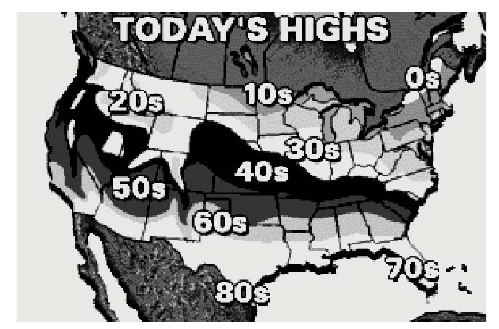
\includegraphics[width=0.5\textwidth]{./Exp1/pic/image1.png}
    \end{center}
    \caption{Temperature of Different Places in the United States}
    \label{fig:temp_field}
\end{figure}

The electric field (as well as the magnetic field) is a vector field, because a vector (rather than a scalar) is associated with each position. The direction and magnitude of an electric field at any point in space tells you the direction and magnitude of electric force that a  unit test charge would experience at this position. \myskip

A line that is formed by connecting electric field vectors and follows the direction of the field is called a \underline{field line}. A field is considered uniform if the field lines are parallel. The potential associated with such a field increases linearly with the distance traveled along the field lines.

\subsection{Equipotential Contours for Gravity}

A topographical map is a map with lines that indicate contours of the same height. On such a map, a mountain may look like figure \ref{fig:topograph}

\begin{figure}[h]
    \begin{center}
        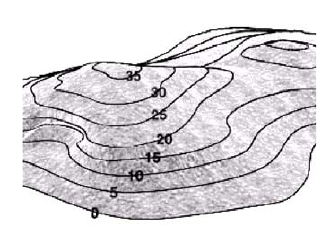
\includegraphics[width=0.4\textwidth]{./Exp1/pic/image2.png}
    \end{center}
    \caption{A Topographical Map}
    \label{fig:topograph}
\end{figure}

These contours of the same height $(h)$ are equi-height lines or, if you think in terms of potential energy $(U = mgh)$, they are equipotential lines. That is, every point on the contour has the same value of potential energy. So as you move along a contour, you do not change height, and therefore you neither gain nor lose potential energy. Only as you step up or down the hill do you change the energy. \myskip

There are a few general properties of equipotential contours:
\begin{itemize}
    \item They never intersect. (A single point cannot be at two different heights at the same time, and
therefore it cannot be on two different contours.)
    \item They close on themselves. (A line corresponding to constant height cannot just end.)
    \item They are smooth curves, as long as the topography has no sharp discontinuities (like a cliff).
\end{itemize}

\subsection{Analogy between Electric and Gravitational Potentials}

Electric potential is analogous to gravitational potential energy. Of course, gravitational potential energy arises from any object (with mass), whereas the electric potential arises only from charged objects. \myskip

As in mechanics, the absolute value of potential is not important. The differences in potential are the quantities that have physical meaning. In a real problem, it is usually best to choose a reference point, define it as having zero potential, and refer to potentials at all other points relative to the that point. Similarly, topographic height is usually reported relative to the reference at sea level.

\subsection{Field Lines}

Let's exploit our analogy of mountains and valleys a bit further for electric fields. Electric field lines indicate the electric force on a test charge (magnitude and direction). Gravitational field lines tell us about the gravitational force on a test mass (magnitude and direction) -- the direction it tends to roll down the hill and the acceleration it experiences during its journey. So if we carefully track a marble as we roll it down the hill in small increments, we can obtain a ``field-line''.  \myskip

What is the characteristic of a field line? Think about placing a marble on an inclined hillside.  Which way will it roll if you release it? It will always roll in the direction of steepest descent, and this direction is always perpendicular to the contours that indicate equal height (which we have been referring to as equipotential lines). \myskip

So it is for the electric case: if we know the equipotential lines, we can draw the field lines such that each one is perpendicular to each equipotential line. Figure \ref{fig:equi_field} and \ref{fig:field_dipole} both show equipotential lines (dashed lines) and the corresponding field lines (solid lines).

\begin{figure}[h]
    \begin{center}
        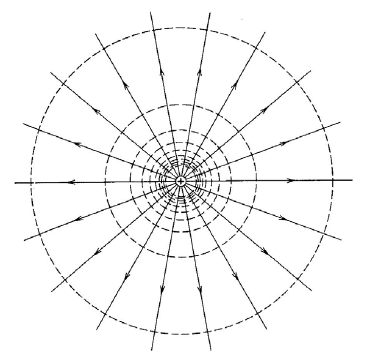
\includegraphics[width=0.5\textwidth]{./Exp1/pic/image3.png}
    \end{center}
    \caption{Equipotential Lines and Field Lines of a Single Charge}
    \label{fig:equi_field}
\end{figure}

Keep in mind that when equipotential lines are closer together, the potential is changing faster! This means we have steeper changes in height for gravitational field lines for example.

\begin{figure}[h]
    \begin{center}
        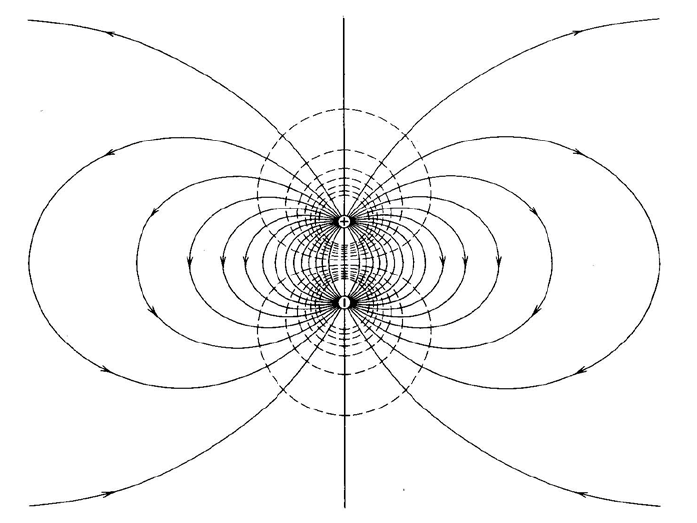
\includegraphics[width=0.6\textwidth]{./Exp1/pic/image4.png}
    \end{center}
    \caption{Equipotential Lines and Field Lines of a Pair of Opposite Charges}
    \label{fig:field_dipole}
\end{figure}

There are also a few rules for field lines:
\begin{itemize}
    \item Field lines always begin and end on charges. (They often terminate on material surfaces, but that is because there are charges on those surfaces.)
    \item They never intersect each other (except at electric charges, where they also terminate).
    \item They always intersect equipotential lines perpendicularly!
    \item They are usually smoothly continuous (except if they terminate).
\end{itemize}

\subsection{Metal Surfaces}

It turns out that for electrical phenomena, metals are equipotentials. So, by using metals, we can impose some unusually shaped equipotential lines and determine the corresponding field lines. \myskip

Metals are always equipotentials because:
\begin{enumerate}
    \item they are excellent conductors of electric charge, and
    \item they have an abundant supply of freely moving negative charges (electrons).
\end{enumerate}

Based on these two properties, we can understand that, if a field line were to penetrate a metal surface, these electrons would feel electric forces to move them through the material in the direction opposite to that of the electric field (since they are negative) until they would be forced to stop upon encountering the metal surface on the other side. Therefore, the free electrons ultimately distribute themselves along the surface of the metal so that there is a net negative charge on one side of the conductor and a net positive charge on the other (from where the electrons have fled). This realignment of the free electrons creates a field that precisely cancels the imposed field resulting in no net field, and the \underline{remaining} free charges inside the conductor then feel no force and don't move! Hence, field lines imposed from outside always end on metal surfaces (which they intersect perpendicularly), and the surface (with the entire interior) is an equipotential.

\subsection{Electric Shielding Theorem}

As just discussed, whenever a piece of metal is placed in an electric field, the entire metal will remain an equipotential. That is, every point in the metal will be at the same potential as every other point. No field lines penetrate through metals. \myskip

What happens if we take an enclosed container of metal of arbitrary shape, say a tin can, and put it into an electric field? Since no field gets through the metal, there must be no electric field inside the can. This means that every point inside the container, as well as all points on the container surface must be at the same potential. (If they were not, then there would be differences in the potential and therefore an electric field.) \myskip

Let’s return to our analogy of gravity equipotentials in hills and valleys, with field lines in the direction a marble would roll down the hill. Consider how a frozen lake would look on such a contour map. The surface of the lake has the same gravitational potential energy at all points, therefore if you place a marble on the frozen surface of the lake, the marble will not roll anywhere. In other words, there is no component of the gravitational field along the surface of the lake to push the marble. Similarly, there is no electric field on the inside of a closed metal container to push the charges around, and the entire interior is therefore a constant equipotential surface.

\subsection{Remarks for Experts}

\begin{enumerate}
    \item  The gravitational analogy operates in only two dimensions: the horizontal coordinates describing the surface of the lake. When discussing electrical fields we should, in principle, take into account all three dimensions. The analogy of the lake surface for the electrical case is the entire volume (three dimensions) of the interior of the can. For this experiment, we ``cheat'' a little by looking at electric field within a two dimensional world of slightly conducting paper. But the field and potential arrangements are as one expects for electrostatic phenomena in a two dimensional system.
    \item To shield electric field, we actually don't need a metallic surface that is completely closed; a closed cage of wire mesh (Faraday cage) is sufficient. So a sedan will work like a Faraday cage, but a convertible will not since it is not closed at the top.
\end{enumerate}

\section{Experiments}

In this experiment, we use pieces of slightly conductive paper, electrodes, and metallic paint to determine different equipotential and field configurations. Before we actually start our measurements we will have to draw the shapes on the conductive paper using the metal paint. The metal paint will take a few minutes to dry.

\subsection{Preparation of the Conductive Paper}

Take four pieces of conductive paper -- three full-sized and one thin strip and paint on them with the metallic paint according to the following instructions. Each shape drawn by the metal paint is an equipotential curve. By connecting the pins to areas covered with paint, we can determine the field configurations between different equipotential shapes.\myskip

\begin{minipage}[h]{0.55\textwidth}
    \begin{enumerate}
        \item Leave the first piece of paper blank.
        \item On the second piece of paper paint two parallel plates. Use a piece of cardboard provided to get sharp edges with the paint. Don't use the rulers!
        \item On the third piece of paper paint a closed loop of any shape that does not enclose an electrode.
        \item Take the thin strip and paint a line on each short end of the strip.
    \end{enumerate}
\end{minipage}
\begin{minipage}[h]{0.45\textwidth}
    \begin{flushright}
        \vspace{0.5cm}
        \begin{tikzpicture}[scale=0.8]
            \draw (0,0) rectangle (-3,-2.5);
            \draw[line width=4pt] (-0.7,-0.5) -- (-0.7,-2);
            \draw[line width=4pt] (-2.3,-0.5) -- (-2.3,-2);
        \end{tikzpicture}
        \vspace{0.3cm}

        \begin{tikzpicture}[scale=0.8]
            \draw (0,0) rectangle (3,2.5);
            %\draw[line width=2pt] (0.7,1.25) to [bend left=70] (1.5,2.1) to[bend right=20] (2.3,1.25) to [bend left=30] (1.8,0.5) to [bend right=40] (1.2,1) to [bend right=70] (0.7,1.25);
            \draw[line width=2pt,rounded corners=3pt] (0.7,1.25) -- (1.5,2.1) -- (2.3,1.25) -- (1.8,0.5) -- (1.2,1) -- (0.4,0.6) -- cycle;
        \end{tikzpicture}
        \vspace{0.3cm}

        \begin{tikzpicture}[scale=0.8]
            \draw (0,0) rectangle (5,0.8);
            \draw[line width=4pt] (0,0) -- (0,0.8);
            \draw[line width=4pt] (5,0) -- (5,0.8);
        \end{tikzpicture}
    \end{flushright}
\end{minipage}

\myskip
\noindent Hints:
\begin{enumerate}
    \item You get the best results if you stay at least 1-2$\,\mathrm{cm}$ away from the edges of the paper. Also make sure that the pins are always in contact with the paper. (Otherwise the experiment does not work!) Be careful not to make the holes too big or the pins will no longer be in contact with the paper.
    \item Give the metal paint enough time to dry! First paint all the configurations you will use on the conductive paper. While they dry, get started on the two point-charge arrangement.
    \item Make sure you're not accidentally touching the paper when making measurements!
\end{enumerate}

\subsection{Setup of the Voltage Source}

\begin{itemize}
    \item ``OUTPUT A'' of the power supply will be used in this experiment to provide a constant potential difference of 10 volts.
    \item Turn the ``A VOLTAGE'', the ``A CURRENT'', the ``B VOLTAGE'', and the ``B CURRENT'' control knobs located on the right side of the front panel counterclockwise to the ``MIN'' position.
    \item Set the ``A/B OUTPUT'' switch located on the upper right of the front panel to the ``INDEPENDENT'' setting, and set the ``A/B METER'' switch located between the two meters on the front panel to the ``A'' setting.
    \item Turn the power on by using the button located on the left of the front panel.
    \item Slowly turn the ``A VOLTAGE'' output knob until the voltage reads 10 volts. After doing this, do not make any further changes on the power supply for the remainder of the experiment. (The current meter will stay at a zero reading.)
    \item Connect two cables to the ``A OUTPUT ($0\sim 20\,\mathrm{V}\  0.5\,\mathrm{A}$)'' of the power supply (red and black poles) and then connect these cables to two of the yellow-metallic pins.
\end{itemize}

NOTE: To use the digital multimeter as an appropriate voltmeter for this experiment: turn the multimeter power on, select ``DC'' (button in out position), select ``VOLTS'' (push button in), set range to ``2 VOLTS'', and connect your voltage-measuring cables to the ``$\mathrm{V}$--$\Omega$'' and the ``COM'' jacks.

\subsection{Equipotential and Field Lines}

\begin{itemize}
    \item Connect two cables to the output of the power supply (black and red poles) and two of the yellow-metallic pins as described in the last step of the previous part. These are your output pins.
    \item Take one additional cable and connect one end to the black pole of the multimeter and the other to a different metallic pin. This will be your reference pin. Take the pen-like pin and plug it into the red pole of the multimeter. This pin will be your measuring probe.
    \item Take an empty sheet and put the two output pins on it to act as point-like sources. Push the pins in only a little bit and not all the way through.
    \item Insert the reference pin at an arbitrary position and move the measuring probe until the multimeter shows a value of zero. This means that the two points are at the same potential. Mark this position with one of the red markers provided. Search for more equipotential points until you have enough to draw an equipotential contour connecting them.
    \item Move the reference pin to a new position and construct another equipotential line.
    \item Repeat for a total of about 5 equipotential lines.
    \item Given these equipotential lines, draw about 5 field lines using the yellow pen. Remember that the field lines and equipotential lines always intersect perpendicularly.
    \item Do your equipotential and field lines show the symmetries you would expect for this system? Just what symmetries does/should this system have?
    \item Obtain the equipotential and field lines for the parallel-plate configuration as well. (Stick the two pins from the function generator into the metal paint-covered part of the paper, after the paint has dried!).
    \item Are the equipotential lines as you expect them?
    \item What the major problems and uncertainties in this part?
\end{itemize}

\subsection{Electric Shielding Theorem}

Take the sheet with the conducting loop on it, and set up an electric field. You need the reference pin as in the previous part. Put it somewhere either within the loop or on the rim of it.\myskip

Put the reference pin anywhere within the closed surface or on its rim, and check that any point within the loop has the same potential as the reference pin. This demonstrates that all points within the closed loop have the same potential.
\begin{itemize}
    \item What do you conclude about the shielding theorem? Does it hold or not?
    \item What would happen with your readings if you had drawn the loop badly such that the loop was not perfectly closed?
\end{itemize}

\subsection{Linear Increase in Potential}

The purpose is to verify that the potential increases linearly with distance as you move the probe from one end to the other.\myskip

Take the small strip and connect the two output pins to the metal covered ends. This produces a potential difference between the ends. Take the reference pin and remove the pin from the end. (You only need the cable and not the pin.) Connect it to one of the output pins. Take the measuring probe and measure how the voltage increases along the center of the strip as you move further away from the reference point.\myskip

Plot a voltage vs.\ distance graph. And use LINEST to determine the best-fit line and intercepts.
\begin{itemize}
    \item Do the points fall on a reasonably straight line?
    \item How do you interpret the slope and intercept of this line?
    \item Is the field between the two poles uniform?
    \item What would you observe if you measured the voltage tpwards the outside of the strip rather than along the center?
\end{itemize}

\section{Applications}

\begin{figure}[h]
    \begin{center}
        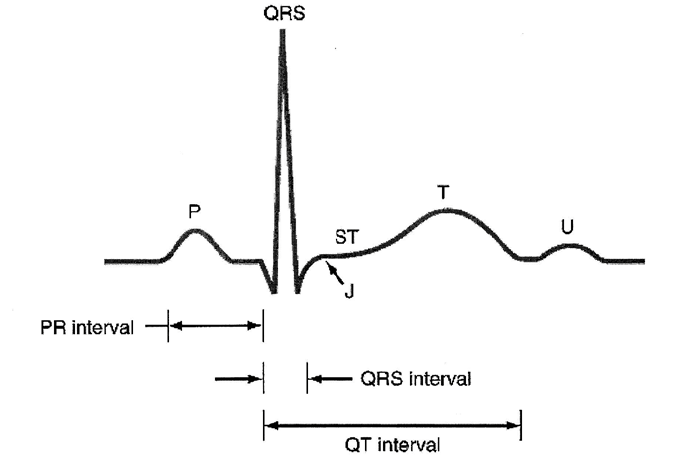
\includegraphics[width=0.6\textwidth]{./Exp1/pic/image5.png}
    \end{center}
    \caption{Sample Voltage Pattern for ECG}
    \label{fig:ecgpattern}
\end{figure}

The canonical example in medicine for measuring voltage potentials and displaying them (with an oscilloscope) are ECG (Electrocardiography) and EEG (Electroencaphelography). The basic idea of these two standard devices is fairly simple: by measuring the potential difference in time between two points (or usually several pairs of points) one gets a nice direct insight into the activity of the heart (brain) and can therefore detect dysfunctions easily. Let us, for example, take a closer look at how an ECG works: If you record the electrical potential between two points along your chest you can record the voltage pattern shown in figure \ref{fig:ecgpattern} (in time).\footnote{Remember: The ECG only shows the electrical polarization of the heart muscle. It does not show the contraction of the heart muscle!} \myskip

As you can see, the pattern observed can be split into different parts: At first the atrial cells are depolarized, giving the first signal (P wave). (This signal is relatively weak due to the small mass of the atrium.) After a delay one gets the QRS complex, which indicates the depolarization (wave) of the ventricles. After another delay one gets the T wave, which comes from the repolarization of the heart. \footnote{The interpretation of the U wave is still not yet 100\% understood} What do all these results, obtained from the heart as a total, mean in terms of processes going on in the single cells? The next figure \ref{fig:ventricule} shows the measurement by your ECG in comparison to the potential in a single cell in a ventricle (obtained using a different method). First we recall that the interior and the exterior of the cell in their standard state have different ion concentrations and are therefore at different electrical potentials. (That is the zero line in the graph.) In the depolarization phase the ion channels in the cell membrane open and a flow of $\mathrm{K}^+$ ions changes the potential inside the cell very rapidly. After this rapid change in potential one gets a plateau, which is mainly due to the inflow of $\mathrm{Ca}^{++}$ ions into the cell. (The $\mathrm{Ca}^{++}$ ions are much bigger than the $\mathrm{K}^+$ ions, because they have a much larger hydrogen cover surrounding them and they diffuse much slower through the ion channels.) Finally in the repolarization phase the ion channels close again and the ion pumps in the cell membrane reestablish the initial ion concentrations. \myskip

\begin{figure}[h]
    \begin{center}
        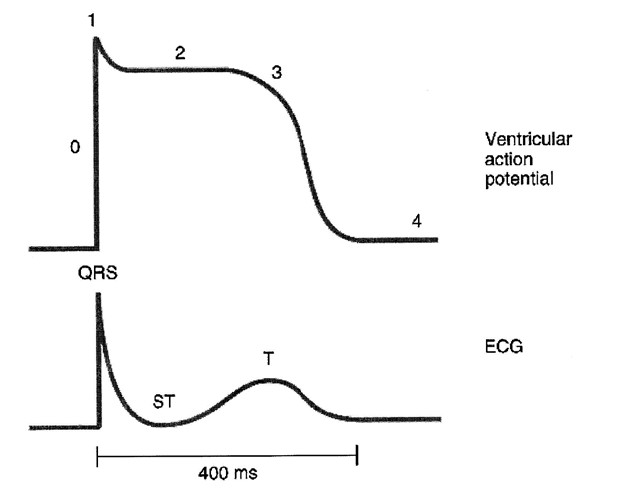
\includegraphics[width=0.55\textwidth]{./Exp1/pic/image6.png}
    \end{center}
    \caption{Comparison with Ventricular Potential}
    \label{fig:ventricule}
\end{figure}

How can you now take advantage of this method for a diagnosis? First of all you don't want to take the measurements only along one single axis or plane, since e.g.\ if an infarction occurs on the front or back wall of your heart you are probably going to miss it. These days the usual way to get a 3-D picture of the position of the heart axis\footnote{The heart axis is a simplified concept of the locations of the electrical potentials in the heart. One can think of the heart axis as a vector sympolizing the (physical) axis of the heart.} is obtained by measuring with multiple channels simultaneously between the points indicated in figure \ref{fig:channels}. (The contacts with an R are placed on the patients back.) \myskip

\begin{figure}[h]
    \begin{center}
        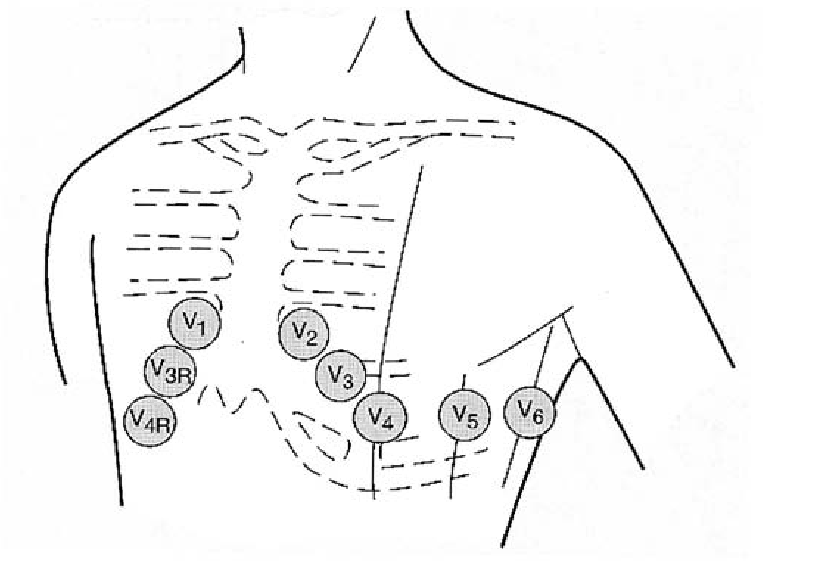
\includegraphics[width=0.5\textwidth]{./Exp1/pic/image7.png}
    \end{center}
    \caption{Channels of Measurement}
    \label{fig:channels}
\end{figure}

\begin{figure}[h]
    \begin{center}
        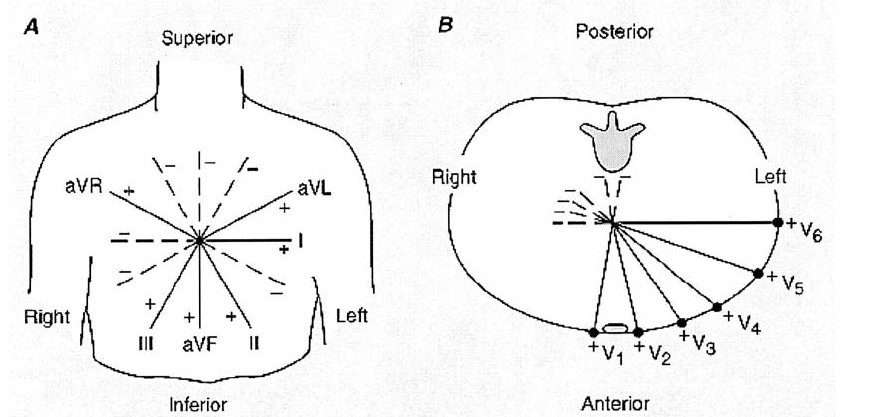
\includegraphics[width=0.8\textwidth]{./Exp1/pic/image8.png}
    \end{center}
    \caption{Electric Potentials and Information}
    \label{fig:heartcomp}
\end{figure}

From the location and amplitude of the main vector (axis) one can see for example if the muscle mass is increased on one side of the heart (hypertrophy). In that case the main vector is tilted.\footnote{Also in pregnant women the heart as a total is slightly repositioned and therefore the electrical axis is a little bit off.} Another thing to look for is if the depolarization and repolarization was performed properly. For example if the ion channels in a certain region of the heart are destroyed by an infarction, then the electric potential between the depolarization and repolarization phase does not reach the zero level. By looking at your data you can not only locate the infarction, but also read off additional information, e.g.\ if the infarction cilled the tissue through all of the heart wall or only parts of it. (That determines your treatment of the patient!) \myskip

You can see that you can get a lot of useful information if you look at electrical potentials (and their change in time), as shown in figure \ref{fig:heartcomp}. \myskip

Textbook references:
\begin{itemize}
    \item Stein: \emph{Internal Medicine}
    \item Harrison's \emph{Principles of Internal Medicine}
\end{itemize}

\newpage
\section{Lab Preparation Examples}

\noindent\underline{Field Lines}: Given the following equipotential lines, draw 5-10 field lines on each diagram. \myskip

\begin{minipage}[h]{0.95\textwidth}
    1.\begin{center}
        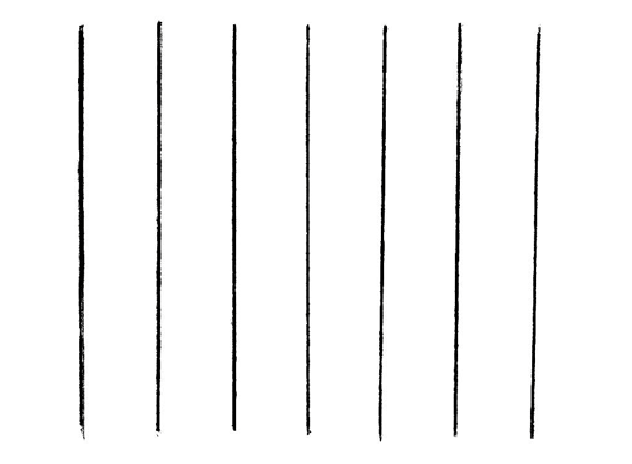
\includegraphics[width=0.7\textwidth]{./Exp1/pic/image9.png}
    \end{center}
\end{minipage}

\begin{minipage}[h]{0.95\textwidth}
    2.\begin{center}
        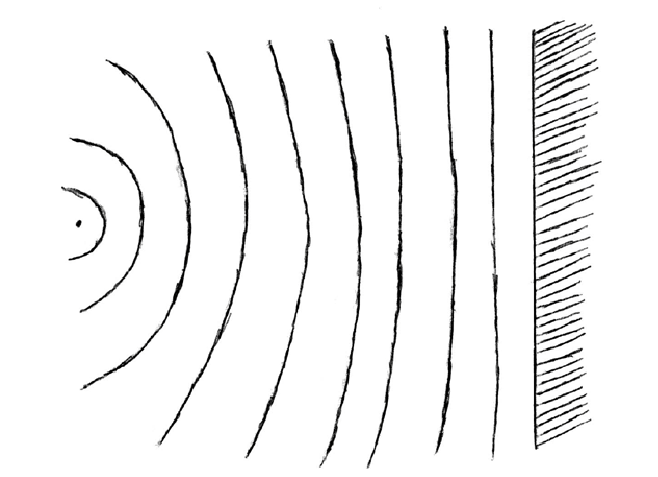
\includegraphics[width=0.7\textwidth]{./Exp1/pic/image10.png}
    \end{center}
\end{minipage}

\begin{minipage}[h]{0.95\textwidth}
    3.\begin{center}
        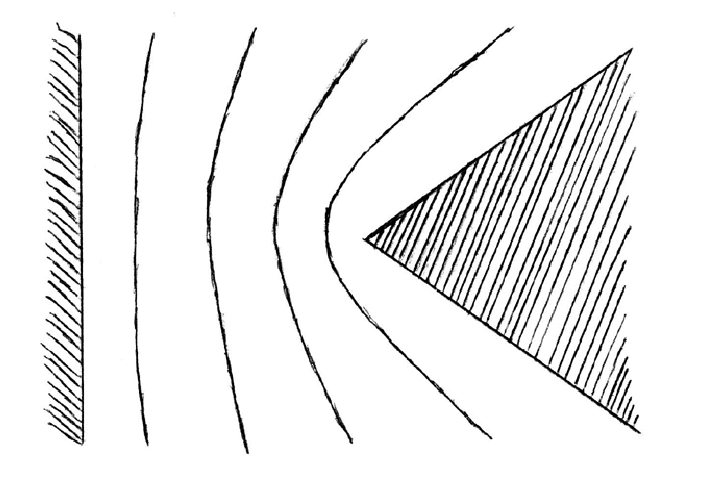
\includegraphics[width=0.7\textwidth]{./Exp1/pic/image11.png}
    \end{center}
\end{minipage}

\begin{minipage}[h]{0.95\textwidth}
    4.\begin{center}
        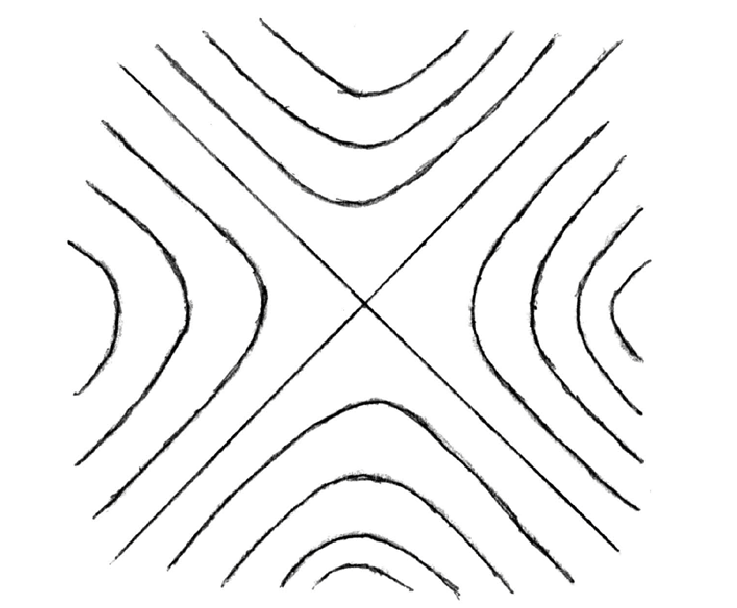
\includegraphics[width=0.7\textwidth]{./Exp1/pic/image12.png}
    \end{center}
\end{minipage}

\noindent\underline{Shield Theorem} \myskip

5. Explain in a few sentences why you might be safe inside your new Volkswagen Beetle even when struck by a bolt of lightning.

%\chapter{DC Circuits}
\begin{comment}
\section{Introduction}

In this experiment you are going to construct a slide-wire potentiometer and use it to measure the electromotive force (emf) of a battery. The emf is a somewhat misleading term, since it does not refer to a force at all, but to the voltage (or energy per unit charge) made available by the battery. \myskip

You may be wondering why we cannot simply attach a voltmeter (device that measures voltage) to the battery and say that the voltage we read is the emf of the battery. The reason for this is because the battery has its own internal resistance, and when the voltmeter sends current through the battery to measure the voltage, the internal resistance of the battery affects the voltage measured. Therefore, in order to accurately measure the emf of a battery, we have to use a device that does not draw any current through the battery. The potentiometer is one such device that will accomplish this goal. \myskip

The potentiometer is also used to measure the small voltage across a thermocouple, which is a device used to determine temperature differences by measuring the thermal emf produced at the junctions of dissimilar metals. In this case, the thermal emfs cannot supply sufficient current to be measurable on an ordinary meter, so a potentiometer is used.

\section{Theory}

\subsection{Resistance of a uniform wire}

Consider a uniform wire of length $l$ and cross-sectional area $A$ with a potential difference $\Delta V = V_b - V_a$ maintained across it, as shown in figure \ref{fig:reswire}

\begin{figure}[h]
    \begin{center}
        %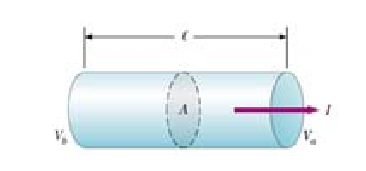
\includegraphics[width=0.25\textwidth]{./Exp2/pic/image1.png}
        \begin{tikzpicture}[scale=0.4,font=\footnotesize]
            \draw (-3.5,1.5) -- (3.5,1.5);
            \draw (-3.5,-1.51) -- (3.5,-1.51);
            \draw (3.5,0) ellipse (0.75 and 1.5);
            \begin{scope}
                \clip (-4.5,1.5) rectangle (-3.5,-1.5);
                \draw (-3.5,0) ellipse (0.75 and 1.5);
            \end{scope}
            \node at (0,0) {$A$};
            \draw[dashed] (0,0) ellipse (0.75 and 1.5);
            \draw[very thick,->] (2,0) -- (5,0) node[right] {$I$};
            \draw (-3.5, 1.6) -- (-3.5, 3);
            \draw (3.5, 1.6) -- (3.5, 3);
            \draw[->] (0.3, 2.6) -- (3.4,2.6);
            \draw[->] (-0.3, 2.6) -- (-3.4,2.6);
            \node at (0,2.6) {$l$};
            \node at (5,-1.5) {$V_a$};
            \node at (-5,-1.5) {$V_b$};
        \end{tikzpicture}
    \end{center}
    \caption{Resistance of a Uniform Wire}
    \label{fig:reswire}
\end{figure}

The current $I$ that this potential difference produces can be obtained once we know the resistance $R$ of this wire:
\begin{equation}
    I = \frac{\Delta V}{R}
\end{equation}
The resistance of the wire is proportional to its length (the longer the wire, the ``harder'' it is for electrons to travel from $b$ to $a$) and inversely proportional to its cross-sectional area (the wider the wire, the ``easier'' it is for electrons to travel from $b$ to $a$):
\begin{equation}
    R = \rho\frac{l}{A}
\end{equation}
where the constant of proportionality $\rho$ is called the resistivity and is a characteristic of the material the wire is made of. \myskip

In our experiment, by moving the slider $P$, we effectively change the length of the wire $MP$, while of course the area $A$ and resistivity $\rho$ remain the same. That is why the resistance between $M$ and $P$ is proportional to the length $MP$.

\subsection{Kirchoff's Rules}

Simple circuits can be analyzed using the expression $V = IR$ and the rules for series and parallel combinations of resistors. Very often, however, it is not possible to reduce a circuit to a single loop. The procedure for analyzing more complex circuits is greatly simplified if we use two principles called Kirchhoff's rules.

\begin{enumerate}
    \item Junction Rule: The sum of the currents entering any junction in a circuit must equal the sum of the currents leaving that junction:
        \begin{equation}
            \sum I_\text{in} = \sum I_\text{out}
        \end{equation}
        This is basically just the statement of conservation of electric charge. For example if we have a junction as shown in figure \ref{fig:junction}, then we have $I_1 = I_2 + I_3$.
        \begin{figure}[h]
            \begin{center}
                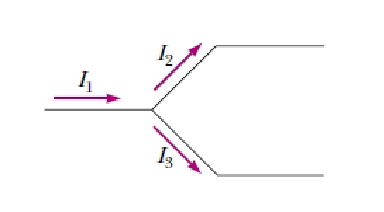
\includegraphics[width=0.3\textwidth]{./Exp2/pic/image2.png}
            \end{center}
            \caption{A Sample Junction}
            \label{fig:junction}
        \end{figure}
    \item Loop Rule: The sum of the potential differences across all elements around any closed circuit loop must be zero:
        \begin{equation}
            \sum_\text{closed loop} V = 0
        \end{equation}
        This rule simply follows from the conservation of energy.
\end{enumerate}

When applying Kirchhoff's second rule in practice, we imagine traveling around some loop and consider changes in electric potential, bearing in mind the following sign conventions:

\begin{figure}[h]
    \begin{center}
        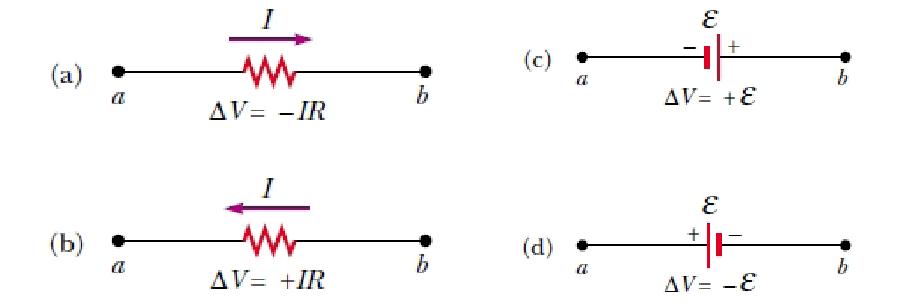
\includegraphics[width=0.6\textwidth]{./Exp2/pic/image3.png}
    \end{center}
    \caption{Sign conventions for Kirchhoff's Second Rule}
    \label{fig:kirchhoff2}
\end{figure}
\begin{itemize}
    \item If a resistor is traversed in the direction of the current, the potential difference across the resistor is negative (figure (a)).
    \item If a resistor is traversed in the direction opposite the current, the potential difference will then be negative (figure (b)).
    \item If a source of emf (assumed to have zero internal resistance) is traversed in the direction of the emf (from $-$ to $+$), the potential difference will be positive (figure (c)).
    \item If it is traversed in the direction opposite the emf (from $+$ to $-$), the potential difference will be negative (figure (d)).
\end{itemize}

In practice, for a given circuit diagram, we first label all the known and unknown quantities and assign a direction to the current in each branch of the circuit. Although the assignment of current directions is arbitrary, you must adhere rigorously to the assigned directions when applying Kirchhoff's rules. After applying Kirchhoff's rules to junctions and loops as necessary, we simply need to solve the resulting equations simultaneously for the unknown quantities. If some current turns out to be negative, that simply means that its direction is opposite to that which we assigned, but its magnitude will be correct.  

\newpage
\section{Experiment}

\subsection{Setup}

A schematic diagram of the potentiometer is shown in figure \ref{fig:potcircuit}, where:

\begin{figure}[h]
    \begin{center}
        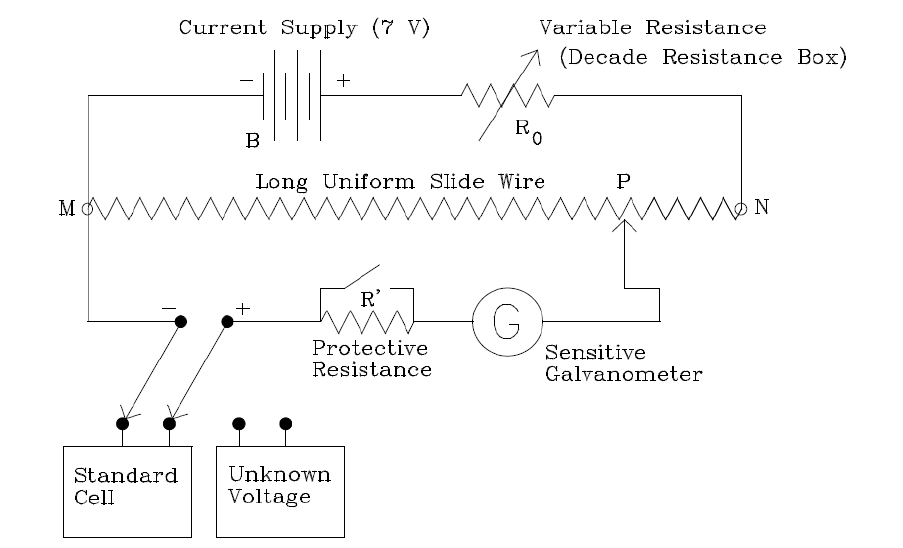
\includegraphics[width=0.8\textwidth]{./Exp2/pic/image4.png}
    \end{center}
    \caption{Circuit Diagram of the Potentiometer}
    \label{fig:potcircuit}
\end{figure}

\begin{itemize}
    \item $B$ is a stable current source with a constant voltage greater than any voltage to be measured.
    \item $MN$ is a long wire of uniform cross-section.
    \item $P$ is a sliding contact which varies the length of wire, and therefore the resistance between $M$ and $P$.
    \item $R_0$ is a decade resistance box, which is a resistor whose resistance can be varied within a certain range by turning knobs on the box. The resistance can be adjusted to reduce the total voltage across $MN$.
    \item $G$ is a sensitive galvanometer which indicates zero current when the needle deflects neither to the left nor to the right. A galvanometer is a type of ammeter (device for measuring current) that is used for direct current circuits.
    \item $R'$ is a protective resistance to limit the current through the galvanometer when the potentiometer is not balanced. The shorting button bypasses $R'$, to increase the sensitivity in determining a null current, and should be used only after an approximate balance is obtained.
\end{itemize}

\subsection{Standard Cell Calibration}\label{sec:standardcell}

Before each measurement, first adjust $R_0$, (the decade resistance box), so that the voltage across $MN$ is larger than the value of $V_x$ to be measured. Then use the standard cell to calibrate the potentiometer for this setting as described in the following paragraph.\medskip

In order to calibrate, the standard cell is connected to the circuit, and the movable contact $P$ is adjusted to a position $P_S$ at which the galvanometer reads zero. First do this with the shorting button open, and then, for a more precise reading, depress the shorting button and adjust the position of $P$ so that the galvanometer reads zero again. At this setting, the difference in potential between $M$ and $P$ is equal to the known value of $V_S$.

\subsection{Unknown Voltage}\label{sec:unknownvolt}

Next, the standard cell is replaced by a source of unknown voltage $V_x$, and the procedure is repeated to find a point $P_x$ where the galvanometer reads zero. The value of $V_x$ can then be determined from the ratio of the two distances along the slide wire ($MP_x$ and $MP_s$) along with the known value of $V_S$.\medskip

Perform this measurement for two sources of unknown voltage, first singly and then for the two cells in series. Make sure to follow the instructions in section \ref{sec:standardcell} before each measurement.\medskip

\textbf{CAUTION}: Never use a standard cell to supply current to a circuit; it is to be used only as a reference voltage when negligible current is drawn. Since drawing a large current would damage the cell, a large protective resistor has been built into the cell holder.

\subsection{Internal Resistance of a Battery}

As mentioned in the introduction, a battery can be considered as the equivalent of a source of chemical emf $\varepsilon$ in series with an internal resistance $r$. When a current $I$ is drawn from the cell, the voltage across the terminals of the cell will be $\varepsilon - Ir$. The maximum current that can be drawn from such a cell is thus $\varepsilon/r$. As a battery is used up, the value of $\varepsilon$ remains relatively constant, but the value of $r$ rises appreciably. \myskip

One way to determine $r$ would be to connect the cell to an external load, such as a light bulb, and measure both the voltage $V$ across the terminals of the cell and the current $I$ which is delivering to the load. Then the difference between $\varepsilon$, (measured in section \ref{sec:unknownvolt}), and $V$ would be $Ir$. \myskip

\begin{figure}[h]
    \begin{center}
        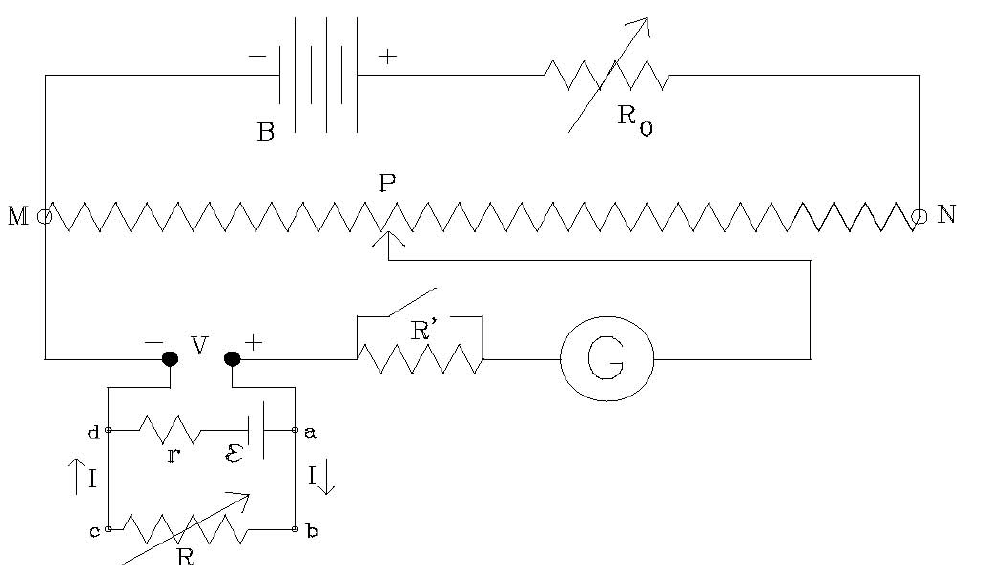
\includegraphics[width=0.8\textwidth]{./Exp2/pic/image5.png}
    \end{center}
    \caption{Circuit for Measuring Internal Resistance}
    \label{fig:internalres}
\end{figure}

However, you can alternatively determine $r$ without measuring $I$. To do this, connect a calibrated variable resistance $R$ (another decade box), as the load across the terminals to the battery, as shown in figure \ref{fig:internalres}. When $R$ is adjusted so that $V$ equals exactly half of the emf of the cell, $\varepsilon/2$, then the value of $R$ is just equal to $r$. This is so because, with the potentiometer balanced, the only current which flows in the external circuit is the current $I$ around the loop $abcd$. Thus we have the following equations:
\begin{equation}
    \varepsilon = IR + Ir,\qquad V = IR = \frac{\varepsilon}{2}
\end{equation}
Combining the above two equations we obtain:
\begin{equation}
    2IR = IR + Ir
\end{equation}
which can be simplified to yield:
\begin{equation}
    R = r
\end{equation}

To utilize this method, the best procedure is first to set $MP$ to half of the value it had for the measurement of $\varepsilon$ before $R$ was connected, that is, set the potentiometer to measure $\varepsilon /2$. Then adjust $R$ until the potentiometer is balanced at this setting.
\end{comment}



\chapter{Capacitance}

\section{Introduction}

In this lab, we will explore th behavior of capacitors in circuits and how they interact with other circuit elements. Specifically, we will examin the behavior of current and voltage for charging and discharging  circuits, which comprise a resistor and a capacitor in series.

\section{Theory}

A capacitor is a device for storing electric charge and energy. For simplicity, an ideal capacitor can be considered as a pair of parallel conducting metal plates, as shown in Figure \ref{fig:capacitor}. When a charge $+Q$ is placed on the upper plate and $-Q$ on the lower plate, a potential difference $V$ is established between the plates, and the quantities $Q$ and $V$ are related by the expression:
\begin{equation}
    Q = CV
\end{equation}
where the capacitance $C$ is determined by the size and separation of the plates.

\begin{figure}[h]
    \begin{center}
        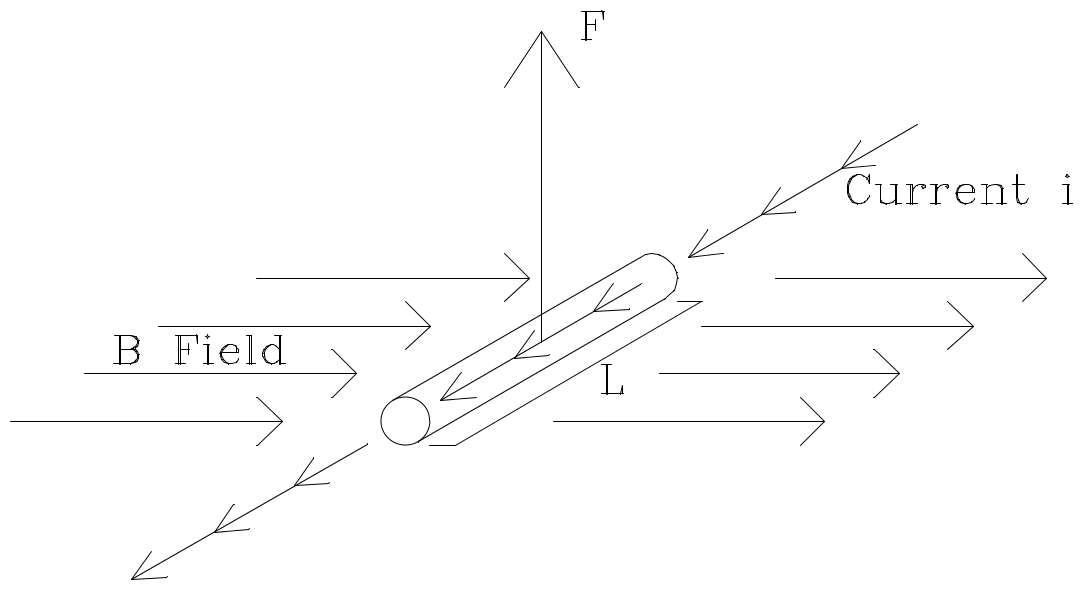
\includegraphics[width=0.5\textwidth]{./Exp4/pic/image1.png}
    \end{center}
    \caption{An Ideal Capacitor}
    \label{fig:capacitor}
\end{figure}

\subsection{Discharging a Capacitor}

If a wire is attached to the upper plate and then touched to the lower plate, charge will flow through the wire until the charge $q$ and potential difference $V$ are zero. (We will use $Q$ to indicate the initial charge and $q$ for the time dependent charge.) This process, known as discharging the capacitor, does not occur instantaneously. Instead, as the charge flows from one plate to the other, the potential difference decreases, and the current (or rate of change of charge) gradually diminishes. Since the rate of change is proportional to the amount of charge remaining, the current is initially large and then \emph{decays exponentially} with increasing time. Exponential growth or decay occurs whenever the rate of change of a quantity is proportional to the quantity present at that time. Exponentials are also characteristic of the growth rate of cells or organisms and the decay of radioactive isotopes.

The changing current which discharges a capacitor can be calculated as a function of time by considering the circuit shown in Figure  \ref{fig:capcircuit1}. The capacitor $C$ is initially charged by a battery of emf $\varepsilon$, placing a charge $Q = C\varepsilon$ on the plates. When the switch is closed, a current $I$ flows in the circuit, and according to Ohm's Law the voltage drop across the resistance is $IR$.

\begin{figure}[h]
    \begin{center}
        \includegraphics[width=0.4\textwidth]{./Exp4/pic/image2.png}
    \end{center}
    \caption{Discharging Circuit of a Capacitor}
    \label{fig:capcircuit1}
\end{figure}

The resistance may be a separate circuit element or merely the resistance of the wire itself. Since the sum of the voltage drops around the circuit must be zero, we obtain the equation:
\begin{equation}
    IR + \frac{Q}{C} = 0
\end{equation}

The equation can be rewritten in terms of charge alone from the definition of current, $\displaystyle I = dQ/dt \ \left(=\lim_{\Delta t\to 0} \frac{\Delta Q}{\Delta t}\right)$,
\begin{equation}
    R\frac{dQ}{dt} + \frac{Q}{C} = 0
    \label{eqn:diffcharge}
\end{equation}

Equation (\ref{eqn:diffcharge}) is a differential equation for $Q$ and has a solution which gives the time dependence of the charge
\begin{equation}
    Q(t) = C\varepsilon e^{-t/RC}
    \label{eqn:solcharge}
\end{equation}

Students familiar with calculus can verify this result by differentiating equation (\ref{eqn:solcharge}) and plugging back into equation (\ref{eqn:diffcharge}) to show that everything is satisfied. From the definition of current, $I = dQ/dt$, we find that
\begin{equation}
    I(t) = -\frac{\varepsilon}{R}e^{-t/RC}
    \label{eqn:dischargecurrent}
\end{equation}
Note that at $t=0$, when the switch is just closed, $I = -\varepsilon/R$. As time increases, the current $I(t)$ gets smaller and reaches zero as time goes to infinity.

\subsection{Charging a Capacitor}

The process of charging an uncharged capacitor has many similarities with the process of discharging discribed above. In this case, a battery with an emf of $\varepsilon$ volts is connected in series with a resistance $R$ and the capacitance $C$, as indicated in figure \ref{fig:chargecircuit}.

\begin{figure}[h]
    \begin{center}
        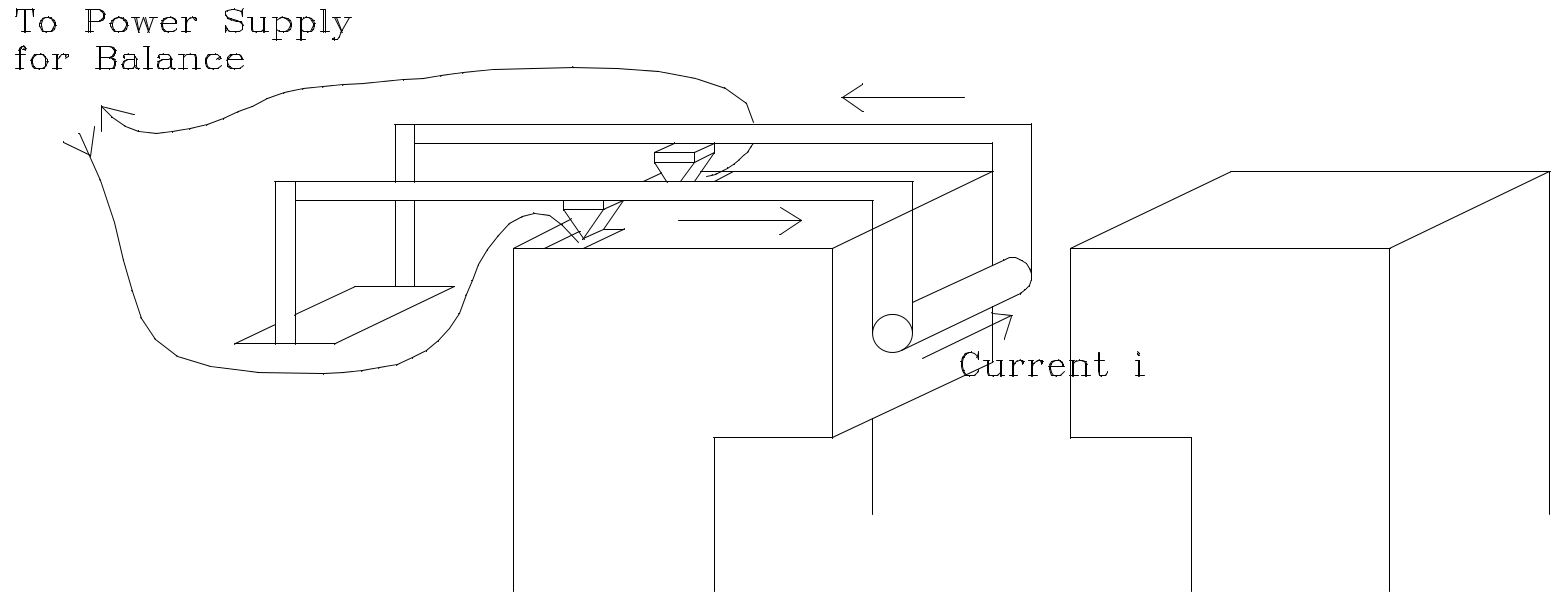
\includegraphics[width=0.4\textwidth]{./Exp4/pic/image3.png}
    \end{center}
    \caption{Charging Circuit of a Capacitor}
    \label{fig:chargecircuit}
\end{figure}

When the switch is first closed, there is no charge on the capacitor and thus no voltage across it, and the full voltage $\varepsilon$ appears across $R$, causing maximum current $I$ to flow. As the capacitor becomes charged, the voltage-drop $IR$ (and thus the current $I$) gradually decreases. $I$ approaches zero as the capacitor is charged toward its maximum potential difference of $\varepsilon = Q/C$. \myskip

The equation which indicates the sum of voltage drops around the circuit loop at any time during the charging is:
\begin{equation}
    \varepsilon = IR + \frac{Q}{C}
\end{equation}
Again, this can be converted to a \emph{differential equation}, the solution of which is:
\begin{equation}
    I(t) = \frac{\varepsilon}{R}e^{-t/RC}
    \label{eqn:chargecurrent}
\end{equation}

Comparing equation (\ref{eqn:dischargecurrent}) with (\ref{eqn:chargecurrent}), we note that the current for discharging a capacitor from a given potential $\varepsilon$ decreases in time identically to the current for charging the capacitor through the same resistance to the same final voltage $\varepsilon$. The difference in the sign of $I$ indicates, of course, that the two currents flow in opposite directions.

\subsection{Graphical Presentation of Exponential Decay}

In equations (\ref{eqn:dischargecurrent}) and (\ref{eqn:chargecurrent}), the symbol $e$ stands for the constant $2.71828\cdots$, the \emph{base of natural logarithms}. A graph of the function $y = ae^{-x/b}$ is given in figure \ref{fig:expgraph}, where $y=a$ at $x=0$ and then decays exponentially as $x$ increases, reaching a value of $y = ae^{-1} = 0.37a$ at $x=b$.

\begin{figure}[h]
    \begin{center}
        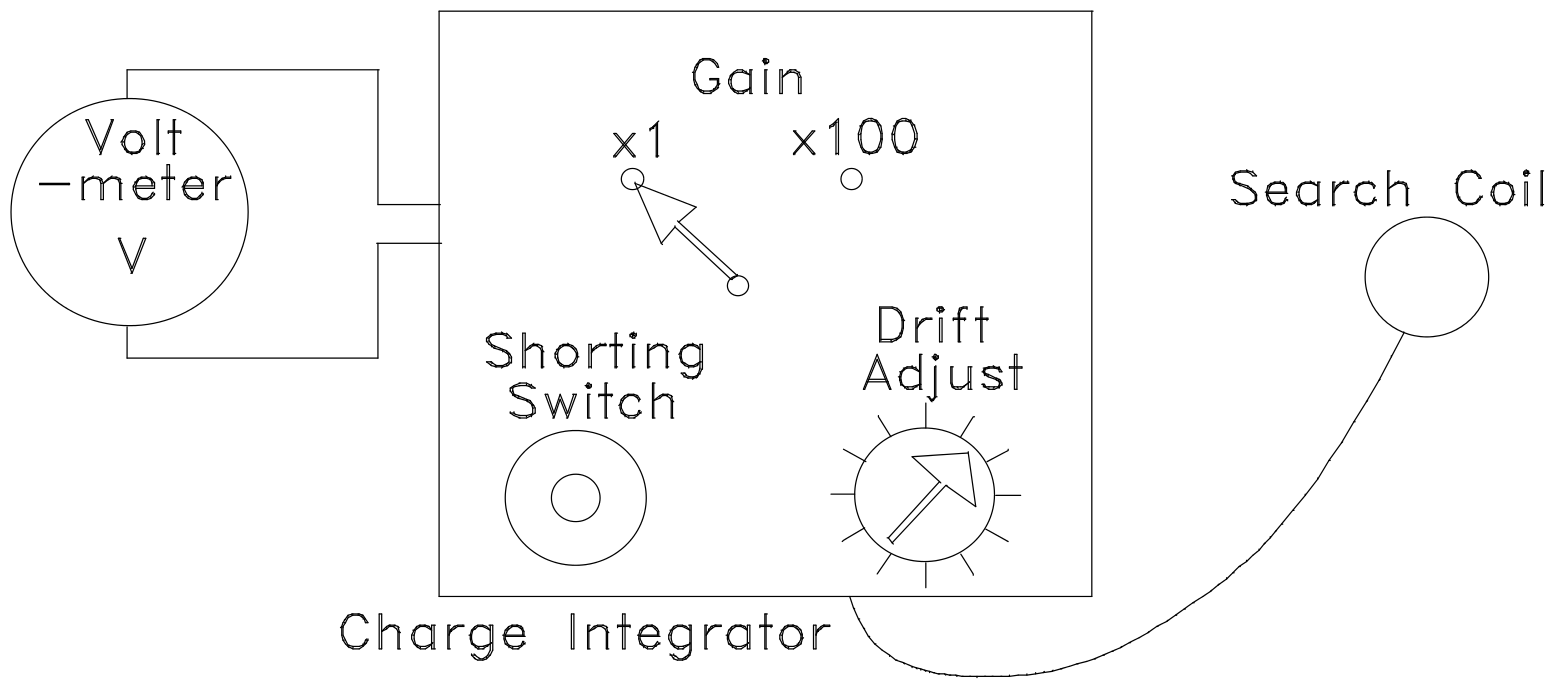
\includegraphics[width=0.9\textwidth]{./Exp4/pic/image4.png}
    \end{center}
    \caption{Graph of $y=ae^{-x/b}$}
    \label{fig:expgraph}
\end{figure}

Although it is possible to determine the values of $a$ and $b$ from experimental results plotted on such a curve, it is more informative to plot $\ln\,y$ versus $x$. Taking the natural logarithm (\ln) of $y=ae^{-x/b}$ yields:
\begin{equation}
    \ln\,y = \ln\,a + \ln\,e^{-x/b} = \ln\,a - \frac{x}{b}
    \label{eqn:logslope}
\end{equation}
which is a linear equation in $x$ representing a straight line with slope $-1/b$, if $\ln\,y$ is plotted against $x$ as in figure \ref{fig:logplot}. Linear equations are much easier to deal with. \myskip

\begin{figure}[h]
    \begin{center}
        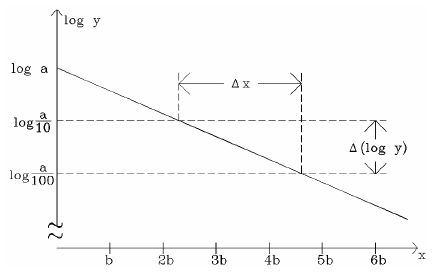
\includegraphics[width=0.8\textwidth]{./Exp4/pic/image5.png}
    \end{center}
    \caption{Plot of $\log\,y$ versus $x$}
    \label{fig:logplot}
\end{figure}

In the present experiment, $y$ repensents the current $I$; $x$ is the time $t$; $a$ is the initial value of $I$; and $b$ is the time constant $RC$. \myskip

\section{Procedure}

\subsection{Large RC-charging}

Figure \ref{fig:largerccharge} shows the circuit to be wired for measuring the current $I$ as a function of time for charging a capacitor $C$ through a resistance $R$ to a voltage $\varepsilon$. For this part of the lab you will use the bank of three large capacitors which are attached to a piece of wood with three switches and the label ``$30\,\mathrm{MFd}$''. (In this case the prefix ``M'' in MFd indicates micro, $\mu$, or $10^{-6}$.) Be sure to use a low-voltage (15 volts max.) power supply and to connect the positive terminal on the power supply to the positive terminal on the microammeter. Before closing the switch to the power supply and starting each new measurement, momentarily connect a low resistance across the capacitor in order to start with no charge on the capacitor plates. It is important to note that the resistance $R$ being used for your measurements is the internal resistance of the ammeter\myskip
\begin{figure}[h]
    \begin{center}
        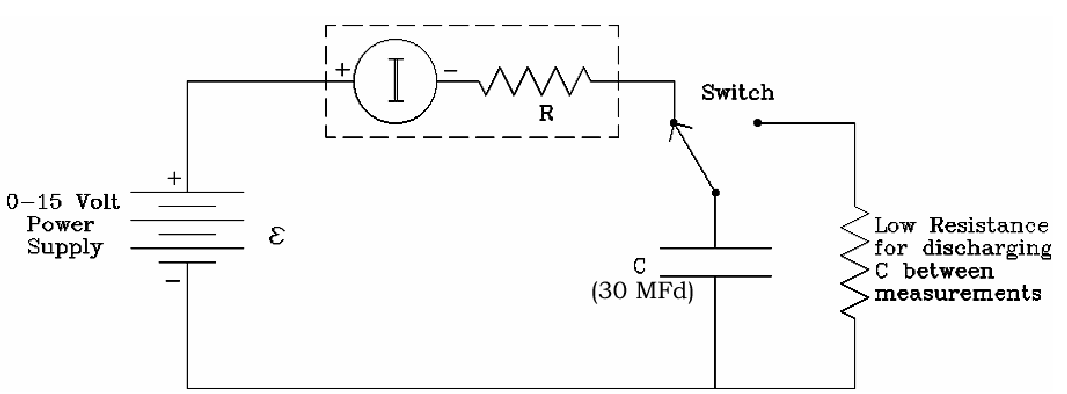
\includegraphics[width=0.8\textwidth]{./Exp4/pic/image6.png}
    \end{center}
    \caption{Large RC-charging Circuit}
    \label{fig:largerccharge}
\end{figure}

\begin{itemize}
  \item Measure $I$ at a series of time intervals after closing the switch. Plot $\ln,I$ vs. $t$ and construct a best-fit line.
  \item Use LINEST to determine the slope of your best-fit line with error.
  \item From your slope, determine the time constant $RC$ with error.
  \item Does your calculated time constant agree with the theoretical value $RC$ determined from the resistance and capacitance of the circuit?
\end{itemize}

\subsection{Large RC-discharging}

Use the circuit shown in Figure \ref{fig:largercdischarge} to measure the discharge current through the resistance $R$ of the same capacitors $C$ used in Part 1. You will use the same equipment as you used in Part 1 of the lab. \myskip

\begin{figure}[h]
    \begin{center}
        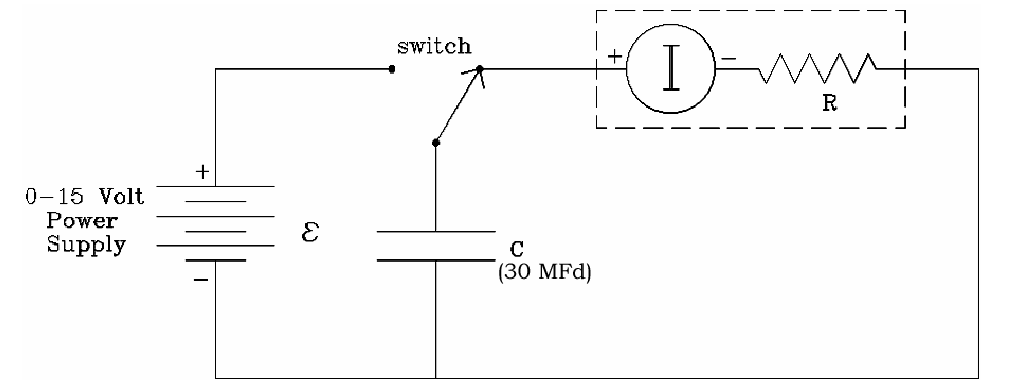
\includegraphics[width=0.65\textwidth]{./Exp4/pic/image7.png}
    \end{center}
    \caption{Large RC-discharging Circuit}
    \label{fig:largercdischarge}
\end{figure}

Before closing the switch to begin the measurement, momentarily connect the power supply directly across the capacitor in order to give it an initial charge.
\begin{itemize}
  \item Disconnect the power supply, close the switch, and measure $I$ as a function of time. Plot $\ln,I$ vs $t$ and construct a best fit line.
  \item Use LINEST to determine the slope of your best-fit line with error.
  \item From your slope, determine the time constant $RC$ with error.
  \item Does your calculated time constant agree with the theoretical value $RC$ determined from the resistance and capacitance of the circuit?
\end{itemize}

\subsection{A Relaxation Oscillator}

A neon bulb has the property of having a very high resistance (almost infinite) until the voltage applied to it is high enough to ``break down'' the gas, at which point the bulb lights and its resistance becomes very low. In this part of the lab you will use a high voltage power supply. Thus, \emph{it is essential that you are sure to use the small capacitor with a value of $0.082\,\mathrm{\mu F}$} rather than the bank of capacitors you use in the first two parts of the lab. Wire a neon bulb in parallel with the capacitor in the circuit of figure \ref{fig:relaxcirc}.\myskip

\begin{figure}[h]
    \begin{center}
        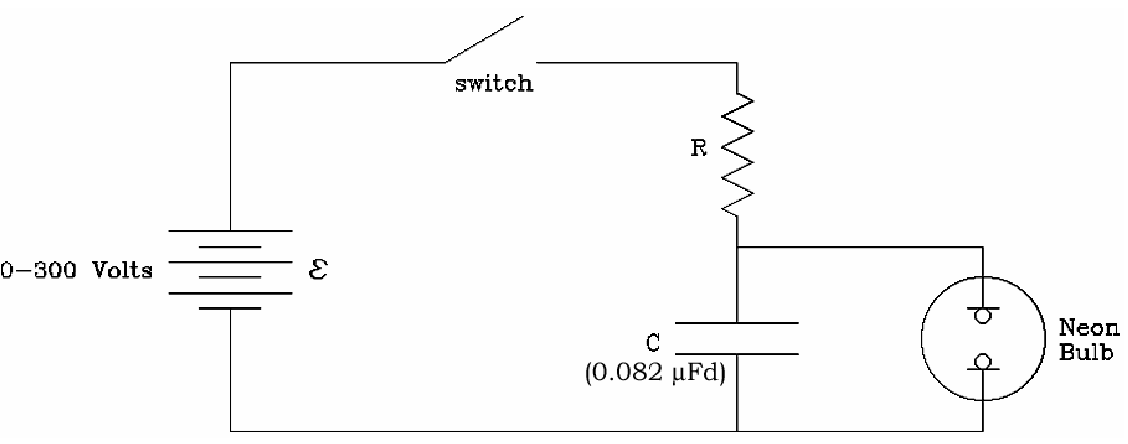
\includegraphics[width=0.75\textwidth]{./Exp4/pic/image8.png}
    \end{center}
    \caption{Relaxation Oscillator Circuit}
    \label{fig:relaxcirc}
\end{figure}

\textbf{CAUTION}: Since a relatively \underline{high-voltage} power supply is necessary for this part of the experiment, it is important not to touch any exposed metal parts of the circuit while the power supply is connected to the circuit and turned on, whether or not the switch is closed. Since the capacitor stores charge, \emph{it may be charged even if the voltage supply has been removed}. Be sure to discharge the capacitor fully by simultaneously touching an insulated wire to each end of the capacitor before touching any of the metal parts of the circuit.\myskip

When the switch is closed, the capacitor will start to be charged as in Part 1 with the time constant $RC$. The high resistance  of the neon bulb will have negligible effect on the circuit since it is wired in parallel. However, when the capacitor is charged to sufficiently high voltage, the neon bulb will light. The capacitor will then be quickly discharged through the bulb. If $R$ is sufficiently large, there will not be sufficient current to keep the bulb lit after the capacitor is discharged. The bulb will then be extinguished; it will return to a state of high resistance, and the charging process will start again. For a given applied voltage $\varepsilon$, and a neon bulb with a given breakdown voltage, the period of this repetitive ``oscillation'' will thus be determined by the value of $RC$.\myskip
\begin{itemize}
  \item Measure the period for different combinations of $R$ and $C$ (at least three combinations) with error. Error in period $\tao$ can be found from the precision of the measuring instrument.
  \item Verify the dependence of $\tao$ on the product of $RC$ by plotting $\tao$ vs. $RC$ in Excel. Make sure to include error bars and a line of best-fit.
  \item Determine the slope of your line with error using LINEST.
  \item How might you interpret the slope of your line?
  \item Discuss the major sources of error in measuring the period $\tao$ in this experiment.
\end{itemize}

\chapter{The Magnetic Field}

\section{Introduction}

In this lab, we will determine the strength of the magnetic field in the gap of an electromagnet in two ways: first, by measuring the force applied on a current-carrying rod; and second, by measuring the effects of changing magnetic flux through a coil that is being inserted or removed from that gap. In doing so, we will also be verifying both Faraday's law and Lenz' law! \myskip

\underline{\textbf{CAUTION:}}
\begin{itemize}
  \item Always reduce the current through the electromagnet to zero before opening the circuit of the magnet coils.
  \item Remove wrist watches before placing hands near the magnet gaps.
\end{itemize}

\section{Theory}
\subsection{Force on a Current-carrying Wire}
Consider a rod of length $L$, held horizontally and normal to the direction of a uniform, horizontal magnetic field $B$. If a current $i$ is passed through the wire, as indicated in Figure {\ref{fig:force}}, then there will be a vertical force $F=iLB$ on the wire rod.
\begin{figure}[h]
\centering
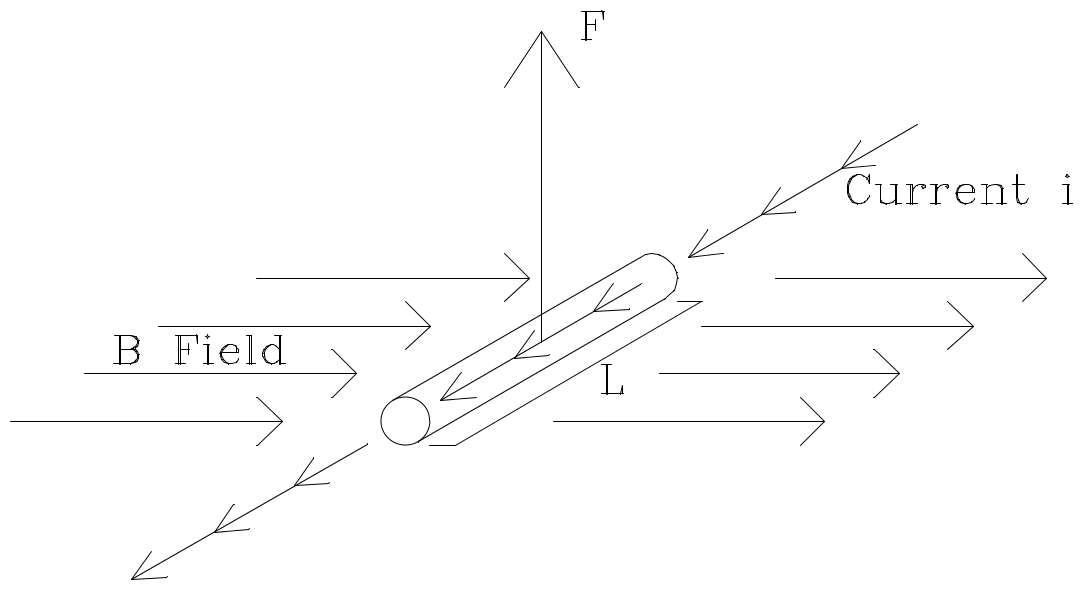
\includegraphics[width=0.6\textwidth]{./Exp4/pic/image1.png}
\caption{Force on a Current-carrying Wire}
\label{fig:force}
\end{figure}

\subsection{Induced EMF in a Coil}
According to Faraday's Law of induction, a changing magnetic flux through a coil induces an EMF (electromagnetic force) $\varepsilon$ given by
\begin{equation}
  \varepsilon=N\frac{\Delta \Phi}{\Delta t}
\end{equation}
where $\Phi = \int \vec{B} \cdot d \vec{A}$ is the flux of magnetic field $B$ through a coil of area $A$ and perpendicular to that area. $N$ is the number of turns in the search coil. For this experiment, the area of the coil is constant and the magnetic field is assumed to be uniform, so the average EMF is given by
\begin{equation}
  \varepsilon= -NA\frac{\Delta B}{\Delta t}
\end{equation}
The negative sign in Faraday's Law comes from the fact  that the EMF induced in the coil acts to oppose any change in the magnetic field. This is summarized as Lenz' Law. It is important to remember that EMF, despite being called a "force" is actually a potential and is measured in volts. Voltage will be induced as the coil enters and leaves magnetic field and its direction will be determined using Lenz' law.

\section{Procedure}
\subsection{Force on a Current-carrying Wire}

The experimental set-up is shown in Figure {\ref{fig:set-up}}. The horizontal magnetic field $B$ is produced in the air gap of a ``C-shaped'' iron electromagnet. The strength of $B$ is determined by the current in the magnet coils $I$, which is supplied by an adjustable low-voltage power supply.\myskip
\begin{figure}[h]
\centering
\includegraphics[width=0.8\textwidth]{./Exp4/pic/image2.png}
\caption{Experimental Set-up}
\label{fig:set-up}
\end{figure}

A more detailed drawing of the balance and electro-magnet arrangement is shown in Figure {\ref{fig:measureforce}}.

\begin{figure}[h]
\centering
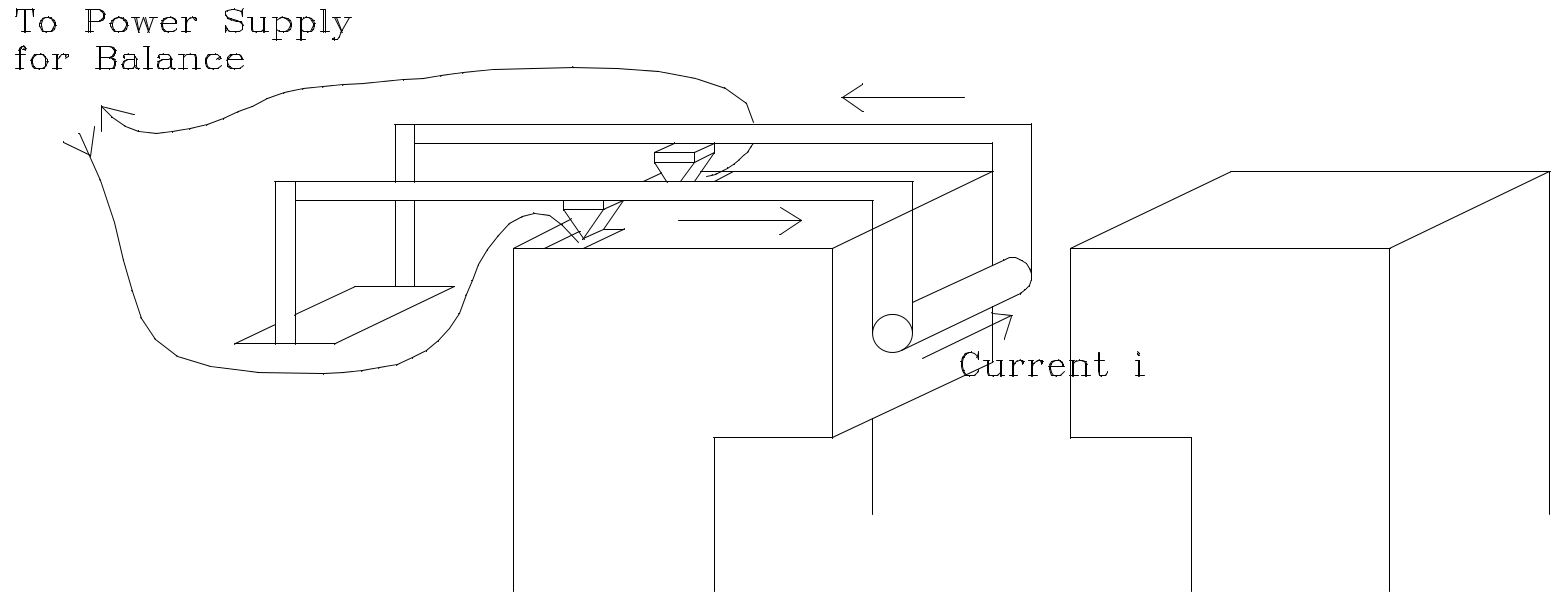
\includegraphics[width=0.8\textwidth]{./Exp4/pic/image3.png}
\caption{Setup of the Wire and Balance for Force Measurement}
\label{fig:measureforce}
\end{figure}

Note that the current $i$ through the horizontal conductor is supplied by a separate power supply. The current balance is constructed out of conducting and insulating materials such that current can enter through one side of the knife-edge fulcrum, flow through one side of the balance arm to the horizontal conductor, and then flow back through the other side of the balance arm and out through the other knife-edge. \myskip

The current $i$ in the balance is provided by the HP E3610A power supply, which can operate either in constant voltage or constant current mode. The voltage dial sets the \emph{maximum voltage} the device will supply to the circuit; the current dial likewise sets the \emph{maximum current}, and if the circuit tries to draw more current, the power supply will reduce the voltage until it reaches whatever value is needed to maintain the maximum current (by $V = IR$). \myskip

To use the power supply in constant current mode, begin with the current dial turned all the way down (counter-clockwise) and the voltage dial turned all the way up (clockwise). Set the range to 3 Amps, and connect the leads to the $+$ and $-$ terminals. You can now set the current to the desired level. Note that the digital meters on the power supply show the \emph{actual} voltage and current being supplied, so you will not normally see any current unless the leads are connected to a complete circuit. (If you want to set the current level without closing the circuit, you can hold in the CC Set button while you turn the current dial.) Once you close the circuit, the voltage adjusts automatically to maintain the constant current level, and the CC (Constant Current) indicator light should be on.

\begin{itemize}
  \item Set the current $I$ through the electromagnet at 5 amperes. Place a small number of weights on the balance and determine the value off $i$ necessary to reach equilibrium. Repeat for at least five different weights.

  \item With Microsoft Excel, plot the weight used to balance the scale vs. the balance current $i$. Include error bars.

  \item Draw a line of best fit and determine the slope with error using LINEST.

  \item From your slope, determine the magnetic field strength $B$ with error.

  \item Repeat the above steps (steps 1-4)  for two other magnet currents $I$ (for a total of three current data sets). You do not need to do error analysis for these measurements, but plot each of your results on the same graph.

  \item Draw a diagram similar to Figure \ref{fig:measureforce} and indicate the directions of $i$, $F$ and $B$ for your setup.

  \item Discuss potential sources of error.
\end{itemize}

\subsection{Induced EMF in a Coil}

\subsection{Experimental Apparatus}

A charge integrator (the Magnetic Field Module shown in Figure {\ref{fig:module}}) is used to measure the $\Delta Q$ produced by the EMF induced in the search coil. A capacitor in the module stores the charge $\Delta Q$, and the voltage across this capacitor (read on the external voltmeter shown) is proportional to $\Delta Q$. Therefore
\begin{equation}
  V=K\Delta Q=K\frac{N}{R}\Delta \Phi
\end{equation}
where $K$ is a constant that depends on the capacitance and gain of the integrator circuit. Instead of trying to calculate a value of $KN / R$ in terms of the components, it is more direct to calibrate the combination of the search coil and the integrator circuit by measuring $V$ for a known $\Delta \Phi$. This known magnetic flux can be created by passing a measured current $I_{\mathrm{sol}}$ through a long air-core solenoid of $n$ turns per meter and with a cross-sectional area of $A_{\mathrm{sol}}$ so that
\begin{equation}
  \Delta \Phi_{\mathrm{sol}}=B_{\mathrm{sol}}A_{\mathrm{sol}}=\mu_{0}nI_{\mathrm{sol}}A_{\mathrm{sol}}
\end{equation}
where $\mu_{0}$ is the permeability of free space ( $\mu_{0} = 4\pi \times 10^{-7}\, \mathrm{T}\cdot  \mathrm{m} / \mathrm{A} $).

\subsection{Procedure}
Connect the apparatus as shown in Figure {\ref{fig:module}}. Turn on the power supply. Before any measurements are made, depress the shorting switch, then release the shorting switch and turn the drift adjust control to minimize the drift in the output voltage as observed on your meter. The shorting switch must be used to discharge the integrating capacitor prior to each measurement. Also, the drift adjust setting should be checked occasionally. If the gain setting on the Magnetic Field Module is changed, the drift adjust control must be reset.\myskip

Magnetic field measurements are made by inserting or removing the search coil from the region containing the field to a field-free region or by leaving the search coil stationary and turning the field on or off.\myskip

Since the magnetic field in the large iron-core electromagnet is much greater than the field in an air-core solenoid, the Magnetic Field Module was designed with two gain settings. In the gain=100 position, the module is 100 times as sensitive as in the gain=1 position. For measuring fields generated by the air-core solenoid, set the gain at 100. For fields generated by the large electromagnet, set the gain at 1.\myskip

Connect the solenoid to the $+$ and $-$ terminals of the HP Power Supply. A three position (on-off-on) reversing switch is part of the solenoid circuit. Flip the switch to one of the on positions and adjust the power supply current such that two amperes is flowing through the solenoid.\myskip

Slide the search coil over the solenoid and, while holding the search coil at the center of the solenoid, discharge the Magnetic Field Module and then turn the current through the solenoid off using the three position switch (or turn the current from off to on). Take several readings and record the voltage on the integrator and the current through the solenoid. Then the result is
\begin{equation}
  V_{\mathrm{sol}}=100\cdot K\cdot \frac{N}{R}\cdot \Delta \Phi_{\mathrm{sol}}=100\cdot K\cdot \frac{N}{R}(\mu_{0}nI_{\mathrm{sol}})A_{\mathrm{sol}}
\label{eq:vsol}
\end{equation}

Now set the gain to 1 on the Magnetic Field Module, and readjust the drift controls. Set the current for the large electromagnet to 5 amps, and use the search coil to measure the resulting $B$. Move the search coil \emph{gently and smoothly} into the region of the magnetic field (do not move the coil hastily as you may damage it by striking against the magnet itself). Record $V_{\mathrm{mag}}$ . The corresponding equation is:
\begin{equation}
  V_{\mathrm{mag}}=K\cdot \frac{N}{R}A_{\mathrm{coil}}B_{\mathrm{mag}}
\label{eq:vmag}
\end{equation}

Combine the results of Eq({\ref{eq:vsol}}) and Eq({\ref{eq:vmag}}) to determine the value of $B$ for the large electromagnet when the current is 5 amps, and then do the same for the other magnet currents of 4, 3, and 2 amps. Compare these values for $B$ with those obtained in Part~I.

\chapter{$e/ m$ of The Electron}
\section{Intro}
The ``discovery'' of the electron by J. J. Thomson in 1897 refers to the experiment in which it was shown that ``cathode rays'' behave as beams of particles, all of which have the same ratio of charge to mass, $e/m$. Since that time, a number of experiments have been devised using electric and magnetic fields to precisely measure $e/m$ for the electron. When combined with the value of the electron's charge, which is measured in the Millikan Oil Drop Experiment, the determination of $e/m$ leads to an accurate value of the mass of the electron.\myskip

In the present experiment, electrons are emitted at a very low velocity from a heated filament, then accelerated through an electrical potential $V$ to a final velocity $v$, and finally bent in a circular path of radius $r$ in a magnetic field $B$. The entire process takes place in a sealed glass tube in which the path of the electrons can be directly observed. During its manufacture, the tube was evacuated, and a small amount of mercury was introduced before the tube was sealed off. As a result, there is mercury vapor in the tube. When electrons in the beam have sufficiently high kinetic energy ($10.4\,\mathrm{eV}$ or more), a small fraction of them will collide with and ionize mercury atoms in the vapor. Recombination of the mercury ions, accompanied by the emission of characteristic blue light, then occurs very near the point where the ionization took place. As a result, the path of the electron beam is visible to the naked eye. \myskip

The tube is set up so that the beam of electrons travels perpendicular to a uniform magnetic field $B$. $B$ is proportional to the current $I$ through a pair of large diameter coils (so-called ``Helmholtz Coils'') in which the coil separation is selected to produce optimum field uniformity near the center.

\section{Experimental Apparatus}
\subsection{The Sealed Glass Tube}
\begin{figure}[h]
\centering
\includegraphics[width=0.8\textwidth]{./Exp5/pic/image1.png}
\caption{Diagram of the Interior of the Sealed Glass Tube}
\label{fig:tube}
\end{figure}

Figure {\ref{fig:tube}} shows the filament surrounded by a small cylindrical plate. The filament is heated by passing a current directly through it. A variable positive potential difference of up to 100 volts is applied between the plate and the filament in order to accelerate the electrons emitted from the filament. Some of the accelerated electrons come out as a narrow beam through a slit in the side of the cylinder. The entire tube is located inside a set of coils, which produce a uniform magnetic field $B$ perpendicular to the electron beam. The magnitude of the field can be adjusted until the resultant circular path of the electron beam just reaches one of the measuring rods. These rods are located along a cross bar, which extends from the cylinder in a direction perpendicular to that in which the electron beam was emitted--i.e., along a diameter of the circular orbits.

\subsection{The Helmholtz Coils and Uniform Magnetic Field}
The magnetic field produced at the position of the electron beam by a current $I$ flowing through the coils must be computed. For a single turn of wire of radius $R$, the field on the axis at a distance $x$ from the plane of the loop is given by:
\begin{equation}
  B'=\frac{\mu_{0}R^{2}I}{2(R^2+x^2)^{3/2}}.
\end{equation}

For the arrangement in Figure {\ref{fig:coils}}, there are two loops with $N$ turns each, separated by a distance equal to the coil radius $R$. The coils contribute equally to the field at the center:
\begin{equation}
  B_{I}=\frac{\mu_{0}R^2NI}{\big[R^2+(R/2)^2\big]^{3/2}}=\frac{4\pi\times 10^{-7}NI}{R(1+\frac{1}{4})^{3/2}}=\mathrm{constant}\times I\, \mathrm{Tesla}
\label{eq:bi}
\end{equation}
where $N = 72$ is the number of turns of each coil and $R = 33\, \mathrm{cm}$ is the radius of the coils used.\myskip
\begin{figure}[h]
\centering
\includegraphics[width=0.8\textwidth]{./Exp5/pic/image2.png}
\caption{Helmholtz coils used to produce a uniform magnetic field.}
\label{fig:coils}
\end{figure}

This arrangement, called a pair of \textbf{Helmholtz coils}, yields a remarkably uniform field in the region at the center.\myskip

The net field $B$ in which the electrons move is not $B_I$ alone, however. We also feel some of the Earth's own magnetic field, $B_E$. If the equipment is oriented such that these two fields, $B_I$ and $B_E$ are parallel, then the net field will be the sum of the two parts. And if $B_I$ is set to be in the opposite direction to $B_E$, then the we have
\begin{equation}
  B=B_{I}-B_{e}.
\label{eq:b}
\end{equation}

\subsection{The Trajectories of the Electrons in the Glass Tube}
If an electron of charge $e$ and mass $m$ starts nearly from rest and is accelerated through a potential difference $V$ to a final velocity $v$, then
\begin{equation}
  \frac{1}{2}mv^2=eV\quad \mathrm{or}\quad \frac{e}{m}=\frac{v^2}{2V}
\label{eq:ev}
\end{equation}

If the electron then enters a uniform magnetic field $B$ which is perpendicular to its velocity, it will move in a circular orbit of radius $r$, where
\begin{equation}
  \frac{mv^2}{r}=evB\quad\mathrm{or}\quad \frac{e}{m}=\frac{v}{Br}
\label{eq:eb}
\end{equation}

If it were possible to measure the velocity directly, then $e/m$ could be determined by measurements of either the electric or magnetic field alone. Since a direct measurement of $v$ is not feasible in this experiment, $e/m$ can best be determined from the combination of electric and magnetic fields used. Specifically, by eliminating $v$ from equations ({\ref{eq:ev}}) and ({\ref{eq:eb}}), $e/m$ can be expressed directly in terms of $V$, $B$, and $r$.\myskip

Instead of determining $e/m$ from a single measurement of $r$ for given values of $V$ and $B$, however, it is preferable to measure the variation of $r$ with $B$ (or $I$) at fixed values of $V$. In particular, the data can be presented in convenient form by plotting the \textbf{curvature} $1/r$ as a linear function of $I$.
\begin{equation}
  \frac{1}{r}=\sqrt{\frac{e}{m}\frac{1}{2V}}B_{I}-\sqrt{\frac{e}{m}\frac{1}{2V}}B_{e}
\label{eq:r}
\end{equation}

Derive ({\ref{eq:r}}) from ({\ref{eq:b}}), ({\ref{eq:ev}}), and ({\ref{eq:eb}}) for your report \underline{before} coming to laboratory.\myskip

Note that equations ({\ref{eq:ev}}), ({\ref{eq:eb}}), and ({\ref{eq:r}}) apply strictly only to electrons with trajectories on the \emph{outside edge} of the beam -- i.e., the most energetic electrons. There are two reasons why some electrons in the beam will have less energy:
\begin{enumerate}
\item There is a small potential difference across the filament caused by the heating current. Only electrons leaving the negative end of the filament are accelerated through the whole potential difference $V$.
\item Some of the electrons in the beam will lose energy through collisions with mercury atoms.
\end{enumerate}

\section{Procedure}
\subsection{Orientation of the Coil and Tube Setup}

For reasons already explained, we would like to orient the Helmholtz coils such that their axes are parallel to the ambient magnetic field.\myskip

\emph{Please exercise extreme care in the following section as you align the Helmholtz coils: the cathode ray tube is very delicate and may break if the coil support is not very firmly secured and falls.  It is recommended that two people handle the coil frame at all times while the coils are being aligned.  Also take care not to touch the dip needle, which is easily bent.}\myskip

In order to align the coils so that their axis is aligned with the ambient magnetic field proceed as follows:
\begin{enumerate}
    \item With the coils in the horizontal position, rotate the horizontal arm of the dip needle support so that the needle itself and the plastic protractor are horizontal.  Avoid touching the needle or plastic protractor, and instead turn the arm using the attached lever.
    \item Allow the compass needle to come to a rest.  It is now pointing in the direction of the horizontal component of the ambient field.
    \item Rotate the entire frame by turning the base, until the compass needle is aligned along the $90^\circ$-$270^\circ$ line on the protractor.  The horizontal axis of the cathode ray tube (coaxial with the metal rod) is now aligned with the horizontal component of the ambient field.
    \item Rotate the horizontal arm of the dip needle support so that the needle itself and the plastic protractor are now in a vertical plane.  Avoid touching the needle or plastic protractor, and instead turn the arm using the attached lever.
    \item Allow the needle to come to a rest.  It is now pointing in the direction of the ambient field.
    \item Loosen the wingnut and \textbf{gently} raise one side of the coils.  You want to increase the angle until the dip needle is aligned along the $0^\circ$-$180^\circ$ line on the protractor.  \textbf{Hold the wooden frame rather than the coils as you raise the setup}.
    \item Securely \textbf{tighten the wingnut so that the coils remain in position}.  One person should be supporting the frame while a second person tightens the wingnut.
    \item The coil axis should now be aligned (coaxial) with the ambient magnetic field.
\end{enumerate}

\subsection{Preliminary Adjustments}
The supplies and controls for the Helmholtz coils and the filament are permanently wired on a board and are designed to minimize the possibility of damage to the tube or coils. Locate each control, and note the qualitative effects observed when the control is varied. In particular:
\begin{enumerate}
\item Figure {\ref{fig:tube}} shows that the filament and its associated lead wires form a small loop. Since a $4\,\mathrm{amp}$ current is required to heat the filament, this loop creates its own measurable magnetic field. The filament coil reversing switch permits you to study the effect of this field. To minimize this effect, rotate the entire tube slightly in its mounting so the electrons come out parallel to the plane of the coils.
\item Note the direction of the coil current for each position of its reversing switch by using the dip needle to check the direction of the resultant field. Knowing the field direction, check the sign of the charge of the particles in the deflected beam. Also, determine whether the earth's field adds to or subtracts from the coil field.
\end{enumerate}

\subsection{Measurement of $e/m$}
With the accelerating voltage at some intermediate value, you may adjust the current in the Helmholtz coils so that the outside edge of the beam strikes the outside edge of each bar in turn.
\begin{enumerate}
  \item Measure field current as a function of radius for the highest voltage $V$ which allows you to adjust the beam with respect to all five bars. You can find this voltage by first setting the Helmholtz current to its maximum value and then adjusting the accelerating voltage until electrons pass through the shortest diameter bar.\\ \\

  The tube manufacturer supplies the following values for the \emph{diameters} from the filament to the \emph{outside} of each bar in succession:
  \begin{gather*}
  6.48\,\textrm{cm},\quad 7.75\,\textrm{cm},\quad 9.02\,\textrm{cm},\quad 10.30\,\textrm{cm},\quad 11.54\,\textrm{cm}
  \end{gather*}

  \item For one of your five measurements, test the reproducibility of the current setting as an aid to error analysis. Do this by turning the power supply off and on again. Then readjust the current until the electrons pass through the relevant bar. Do this six times and use the 2/3 method to determine an appropriate uncertainty in field current.

  \item With Microsoft Excel, plot $1/r$ vs. field current $I$ with error bars and draw a best fit line. Calculate the slope of your line and find the error using LINEST.

  \item Using equations ({\ref{eq:r}}) and ({\ref{eq:bi}}), determine $e/m$ from the slope of your best-fit line with error.

  \item Does your calculated $e/m$ value agree with the accepted value within error? The accepted value is $1.758 \times 10^{11}\, \mathrm{coulombs} / \mathrm{kg}$.

  \item Calculate the actual maximum velocity of the electrons in your beam with error found by propagating uncertainties in $e/m$.

  \item Use the intercept of your best-fit line to calculate the strength of the Earth's magnetic field $B_e$ with error.

  \item Discuss the main sources of error in measuring $\frac{e}{m}$ in this experiment.
\end{enumerate}

%\chapter{$e/ m$ of The Electron}
\section{General Discussion}
The ``discovery'' of the electron by J. J. Thomson in 1897 refers to the experiment in which it was shown that ``cathode rays'' behave as beams of particles, all of which have the same ratio of charge to mass, $e/m$. Since that time, a number of methods have been devised for using electric and magnetic fields to make a precise measurement of $e/m$ for the electron. When combined with the value of the electron's charge, which is measured in the Millikan Oil Drop Experiment, the determination of $e/m$ leads to an accurate value of the mass of the electron. In the present experiment, electrons are emitted at a very low velocity from a heated filament, then accelerated through an electrical potential $V$ to a final velocity $v$, and finally bent in a circular path of radius $r$ in a magnetic field $B$. The entire process takes place in a sealed glass tube in which the path of the electrons can be directly observed. During its manufacture, the tube was evacuated, and a small amount of mercury was introduced before the tube was sealed off. As a result, there is mercury vapor in the tube. When electrons in the beam have sufficiently high kinetic energy ($10.4\,\mathrm{eV}$ or more), a small fraction of them will collide with and ionize mercury atoms in the vapor. Recombination of the mercury ions, accompanied by the emission of characteristic blue light, then occurs very near the point where the ionization took place. As a result, the path of the electron beam is visible to the naked eye. \myskip

The tube is set up so that the beam of electrons travels perpendicular to a uniform magnetic field $B$. $B$ is proportional to the current $I$ through a pair of large diameter coils (so-called ``Helmholtz Coils'') in which the coil separation is selected to produce optimum field uniformity near the center.

\section{Experimental Apparatus}
\subsection{The Sealed Glass Tube}
\begin{figure}[h]
\centering
\includegraphics[width=0.8\textwidth]{./Exp6/pic/image1.png}
\caption{Diagram of the Interior of the Sealed Glass Tube}
\label{fig:tube}
\end{figure} 

Figure {\ref{fig:tube}} shows the filament surrounded by a small cylindrical plate. The filament is heated by passing a current directly through it. A variable positive potential difference of up to 100 volts is applied between the plate and the filament in order to accelerate the electrons emitted from the filament. Some of the accelerated electrons come out as a narrow beam through a slit in the side of the cylinder. The entire tube is located inside a set of coils, which produce a uniform magnetic field $B$ perpendicular to the electron beam. The magnitude of the field can be adjusted until the resultant circular path of the electron beam just reaches one of the measuring rods. These rods are located along a cross bar, which extends from the cylinder in a direction perpendicular to that in which the electron beam was emitted--i.e., along a diameter of the circular orbits. 

\subsection{The Helmholtz Coils and Uniform Magnetic Field}
The magnetic field produced at the position of the electron beam by a current $I$ flowing through the coils must be computed. For a single turn of wire of radius $R$, the field on the axis at a distance $x$ from the plane of the loop is given by:
\begin{equation}
  B'=\frac{\mu_{0}R^{2}I}{2(R^2+x^2)^{3/2}}.
\end{equation}

For the arrangement in Figure {\ref{fig:coils}}, there are two loops with $N$ turns each, separated by a distance equal to the coil radius $R$. The coils contribute equally to the field at the center:
\begin{equation}
  B_{I}=\frac{\mu_{0}R^2NI}{\big[R^2+(R/2)^2\big]^{3/2}}=\frac{4\pi\times 10^{-7}NI}{R(1+\frac{1}{4})^{3/2}}=\mathrm{constant}\times I\, \mathrm{Tesla}
\end{equation}
where $N = 72$ is the number of turns of each coil and $R = 33\, \mathrm{cm}$ is the radius of the coils used.\myskip
\begin{figure}[h]
\centering
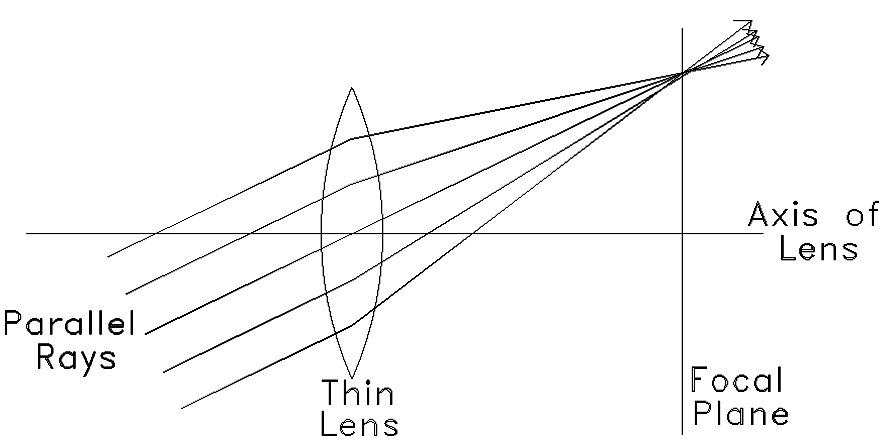
\includegraphics[width=0.8\textwidth]{./Exp6/pic/image2.png}
\caption{Helmholtz coils used to produce a uniform magnetic field.}
\label{fig:coils}
\end{figure} 

This arrangement, called a pair of \textbf{Helmholtz coils}, yields a remarkably uniform field in the region at the center.\myskip

The net field $B$ in which the electrons move is not $B_I$ alone, but the resultant of the earth's field $B_e$ and $B_I$ . If the equipment is oriented so that the field of the Helmholtz coils is parallel to that of the earth, and if the current through the coils causes $B_I$ to be directed opposite to $B_e$ , then
\begin{equation}
  B=B_{I}-B_{e}
\label{eq:b}
\end{equation}

\subsection{The Trajectories of the Electrons in the Glass Tube}
If an electron of charge $e$ and mass $m$ starts nearly from rest and is accelerated through a potential difference $V$ to a final velocity $v$, then
\begin{equation}
  \frac{1}{2}mv^2=eV\quad \mathrm{or}\quad \frac{e}{m}=\frac{v^2}{2V}
\label{eq:ev}
\end{equation}

If the electron then enters a uniform magnetic field $B$ which is perpendicular to its velocity, it will move in a circular orbit of radius $r$, where
\begin{equation}
  \frac{mv^2}{r}=evB\quad\mathrm{or}\quad \frac{e}{m}=\frac{v}{Br}
\label{eq:eb}
\end{equation}

If it were possible to measure the velocity directly, then $e/m$ could be determined by measurements of either the electric or magnetic field alone. Since a direct measurement of $v$ is not feasible in this experiment, $e/m$ can be determined from the combination of electric and magnetic fields used. Specifically, by eliminating $v$ from equations ({\ref{eq:ev}}) and ({\ref{eq:eb}}), $e/m$ can be expressed directly in terms of $V$, $B$, and $r$.\myskip

Instead of determining $e/m$ from a single measurement of $r$ for given values of $V$ and $B$, however, it is preferable to measure the variation of $r$ with $B$ (or $I$) at fixed values of $V$. In particular, the data can be presented in convenient form by plotting the \textbf{curvature} $1/r$ as a linear function of $I$.
\begin{equation}
  \frac{1}{r}=\sqrt{\frac{e}{m}\frac{1}{2V}}B_{I}-\sqrt{\frac{e}{m}\frac{1}{2V}}B_{e}
\label{eq:r}
\end{equation}

Derive ({\ref{eq:r}}) from ({\ref{eq:b}}), ({\ref{eq:ev}}), and ({\ref{eq:eb}}) for your report \underline{before} coming to laboratory.\myskip

Note that equations ({\ref{eq:ev}}), ({\ref{eq:eb}}), and ({\ref{eq:r}}) apply strictly only to electrons with trajectories on the \emph{outside edge} of the beam -- i.e., the most energetic electrons. There are two reasons why some electrons in the beam will have less energy:
\begin{enumerate}
\item There is a small potential difference across the filament caused by the heating current. Only electrons leaving the negative end of the filament are accelerated through the whole potential difference $V$.
\item Some of the electrons in the beam will lose energy through collisions with mercury atoms.
\end{enumerate}

\section{Procedure}
\subsection{Orientation of the Coil and Tube Setup}

For reasons already explained, we would like to orient the Helmholtz coils such that their axes are parallel to the ambient magnetic field.\myskip

\emph{Please exercise extreme care in the following section as you align the Helmholtz coils: the cathode ray tube is very delicate and may break if the coil support is not very firmly secured and falls.  It is recommended that two people handle the coil frame at all times while the coils are being aligned.  Also take care not to touch the dip needle, which is easily bent.}\myskip

In order to align the coils so that their axis is aligned with the ambient magnetic field proceed as follows:
\begin{itemize}
    \item With the coils in the horizontal position, rotate the horizontal arm of the dip needle support so that the needle itself and the plastic protractor are horizontal.  Avoid touching the needle or plastic protractor, and instead turn the arm using the attached lever.
    \item Allow the compass needle to come to a rest.  It is now pointing in the direction of the horizontal component of the ambient field.
    \item Rotate the entire frame by turning the base, until the compass needle is aligned along the $90^\circ$-$270^\circ$ line on the protractor.  The horizontal axis of the cathode ray tube (coaxial with the metal rod) is now aligned with the horizontal component of the ambient field.
    \item Rotate the horizontal arm of the dip needle support so that the needle itself and the plastic protractor are now in a vertical plane.  Avoid touching the needle or plastic protractor, and instead turn the arm using the attached lever.
    \item Allow the needle to come to a rest.  It is now pointing in the direction of the ambient field.
    \item Loosen the wingnut and \textbf{gently} raise one side of the coils.  You want to increase the angle until the dip needle is aligned along the $0^\circ$-$180^\circ$ line on the protractor.  \textbf{Hold the wooden frame rather than the coils as you raise the setup}.
    \item Securely \textbf{tighten the wingnut so that the coils remain in position}.  One person should be supporting the frame while a second person tightens the wingnut.
    \item The coil axis should now be aligned (coaxial) with the ambient magnetic field.
\end{itemize}

\subsection{Preliminary Adjustments}
The supplies and controls for the Helmholtz coils and the filament are permanently wired on a board and are designed to minimize the possibility of damage to the tube or coils. Locate each control, and note the qualitative effects observed when the control is varied. In particular:
\begin{enumerate}[(a)]
\item Figure {\ref{fig:tube}} shows that the filament and its associated lead wires form a small loop. Since a $4\,\mathrm{amp}$ current is required to heat the filament, this loop creates a measurable field. The filament coil reversing switch permits you to study the effect of this field. The effect can be minimized in the experiment by rotating the tube slightly in its mounting so that the electrons come out parallel to the plane of the coils.
\item Note the direction of the coil current for each position of its reversing switch by using the dip needle to check the direction of the resultant field. Knowing the field direction, check the sign of the charge of the particles in the deflected beam. Also, determine whether the earth's field adds to or subtracts from the coil field.
\item The beam will have a slight curvature in the earth's field when the coil current is zero. Make a preliminary measurement of the earth's field by adjusting the coil current to remove this curvature. The special Meter Switch and low current meter ($200\, \mathrm{mA}$) will enable you to measure the relatively small current needed, and the straight line trajectory can be checked by comparison with the light emitted from the filament.
\end{enumerate}

\subsection{Measurement of the Circular Orbits}
With the accelerating voltage at an intermediate value, the current in the Helmholtz coils can be adjusted so that the outside edge of the beam strikes the outside edge of each bar in turn. Measure field current as a function of radius for the highest voltage $V$ which allows you to adjust the beam with respect to all five bars.\myskip

For one measurement, test the reproducibility of the current setting as an aid to error analysis. The tube manufacturer supplies the following values for the \emph{diameters} from the filament to the \emph{outside} of each bar in succession:
\begin{gather*}
6.48\,\textrm{cm},\quad 7.75\,\textrm{cm},\quad 9.02\,\textrm{cm},\quad 10.30\,\textrm{cm},\quad 11.54\,\textrm{cm}
\end{gather*}

\subsection{Calculations}
Plot a graph of $1/r$ versus $I$, and draw the straight line that gives a best fit to the five measured points. Use equation ({\ref{eq:r}}) to calculate $e/m$ from the slope of this line. Write your report up to this point and then proceed to the following:

\subsection{Further Considerations}
\begin{enumerate}[(a)]
\item Calculate the percentage difference between your value of $e/m$ and the accepted value which is $1.758 \times 10^{11}\, \mathrm{coulombs} / \mathrm{kg}$. What do you think is your largest source of error? Can you account for this much error by a numerical estimate?
\item Calculate the actual maximum velocity of the electrons in your beam.
\item Make another run with a lower accelerating voltage. Do you find a consistent value of $e/m$?
\item Compare the intercept of your graph with the value of coil current you obtained by balancing the earth's field. If these numbers are not roughly the same, you may have made an error. Note that this current is not an important number, but it makes a good check on your technique. Physicists frequently check the consistency of their data by computing numbers which they do not ``need''.
\item Calculate the actual value of $B_e$ .
\item Test the maximum error in your readings which could be caused by a change in the field of the nearest neighboring coil.
\end{enumerate}

%\chapter{Polarization and Interference}
\section{Introduction}
You have already investigated some wave properties in last semester's Experiment 9. This lab will address three concepts of waves: polarization, interference, and diffraction. We will conduct this experiment with light, but the general concepts apply to many other waves as well.

\section{Theory}
\subsection{Polarization}
Polarization occurs only in transverse waves\footnote{Examples of transverse waves are oscillations on a string, water waves, or the electromagnetic radiation we treat here. Sometimes you may also hear the term polarization used in the context of transverse- and longitudinal polarization.}. By definition, the oscillation is perpendicular to the direction of wave propagation in a transverse wave. Since in three-dimensional space there are three independent dimensions, there are two possible perpendicular directions needed to describe any oscillatory motion perpendicular to the direction of motion. If you think about a transverse wave in a string, the oscillation could be up-and-down or left-and-right, while the wave front propagates forward along the string. The two independent and perpendicular directions are called the two polarization states. (Or in coordinates, if a wave propagates along the $z$-axis, there are two polarizations perpendicular to the wave motion--one along the $x$-axis and one along the $y$-axis.) Polarization cannot occur in longitudinal waves because the direction of oscillation has only one possibility, along the direction of motion.\myskip

You may argue that you can make oscillations happen on a string in more than just the two directions described above--and you are right! For example, you can make oscillations diagonally from the upper left to the lower right or you can even make circular oscillations by moving your hand continuously in a circle, producing a corkscrew pattern along the string\footnote{This wave is sometimes called left- or right- circular polarization.}. But no matter which wave you make, the oscillations can always be represented as two superimposed waves with displacements along the two mutually perpendicular polarization axes. Any vector can always be described by decomposing it into its $x$- and $y$- components. Here, the relevant vector is the oscillating displacement from the $z$-axis. The amplitudes of the resolved $x$ and $y$ components indicate how much of the wave is in each polarization state.\myskip

For electromagnetic radiation, the oscillating quantities are the electric (and magnetic) fields. These undulate perpendicular to the direction of the wave. Like waves in a string, electromagnetic waves are transverse waves and have polarization properties. The polarization state describes the axis along which the electric field in the wave oscillates. Visible light is electromagnetic radiation in a particular frequency-wavelength regime, with large frequency of oscillation ($\sim 10^{15}\,\mathrm{Hz}$) and small wavelength ($\sim 0.5\times 10^{-6}\, \mathrm{m}$).\myskip

\subsection{Polarizer}
Usually light is produced (e.g. incandescent light from a candle or a light bulb) by hot electrons and atoms, which are moving or are oriented in random directions, so that the wave is \textbf{unpolarized}. This means that the electric field associated with the wave oscillates in random directions (though always at right angles to the direction of the propagation of the light). So there is no favored direction for polarization. It is as if you were moving your hand in random directions at the end of a string. Note that this is very different from the cases of waves in a string described above. Even in circular polarization the oscillations were not random.
\begin{figure}[h]
\centering
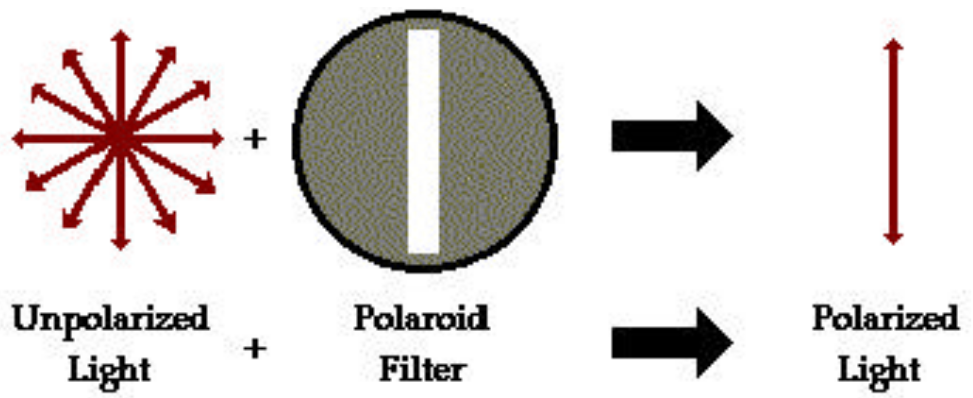
\includegraphics[width=0.5\textwidth]{./Exp7/pic/image1.png}
\caption{Polarization Filter and Creation of Polarized Light}
\label{fig:creation}
\end{figure} 

A polarization filter, shown in Figure {\ref{fig:creation}}, is a device with a specified direction, called the polarization axis. The filter absorbs all the wave's incoming electric field perpendicular to the polarization axis and transmits the electric field parallel to the polarization axis. So no matter what the polarization of the light shining into a polarizer might be, the light coming out of the polarizer is always polarized in the direction specified by the polarization axis\footnote{Such light is called linearly polarized light.}. An unpolarized wave just prior to the polarizer has an electric field ($\mathbf{E}$) pointing randomly in all directions perpendicular to the wave direction, as shown in Figure {\ref{fig:detection}}. The polarized wave after the polarizer has only half the energy content, and the $\mathbf{E}$-field is oscillating solely along the polarization axis. This electric field has the same value as the component along that axis just before the polarizer.
\begin{figure}[h]
\centering
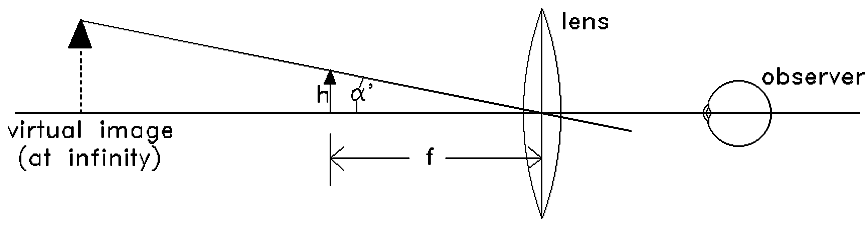
\includegraphics[width=0.8\textwidth]{./Exp7/pic/image2.png}
\caption{Detection of Polarized Light}
\label{fig:detection}
\end{figure} 

\subsection{Interference--The Double Slit}
As you've learned in class, Young's double slit experiment is a demonstration of interference and diffraction. A double slit, as illustrated in Figure {\ref{fig:double}}, permits what remains of anincoming wave (from the left) to travel to a distant screen (to the right) along two different paths with different lengths. The light waves from the two slits interfere, resulting in an interference pattern of bright (constructive) and dim (destructive) patches as viewed on the screen. Let's see how the double slit works using Figure {\ref{fig:double}}.
\begin{figure}[h]
\centering
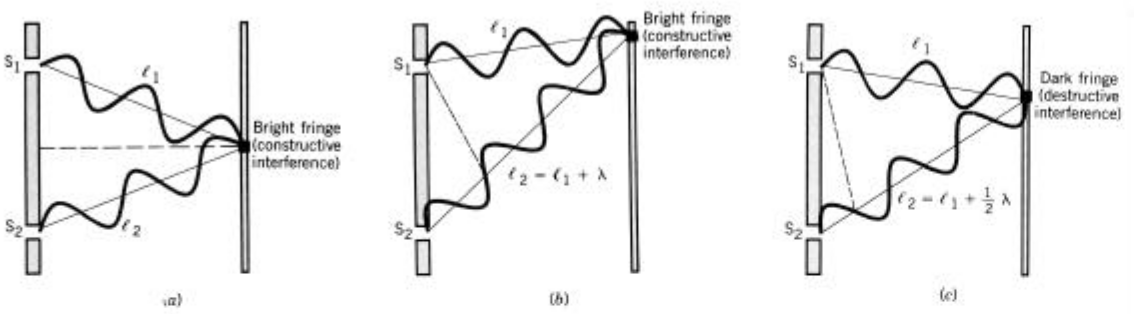
\includegraphics[width=0.8\textwidth]{./Exp7/pic/image3.png}
\caption{Young's Double Slit Experiment}
\label{fig:double}
\end{figure} 

We shine light from the left onto the double slit, which allows two light waves to propagate from the two slits. Straight-ahead they will always be in phase since they travel the same distance to the screen. But when the two waves propagate at an angle $\theta$, they cover different distances to reach a specific point on the screen. (We assume that the two rays are parallel, a good approximation since the screen is effectively infinitely far away compared to the distance between the two slits.)\myskip
\begin{figure}[h]
\centering
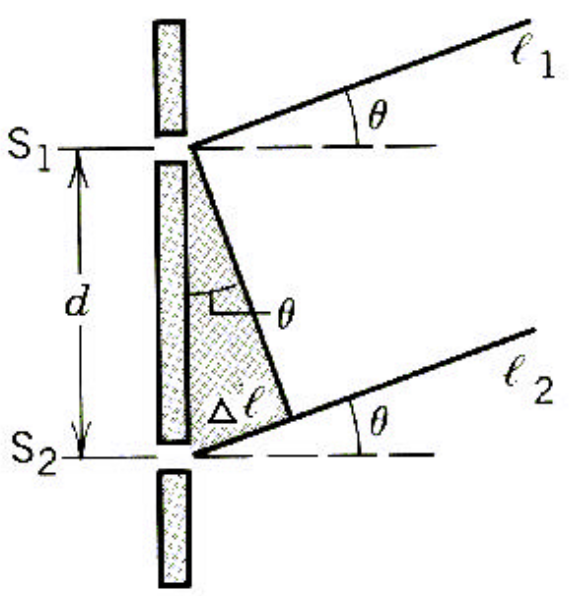
\includegraphics[width=0.3\textwidth]{./Exp7/pic/image4.png}
\caption{Geometry of the Double Slit}
\label{fig:geometry}
\end{figure} 

As you can convince yourself by applying the rules of trigonometry to the triangle in Figure {\ref{fig:geometry}}, the difference in path ($\Delta l$) between the two rays is, for slit separation, $d$,
\begin{equation}
  \Delta l =d\sin\theta
\end{equation}

So what quantitatively determines a point of maximum intensity on the screen? Maximum intensity occurs if the two waves are precisely in phase at that point on the screen. This follows from what you learned about constructive and destructive interference in the lab on standing waves. As you saw, two waves can add up constructively or destructively. In the case of maximal constructive interference, the waves combine at the screen so that a crest on one wave coincides with a crest on the other wave and a trough coincides with a trough. In the case of maximal destructive interference, the waves combine so that a crest on one wave coincides with a trough on the other wave. \myskip

The waves will be in phase when they meet at the screen if the path difference between the two waves is an exact number of wavelengths, $m$, where $m$ is an integer called the order of the maximum. This requirement, expressed mathematically, is
\begin{equation}
  \Delta l =m\lambda
\end{equation}

Note that if $m=0$, there is no difference in the path lengths, resulting in a maximum straight ahead, $\theta=0$, as shown in Figure {\ref{fig:interference}}. Subsequent maxima occur for subsequent positive and negative integers, $m=\pm 1, \pm 2, \pm 3, \dots$. \myskip 

Combining the two equations for $\Delta l$, we get for the specific angles, $\theta_{m}$ , that give maximal constructive interference:
\begin{equation}
  d\sin \theta_{m}=m\lambda
\end{equation}

If we know the order $m$ of a particular maximum, we can determine the wavelength of the light incident on the double slit by measuring the angle of the maximum on the screen. Conversely, we can determine the order of a particular maximum, $m$, from the wavelength of the light and the angle.
\begin{figure}[h]
\centering
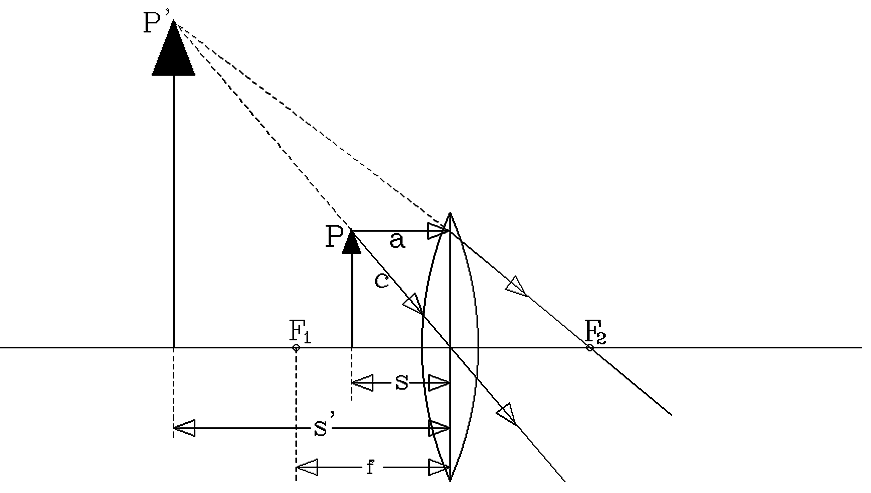
\includegraphics[width=0.6\textwidth]{./Exp7/pic/image5.png}
\caption{Interference of Light Coming from Two Small Slits}
\label{fig:interference}
\end{figure} 

\subsection{Intensity of the Double-Slit Maxima}
You will soon note that the intensities for subsequent maxima are different. What causes this? Just as the double slit creates an interference pattern, each single slit creates a diffraction pattern due to interference from waves coming from different parts of a single slit as described in section 39-6 of the lecture course text\footnote{Sears, Zemansky, and Young, \textbf{College Physics \engordnumber{7} edition}, Addison-Wesley, p. 903-906.}. This occurs because each individual slit has a finite width. The overall (more realistic) pattern shown in figure {\ref{fig:intensity}} is a superposition of the single slit and double slit interference patterns. The narrow spikes (of interest for this experiment) are due to the double slit interference and the envelope, or large-scale pattern, is due to the single slit diffraction caused by each slit.
\begin{figure}[h]
\centering
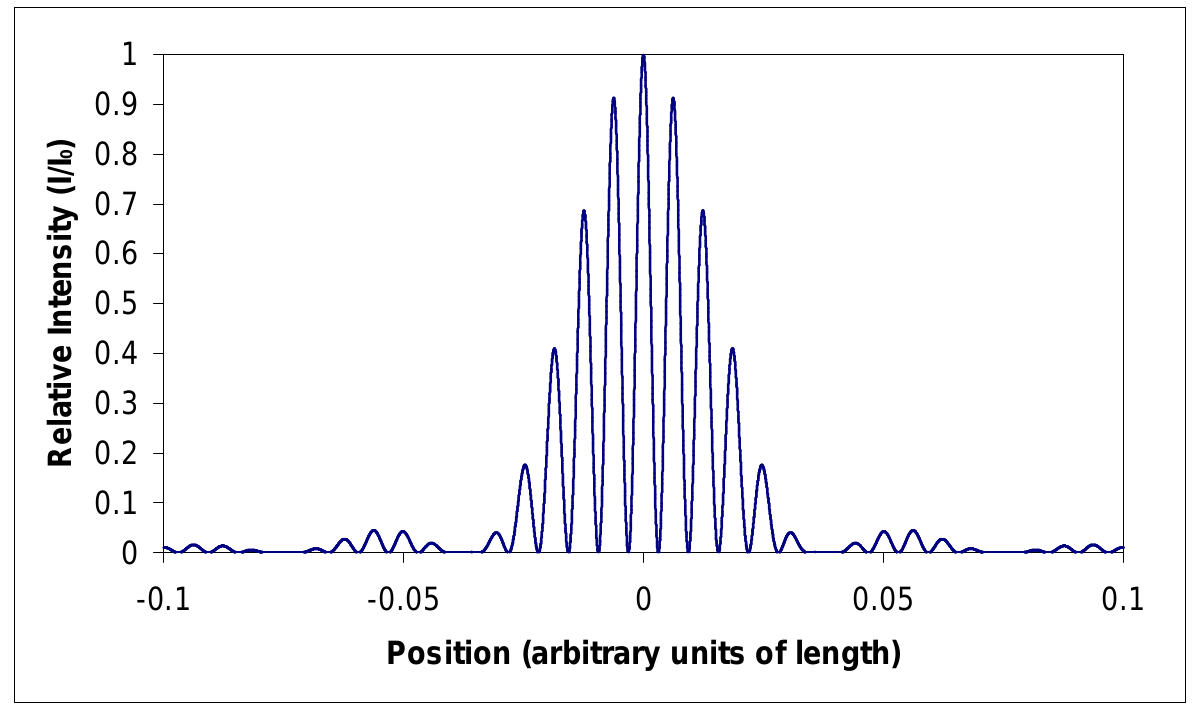
\includegraphics[width=0.8\textwidth]{./Exp7/pic/image6.png}
\caption{Intensity Pattern of the Double Slit. The Many Peaks of the Narrow Spikes Correspond to the Maxima in $d\sin\theta_{m}=m\lambda$}
\label{fig:intensity}
\end{figure} 

\subsection{Light from a Laser}
In the double slit experiment we use a laser as the light source. Laser light differs from incandescent or fluorescent light in two important ways. First, lasers emit intense light of a single wavelength or frequency (monochromatic). Second, laser light is coherent, meaning that all light waves are in phase.\myskip

 Let's illustrate the differences between coherent and incoherent light through a simple familiar example. Contrast a crowd of people cramming the city streets during rush hour with a regiment of soldiers at a parade. In the midtown crowd, even if everybody were to step at the same frequency (which they don't!), each pedestrian's steps are independent of what others are doing. But soldiers at a parade move in step, or in phase, with a similar frequency, taking their steps at exactly the same time. Laser light is like the (coherent) soldiers at a parade, whereas light from a light bulb is like the (incoherent) civilian crowd at Times Square.\myskip

Although incandescent light sources\footnote{This is easily visible in the colors produced by soap bubbles.} can produce diffraction and interference patterns, a laser is better suited to illustrate coherent phenomena.

\section{Experiments}
\subsection{Polarization}
Suppose a wave has linearly polarized light characterized by an electric field vector, $\mathbf{E}_{0}$, at an angle, $\phi$ , relative to the direction of a polarizer. The electric field that is transmitted through the polarizer is $\mathbf{E}=\mathbf{E}_{0}\cos\phi$, the component that was not absorbed. Since the energy intensity in the wave is proportional to $\mathbf{E}^2$, then the intensity passing through two polarizers will be proportional to the square of the cosine of the angle φ between the two polarizing axes.\footnote{This relation is sometimes referred to as Malus' Law, after Etienne Malus, who also discovered the polarization of reflected light in the early nineteenth century.}
\begin{equation}
  I=I_{\mathrm{max}}\cos^2\phi
\label{eq:i}
\end{equation}

In this experiment, we use an incandescent unpolarized light source and then polarize it by first passing it through a polarizer. The electric field vector $\mathbf{E}_{0}$ will then point along the same direction as the polarizing axis of the first polarizer. As the now polarized light falls on the second polarizer, only the component of $\mathbf{E}_{0}$ along the polarizing axis of the second polarizer will make it through unaffected. \myskip

As figure {\ref{fig:polarized}} illustrates, an electric field strength of only $\mathbf{E}_{0}\cos\phi$ will make it through the second polarizer, so that the new intensity will be given by Equation {\ref{eq:i}} above. A human eye or a photometer can detect this change in light intensity.
\begin{figure}[h]
\centering
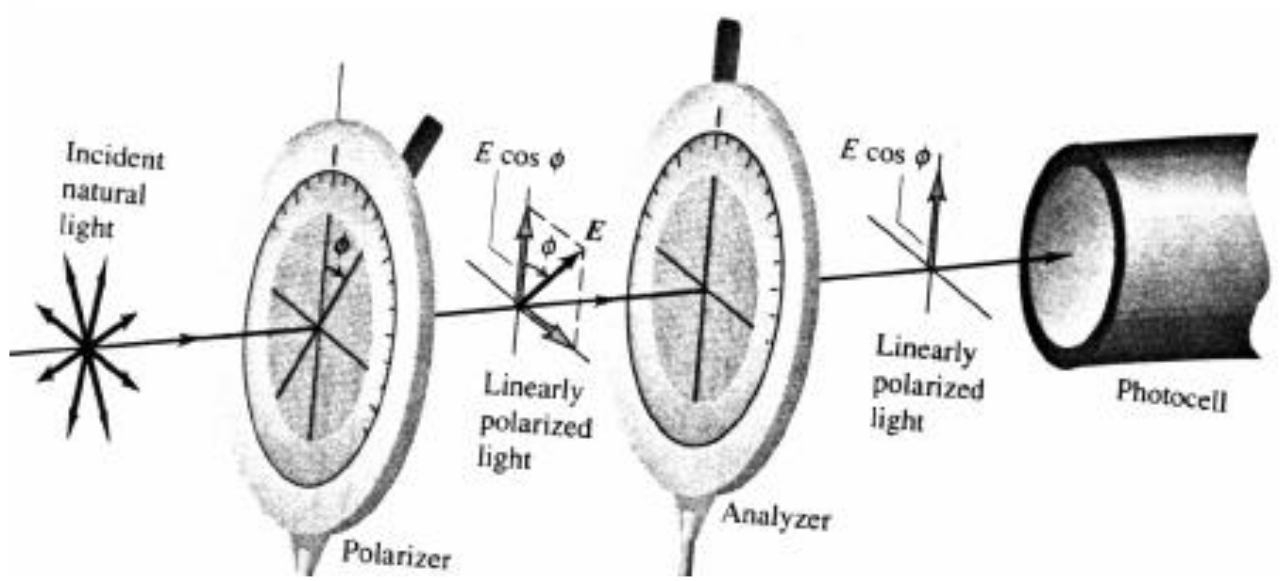
\includegraphics[width=0.8\textwidth]{./Exp7/pic/image7.png}
\caption{Creation and Detection of Polarized Light}
\label{fig:polarized}
\end{figure} 

\subsection{Double Slit}
In this part of the experiment we use a laser instead of incandescent light source. Laser light shines onto a double slit, which produces an interference pattern of bright and dark lines on the wall or a piece of paper beyond the double slit. \myskip

We know that the angle, $\theta_{m}$, at which the $m^{\mathrm{th}}$ order bright spot appears is given by
\begin{equation}
  d\sin\theta_{m}=m\lambda
\end{equation}

For small $\theta_{m}$ (in radians), the approximation $\sin\theta \approx \tan\theta \approx \theta$ is valid\footnote{See for yourself by punching $\sin 0.1$ and $\tan 0.1$ into your calculator (using radiant measure)!}. So on a screen far away from the double slit, we observe maxima located close to the optical axis (where the $0^{\mathrm{th}}$ order maximum hits the screen) approximately given by
\begin{equation}
\sin\theta_{m}\approx\tan\theta_{m}=\frac{x_{m}}{L}
\end{equation}
where $x_m$ is the distance between the $m^{\mathrm{th}}$ order maximum and the $0^{\mathrm{th}}$ order maximum, and $L$ is the distance between the double slit and the screen. We then find
\begin{equation}
\frac{x_{m}}{L}=m\frac{\lambda}{d}
\end{equation}
or for adjacent maxima
\begin{equation}
  \frac{\Delta x}{L}=\frac{\lambda}{d}
\end{equation}
with $\Delta x$ equal to the distance between the maxima. Since $\Delta x$ and $L$ are easy to measure, we can straightforwardly determine $d$ (or $\lambda$ ) given $\lambda$ (or $d$).

\section{Specifics of the Experiment}
\underline{SAFETY NOTE:}

\emph{Although the laser is of low intensity for most situations, it can be dangerous in certain circumstances unless used carefully. In particular, \textbf{do not} use the laser in such a way that it can shine into any person's eye (The warning label on the laser states ``Do not stare into Beam!''). When you are not actually using the laser, turn it off or close the beam shutter at the front of the laser.}
\begin{figure}[h]
\centering
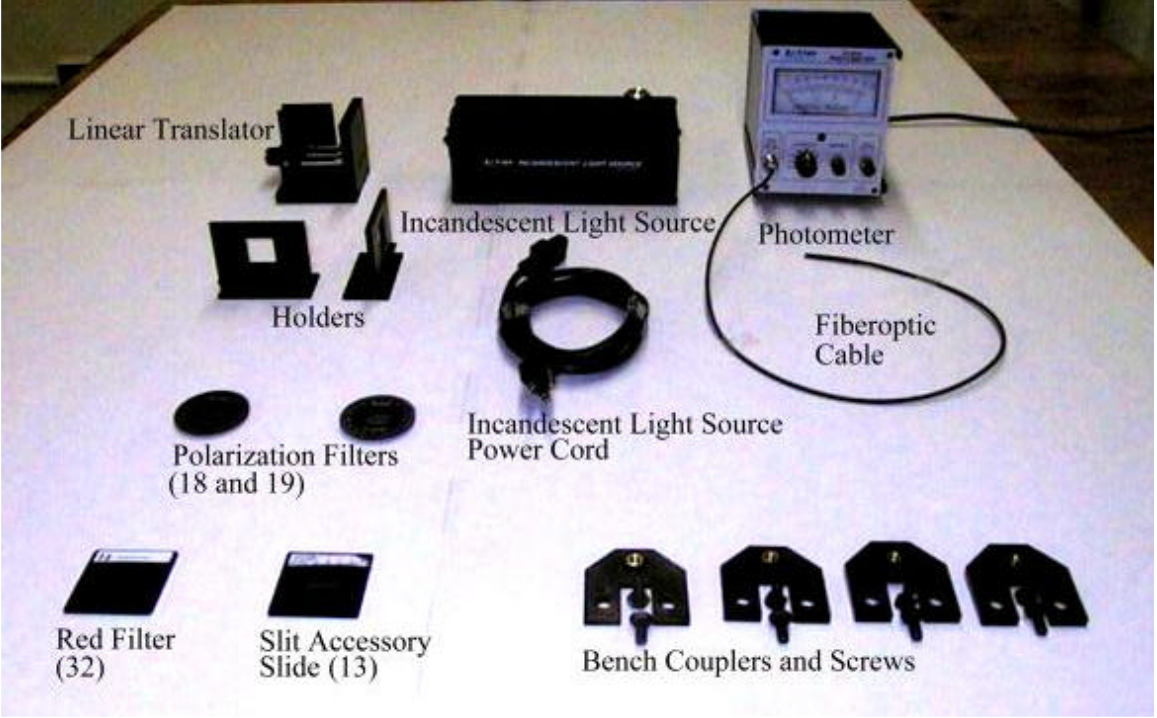
\includegraphics[width=0.8\textwidth]{./Exp7/pic/image8.png}
\caption{Equipment Components}
\label{fig:setup}
\end{figure} 

\section{Equipment}
\indent\indent\underline{Linear Translator:}
A holder for the fiberoptic cable that can be moved transversely in small increments, allowing a positioning with better than $0.1\,\mathrm{mm}$ precision. \myskip

\underline{Fiberoptic Cable:}
Cable made from glass, quartz, plastic or a similar material, which carries light waves. The cable uses total internal reflection at the walls to provide very high efficiency (or low losses) between the cable ends.\myskip

\underline{Photometer:}
Device to measure the total power contained in light impinging on it. It uses the photoelectric effect to convert the photons to electrons and various electron amplification techniques to produce a measurable electric current.

\subsection{Polarization}
\begin{itemize}
\item Make sure only the dim incandescent ceiling lights in the room are on.

\item The linear translator should be placed at the far end of the track opposite the laser. Make sure that the linear translator is in the middle position (at $2.5\,\mathrm{cm}$).

\item Place the fiber-optic cable in the hole of the linear translator.

\item Place the incandescent light source about $10$-$20\,\mathrm{cm}$ from the linear translator such that the light shines towards the linear translator.

\item Place the polarizers (numbers 18 and 19) in the holders.

\item Rotate the polarizers such that the white mark on the holder aligns with the $0^{\circ}$ angle reading on the polarizer.

\item Place the two polarizers between the incandescent light source and the linear translator.

\item Put the photometer to the lowest sensitivity (the 1000 setting) and use the zero adjust knob to make sure that the pointer is at the 0 position when the incandescent light source is turned off. 

\item Turn the incandescent light source back on and adjust the sensitivity of the photometer such that the needle is at the highest position without being at the maximum reading. The value of the sensitivity corresponds to the maximum value on the analog scale.

\item Record this measurement as the intensity for $0^{\circ}$ difference between the two polarizing axes.

\item Measure the intensity for angles between $0^{\circ}$ and $90^{\circ}$ in increments of 10 degrees. If the readings become too small you may have to switch the photometer to a setting with a higher sensitivity.

\item Plot the relative intensity ($I$ divided by $I_0$, the intensity at $0^{\circ}$) vs. the $\cos^2$ of the angle between the axes of the polarizers.

\item What is the general shape of your graph? What does this indicate? Did your line or curve pass through the origin?

\item What reading do you obtain when the polarizers are at an angle of $90^{\circ}$ relative to each other? (This is called the ``noise'' of your measuring device.) What reading would you expect if there was no noise?

\item What is the signal to noise ratio? (The ``signal'' is the reading at $0^{\circ}$.) What does this tell you?

\item If you had a lot of background light, how could you reduce the influence it would have on your results (by changing the setting or by changing your data analysis)?

\item If you had aligned the $90^{\circ}$ mark instead of the $0^{\circ}$ mark of both polarizers with the white mark on the holder would your results have been any different? What relative intensity would you expect if the angle between the two polarizers was $180^{\circ}$? $270^{\circ}$?

\item What are the main sources of error? Which do you think contributes most?
\end{itemize}

\subsection{Double Slit}
\begin{itemize}
\item Before you start this section, be sure you have read the laser safety note above.

\item Your TA will demonstrate the interference pattern by projecting it on the wall. Note down your observations!

\item Remove the incandescent light source, the polarizors, and the holders from the track, and the fiberoptic cable from the linear translator.

\item The laser should already be mounted on the laser holder at the far end of the track. Rotate the dial on the linear translator so that it is in the middle position.

\item Turn on the laser. It should propagate through the center of the hole in the linear translator, producing a bright red dot on the wall. If the laser is not properly aligned, alter the position of the laser by adjusting \emph{only the back legs} on the laser holder. Make sure you avoid lifting the laser and shining it in your classmates' eyes.

\item Place the red filter (number 32) onto the linear translator. Carefully slide the fiberoptic cable back into the hole in the linear translator so that the front of the cable sits right against the red filter.

\item Place the slide with the slits (number 13) in a holder and place the holder right in front of the laser.

\item Adjust the slide position in the holder so that the laser propagates through slit pattern A.

\item Note the interference pattern on the front of the linear translator.

\item Adjust the photomoter sensitivity to an appropriate setting.

\item Turn the knob on the linear translator. This should cause the intensity reading on the photometer to change.

\item Record the position and intensity for each maximum until the linear translator has moved as far as possible, starting from the 0 position of the linear translator. As you turn the knob on the linear translator take care not to shift the position of the linear translator on the bench.

\item Measure and record the distance $L$ from the slits to the tip of the fiberoptic cable. Where is the $0^{\mathrm{th}}$ order maximum located? Why might it be located somewhere other than the middle position of the linear translator?

\item Plot the position of the maxima $x_{m}$ vs. the order $m$. Determine the slope of your graph and use it to calculate the wavelength of the laser light. The slit separation for slit A is $0.250\, \mathrm{mm}$.

\item Construct a graph of the relative intensity, $I/I_{0}$, vs. $x_{m}$. Explain the shape of your graph.

\item Would the maxima be more spread out or closer together if the slit separation decreased?

\item Remove the slit slide and its holder from the track and the fiberoptic cable from the linear translator. Rotate the dial on the linear translator so that it is in the middle position.

\item Place the unknown slit apparatus on the track approximately $25\,\mathrm{cm}$ from the front of the laser so that the laser propagates through the slit pattern marked with a pink dot. You should see a horizontal interference pattern on the linear translator; the light in the center of the interference pattern should propagate through the hole in the linear translator. Note: If the laser does not propagate through the appropriate slit, slide the unknown slit apparatus towards and away from the laser until the laser strikes the slit pattern at the appropriate place. If the light from the pattern does not propagate through the center of the linear translator, alter the position of the laser by adjusting \emph{only the back legs} on the laser holder.

\item Again measure the distance between consecutive maxima as above. Also, measure the distance $L$ from the slits to the tip of the fiberoptic cable. Use this data and the wavelength of the laser you determined previously to determine the slit separation.

\item What is the purpose of using the red filter?

\item Give the main sources of error.
\end{itemize}

\section{Applications}
Some chemical molecules have a property called chirality. This means that the mirror image of the molecule is not identical to the original. For example, no matter how good you might be at 3D puzzles, you cannot arrange images of the molecule and of its mirror image to superimpose precisely. A famous example is the DNA double helix, a highly complex molecule, which carries all genetic information. The molecule always twists in one direction, while its mirror image always twists in the opposite direction. Many such chiral molecules are optically active, and rotate the polarization-axis of transmitted or reflected polarized light\footnote{For instance, the glucose dextrose turns the polarization axis to the right: ``dexeter'' is Latin for ``right''.}. If you shine polarized light into such a sample, you will see that the light leaving the sample has its polarization axis rotated a few degrees clockwise or counterclockwise, depending on the substance.\myskip

This effect can be used to determine the concentration of chiral molecules in a solution. For example, you can determine the glucose concentration in a blood specimen in a non-chemical way. The calculation of the concentration is particularly simple, since the change in angle of the polarization axis depends only on the concentration of the chiral substance in the solution, the distance the light travels through the sample, and a constant specific for the substance. Calculating the glucose concentration, therefore, requires only a measurement of the rotation in polarization vector and known constants -- a simple task for a rudimentary computer. 

\newpage
\section{Lab Preparation Examples}
\underline{Polarization:}
\begin{enumerate}
\item You look at the sky through a polarizer and as you turn the polarizer you see that the sky appears darker or lighter, depending on the position of the polarizer. What does this observation tell you?

\item You look at a light source through a polarizer. As you turn the polarizer you see no change in intensity. Is the light emitted by this source polarized?

\item Unpolarized light passes through two polarizers whose polarization axes are aligned. You note down the observed intensity as $I_{0}$. Now you turn the polarization axis of one of the polarizers by $60^{\circ}$. What intensity do you observe now?

\item Now you add, after the second polarizer, a third polarizer. The third has a polarization axis of $30^{\circ}$ relative to the second polarizer. What intensity do you observe now?

\item Does the result depend on which of the two polarizers you rotate in question 3?

\item Would your answer to question 5 change if the light source produced polarized light? Explain!

\item You have two polarizers with an angle of $90^{\circ}$ between their polarization axes. Adding a third polarizer between these two polarizers will typically produce light after the final polarizer. At what angle (relative to the first polarizer's axis) would you observe the maximum intensity after the third polarizer?
\end{enumerate}

\underline{The Double-Slit:}

While performing a double slit experiment, with $L = 1.00\pm 0.01\,\mathrm{m}$, $d = 0.5\pm 0.1\, \mathrm{mm}$, you obtain the following locations for maxima:
\begin{table}[h]
  \centering
  \begin{tabular}{|c|c|c|c|c|c|c|c|c|c|}
    \hline
    order&-4&-3&-2&-1&0&1&2&3&4\\
    \hline
    Position (mm)&-4.1&-3.2&-2.0&-0.9&0.0&1.3&2.1&3.2&3.9\\
    \hline
  \end{tabular}
\end{table}
\begin{enumerate}\setcounter{enumi}{7}
\item Calculate x for all of the consecutive maxima and use the 2/3 estimate to determine the uncertainty of x. Now determine the wavelength of the light (including uncertainty).
\item Using the data above, determine x from a plot of position vs. order. Given the wavelength as $\lambda = 600\,\mathrm{nm}$ and $L = 1.00\pm 0.01\,\mathrm{m}$, what is the spacing between the two slits?
\end{enumerate}

\section{Appendix for Experts: How a Laser works (Not required!)}
Quantum mechanics tells us that light is produced when electrons in an atom make a transition from a higher to a lower state, or energy level. Whenever an electron makes a
transition between states, the difference in energy is emitted (or absorbed) as a discrete energy package called a photon\footnote{See the experiment on the Photoelectric Effect.}, which carries (with other photons) the electromagnetic wave. The transition from a higher to a lower state can happen in two different ways. First, it can happen randomly, i.e. the electron just falls down spontaneously. This is what happens when a candle produces light. Electrons that make such random transitions result in emitted photons which are incoherent, or out of phase with one another. \myskip
\begin{figure}[h]
\centering
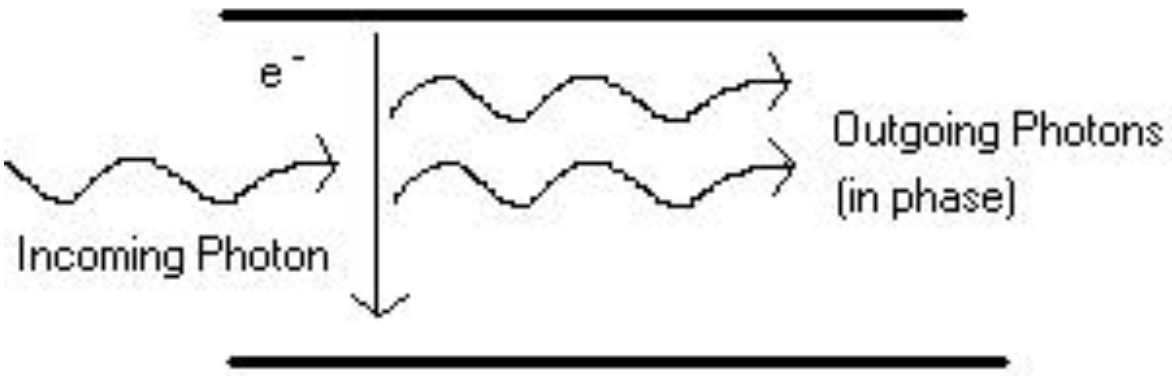
\includegraphics[width=0.5\textwidth]{./Exp7/pic/image9.png}
\caption{Process of Stimulated Emission}
\label{fig:stimulatedemission}
\end{figure} 

The second way this process can happen is called stimulated emission. If you already have a field of photons that are in phase and have the same frequency, and that frequency corresponds exactly to the transition energy, the emission is no longer random. When an electron falls to the lower energy level, a photon is emitted precisely in phase with the already existing photons, as shown in Figure {\ref{fig:stimulatedemission}}.\footnote{Photons are of a particle type called bosons. Such particles are highly ``social'' and like to be in exactly the same energy state and the same phase with their friends. This contrasts with another particle type, called fermions, which hate being in the same state as their associates (Pauli Exclusion Principle). Electrons are fermions, and this antisocial property accounts for the unique state of each electron in an atom. If electrons were bosons, all electrons in an atom would be in the ground state and we would not have chemistry!} In our analogy of soldiers marching on parade, new entrants to the parade are required to start walking in step with the others (or they would miss out on the parade).\myskip
\begin{figure}[h]
\centering
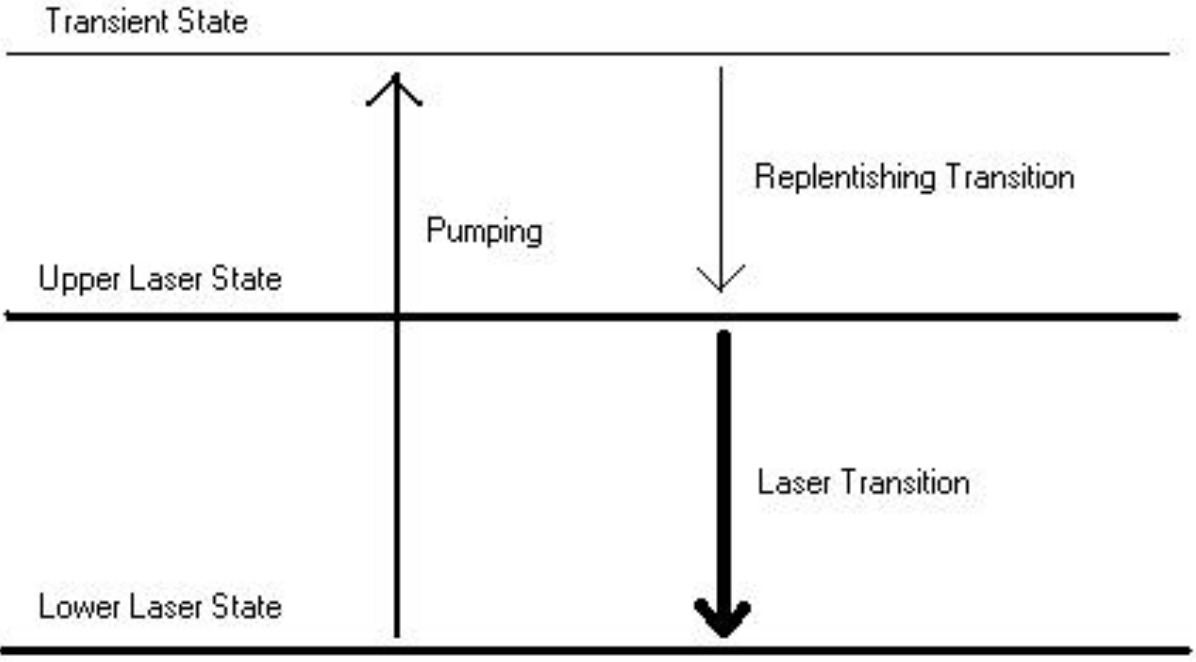
\includegraphics[width=0.5\textwidth]{./Exp7/pic/image10.png}
\caption{The basic three - level scheme for laser operation.}
\label{fig:transition}
\end{figure} 

For stimulated emission to work, the upper atomic state must be full of electrons and the lower one must be almost empty. This is called an inversion, since atoms (at ordinary temperatures) tend to be in their lowest energy state. The inversion is actually achieved by pumping the electrons from the lower state into a third transient state, with an energy even higher than the second laser state, so that the electrons fall down to replenish the upper laser state. So real lasers use at least three energy levels; efficient lasers usually use even more\footnote{Semiconductor lasers (or laser diodes) work somewhat differently, but the underlying concepts of stimulated emission and inversion are the same.}.\myskip

Finally, the setup is placed in a cavity with a mirror at one end and a semi-transparent\footnote{These semi-transparent mirrors are still highly reflective. They reflect about 99$\%$ of incident light to keep most of the light inside the cavity.} mirror at the other end. This increases the efficiency of the laser by maintaining a high density of laser light within the cavity. The little leakage emitted from the semitransparent mirror is actually what we use as the laser beam.

\chapter{Polarization and Interference}
\section{Introduction}
You have already investigated some wave properties last semester, so here we will expand upon your knowledge of waves and address three new concepts: polarization, interference and diffraction. Our experiment will be conducted with light waves, however the general concepts apply to many other waves as well.

\section{Theory}
\subsection{Polarization}
Polarization occurs only in transverse waves\footnote{Examples of transverse waves are oscillations on a string, water waves, or the electromagnetic radiation we treat here. Sometimes you may also hear the term polarization used in the context of transverse- and longitudinal polarization.}. By definition, the oscillation is perpendicular to the direction of wave propagation in a transverse wave. Since in three-dimensional space there are three independent dimensions, there are two possible perpendicular directions needed to describe any oscillatory motion perpendicular to the direction of motion. If you think about a transverse wave in a string, the oscillation could be up-and-down or left-and-right, while the wave front propagates forward along the string. The two independent and perpendicular directions are called the two polarization states. (Or in coordinates, if a wave propagates along the $z$-axis, there are two polarizations perpendicular to the wave motion--one along the $x$-axis and one along the $y$-axis.) Polarization cannot occur in longitudinal waves because the direction of oscillation has only one possibility, along the direction of motion.\myskip

You may argue that you can make oscillations happen on a string in more than just the two directions described above--and you are right! For example, you can make oscillations diagonally from the upper left to the lower right or you can even make circular oscillations by moving your hand continuously in a circle, producing a corkscrew pattern along the string\footnote{This wave is sometimes called left- or right- circular polarization.}. But no matter which wave you make, the oscillations can always be represented as two superimposed waves with displacements along the two mutually perpendicular polarization axes. Any vector can always be described by decomposing it into its $x$- and $y$- components. Here, the relevant vector is the oscillating displacement from the $z$-axis. The amplitudes of the resolved $x$ and $y$ components indicate how much of the wave is in each polarization state.\myskip

For electromagnetic radiation, the oscillating quantities are the electric (and magnetic) fields. These undulate perpendicular to the direction of the wave. Like waves in a string, electromagnetic waves are transverse waves and have polarization properties. The polarization state describes the axis along which the electric field in the wave oscillates. Visible light is electromagnetic radiation in a particular frequency-wavelength regime, with large frequency of oscillation ($\sim 10^{15}\,\mathrm{Hz}$) and small wavelength ($\sim 0.5\times 10^{-6}\, \mathrm{m}$).\myskip

\subsection{Polarizer}
Usually light is produced (e.g. incandescent light from a candle or a light bulb) by hot electrons and atoms, which are moving or are oriented in random directions, so that the wave is \textbf{unpolarized}. This means that the electric field associated with the wave oscillates in random directions (though always at right angles to the direction of the propagation of the light). So there is no favored direction for polarization. It is as if you were moving your hand in random directions at the end of a string. Note that this is very different from the cases of waves in a string described above. Even in circular polarization the oscillations were not random.
\begin{figure}[h]
\centering
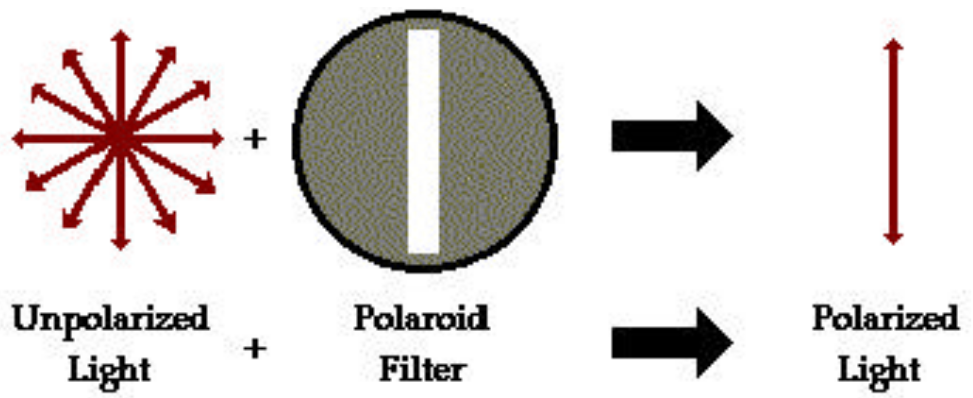
\includegraphics[width=0.5\textwidth]{./Exp7/pic/image1.png}
\caption{Polarization Filter and Creation of Polarized Light}
\label{fig:creation}
\end{figure}

A polarization filter, shown in Figure {\ref{fig:creation}}, is a device with a specified direction, called the polarization axis. The filter absorbs all the wave's incoming electric field perpendicular to the polarization axis and transmits the electric field parallel to the polarization axis. So no matter what the polarization of the light shining into a polarizer might be, the light coming out of the polarizer is always polarized in the direction specified by the polarization axis\footnote{Such light is called linearly polarized light.}. An unpolarized wave just prior to the polarizer has an electric field ($\mathbf{E}$) pointing randomly in all directions perpendicular to the wave direction, as shown in Figure {\ref{fig:detection}}. The polarized wave after the polarizer has only half the energy content, and the $\mathbf{E}$-field is oscillating solely along the polarization axis. This electric field has the same value as the component along that axis just before the polarizer.
\begin{figure}[h]
\centering
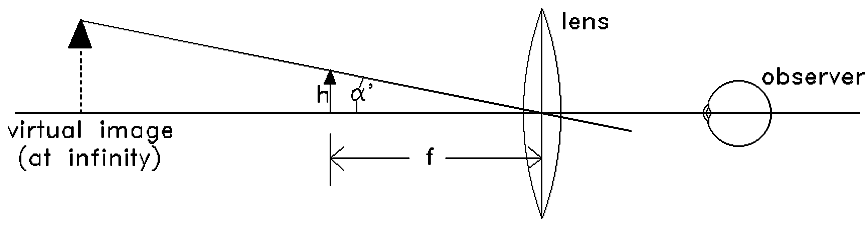
\includegraphics[width=0.8\textwidth]{./Exp7/pic/image2.png}
\caption{Detection of Polarized Light}
\label{fig:detection}
\end{figure}

\subsection{Interference--The Double Slit}
As you've learned in class, Young's double slit experiment is a demonstration of interference and diffraction. A double slit, as illustrated in Figure {\ref{fig:double}}, permits what remains of anincoming wave (from the left) to travel to a distant screen (to the right) along two different paths with different lengths. The light waves from the two slits interfere, resulting in an interference pattern of bright (constructive) and dim (destructive) patches as viewed on the screen. Let's see how the double slit works using Figure {\ref{fig:double}}.
\begin{figure}[h]
\centering
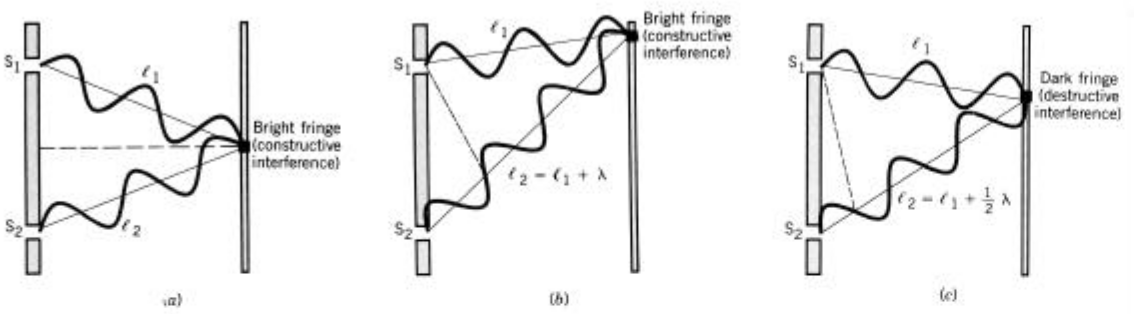
\includegraphics[width=0.8\textwidth]{./Exp7/pic/image3.png}
\caption{Young's Double Slit Experiment}
\label{fig:double}
\end{figure}

We shine light from the left onto the double slit, which allows two light waves to propagate from the two slits. Straight-ahead they will always be in phase since they travel the same distance to the screen. But when the two waves propagate at an angle $\theta$, they cover different distances to reach a specific point on the screen. (We assume that the two rays are parallel, a good approximation since the screen is effectively infinitely far away compared to the distance between the two slits.)\myskip
\begin{figure}[h]
\centering
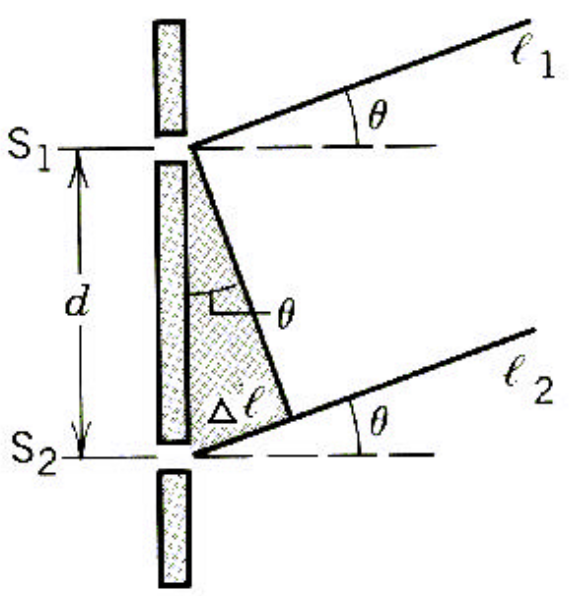
\includegraphics[width=0.3\textwidth]{./Exp7/pic/image4.png}
\caption{Geometry of the Double Slit}
\label{fig:geometry}
\end{figure}

As you can convince yourself by applying the rules of trigonometry to the triangle in Figure {\ref{fig:geometry}}, the difference in path ($\Delta l$) between the two rays is, for slit separation, $d$,
\begin{equation}
  \Delta l =d\sin\theta
\end{equation}

So what quantitatively determines a point of maximum intensity on the screen? Maximum intensity occurs if the two waves are precisely in phase at that point on the screen. This follows from what you learned about constructive and destructive interference in the lab on standing waves. As you saw, two waves can add up constructively or destructively. In the case of maximal constructive interference, the waves combine at the screen so that a crest on one wave coincides with a crest on the other wave and a trough coincides with a trough. In the case of maximal destructive interference, the waves combine so that a crest on one wave coincides with a trough on the other wave. \myskip

The waves will be in phase when they meet at the screen if the path difference between the two waves is an exact number of wavelengths, $m$, where $m$ is an integer called the order of the maximum. This requirement, expressed mathematically, is
\begin{equation}
  \Delta l =m\lambda
\end{equation}

Note that if $m=0$, there is no difference in the path lengths, resulting in a maximum straight ahead, $\theta=0$, as shown in Figure {\ref{fig:interference}}. Subsequent maxima occur for subsequent positive and negative integers, $m=\pm 1, \pm 2, \pm 3, \dots$. \myskip

Combining the two equations for $\Delta l$, we get for the specific angles, $\theta_{m}$ , that give maximal constructive interference:
\begin{equation}
  d\sin \theta_{m}=m\lambda
\end{equation}

If we know the order $m$ of a particular maximum, we can determine the wavelength of the light incident on the double slit by measuring the angle of the maximum on the screen. Conversely, we can determine the order of a particular maximum, $m$, from the wavelength of the light and the angle.
\begin{figure}[h]
\centering
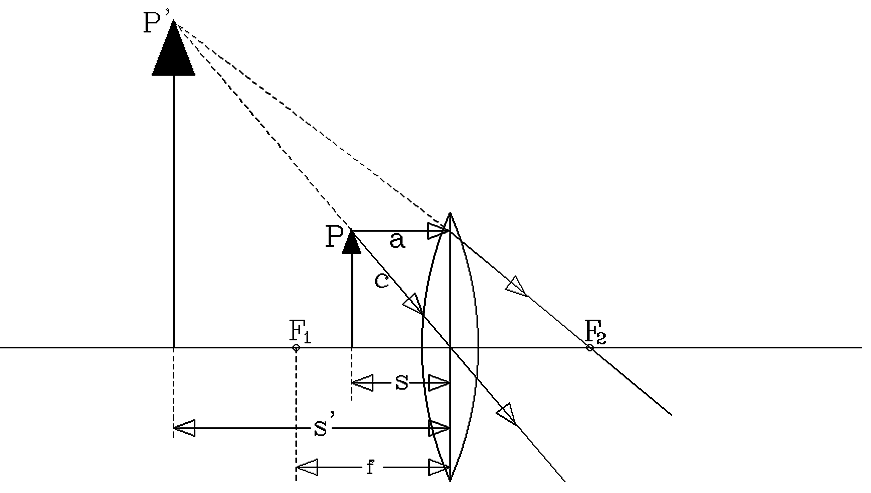
\includegraphics[width=0.6\textwidth]{./Exp7/pic/image5.png}
\caption{Interference of Light Coming from Two Small Slits}
\label{fig:interference}
\end{figure}

\subsection{Intensity of the Double-Slit Maxima}
You will soon note that the intensities for subsequent maxima are different. What causes this? Just as the double slit creates an interference pattern, each single slit creates a diffraction pattern due to interference from waves coming from different parts of a single slit as described in section 39-6 of the lecture course text\footnote{Sears, Zemansky, and Young, \textbf{College Physics \engordnumber{7} edition}, Addison-Wesley, p. 903-906.}. This occurs because each individual slit has a finite width. The overall (more realistic) pattern shown in figure {\ref{fig:intensity}} is a superposition of the single slit and double slit interference patterns. The narrow spikes (of interest for this experiment) are due to the double slit interference and the envelope, or large-scale pattern, is due to the single slit diffraction caused by each slit.
\begin{figure}[h]
\centering
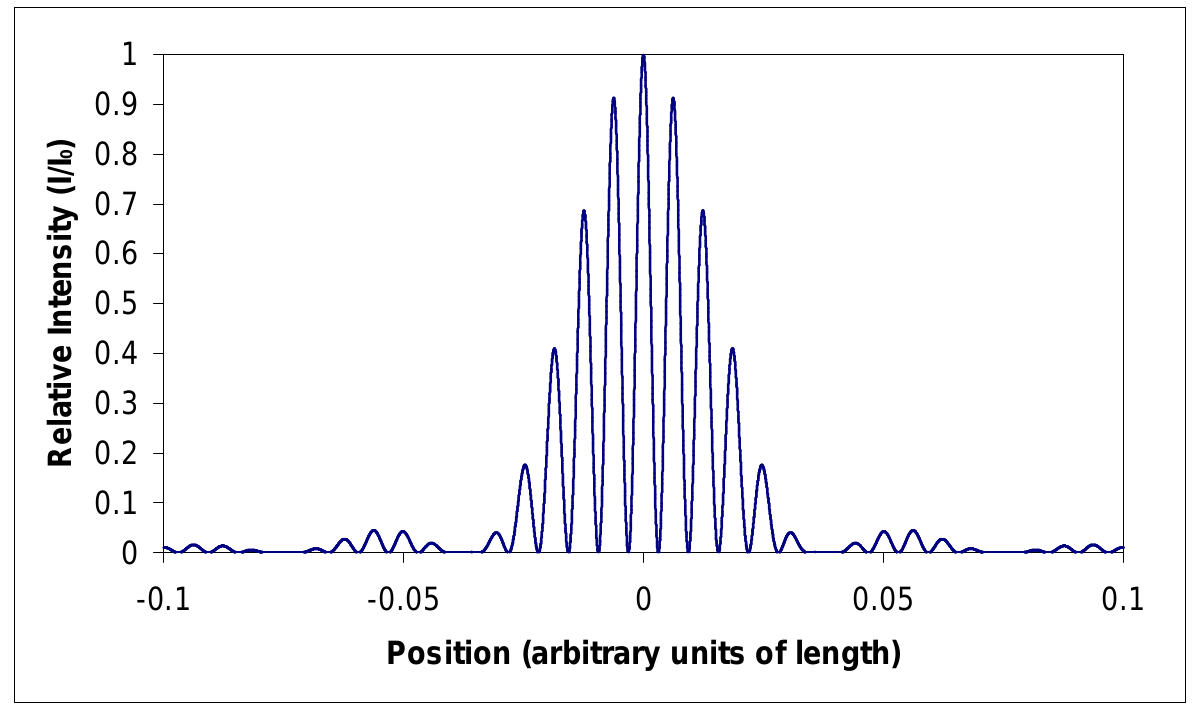
\includegraphics[width=0.8\textwidth]{./Exp7/pic/image6.png}
\caption{Intensity Pattern of the Double Slit. The Many Peaks of the Narrow Spikes Correspond to the Maxima in $d\sin\theta_{m}=m\lambda$}
\label{fig:intensity}
\end{figure}

\subsection{Light from a Laser}
In the double slit experiment we use a laser as the light source. Laser light differs from incandescent or fluorescent light in two important ways. First, lasers emit intense light of a single wavelength or frequency (monochromatic). Second, laser light is coherent, meaning that all light waves are in phase.\myskip

 Let's illustrate the differences between coherent and incoherent light through a simple familiar example. Contrast a crowd of people cramming the city streets during rush hour with a regiment of soldiers at a parade. In the midtown crowd, even if everybody were to step at the same frequency (which they don't!), each pedestrian's steps are independent of what others are doing. But soldiers at a parade move in step, or in phase, with a similar frequency, taking their steps at exactly the same time. Laser light is like the (coherent) soldiers at a parade, whereas light from a light bulb is like the (incoherent) civilian crowd at Times Square.\myskip

Although incandescent light sources\footnote{This is easily visible in the colors produced by soap bubbles.} can produce diffraction and interference patterns, a laser is better suited to illustrate coherent phenomena.

\section{Experiments}
\subsection{Polarization}
Suppose a wave has linearly polarized light characterized by an electric field vector, $\mathbf{E}_{0}$, at an angle, $\phi$ , relative to the direction of a polarizer. The electric field that is transmitted through the polarizer is $\mathbf{E}=\mathbf{E}_{0}\cos\phi$, the component that was not absorbed. Since the energy intensity in the wave is proportional to $\mathbf{E}^2$, then the intensity passing through two polarizers will be proportional to the square of the cosine of the angle φ between the two polarizing axes.\footnote{This relation is sometimes referred to as Malus' Law, after Etienne Malus, who also discovered the polarization of reflected light in the early nineteenth century.}
\begin{equation}
  I=I_{\mathrm{max}}\cos^2\phi
\label{eq:i}
\end{equation}

In this experiment, we use an incandescent unpolarized light source and then polarize it by first passing it through a polarizer. The electric field vector $\mathbf{E}_{0}$ will then point along the same direction as the polarizing axis of the first polarizer. As the now polarized light falls on the second polarizer, only the component of $\mathbf{E}_{0}$ along the polarizing axis of the second polarizer will make it through unaffected. \myskip

As figure {\ref{fig:polarized}} illustrates, an electric field strength of only $\mathbf{E}_{0}\cos\phi$ will make it through the second polarizer, so that the new intensity will be given by Equation {\ref{eq:i}} above. A human eye or a photometer can detect this change in light intensity.
\begin{figure}[h]
\centering
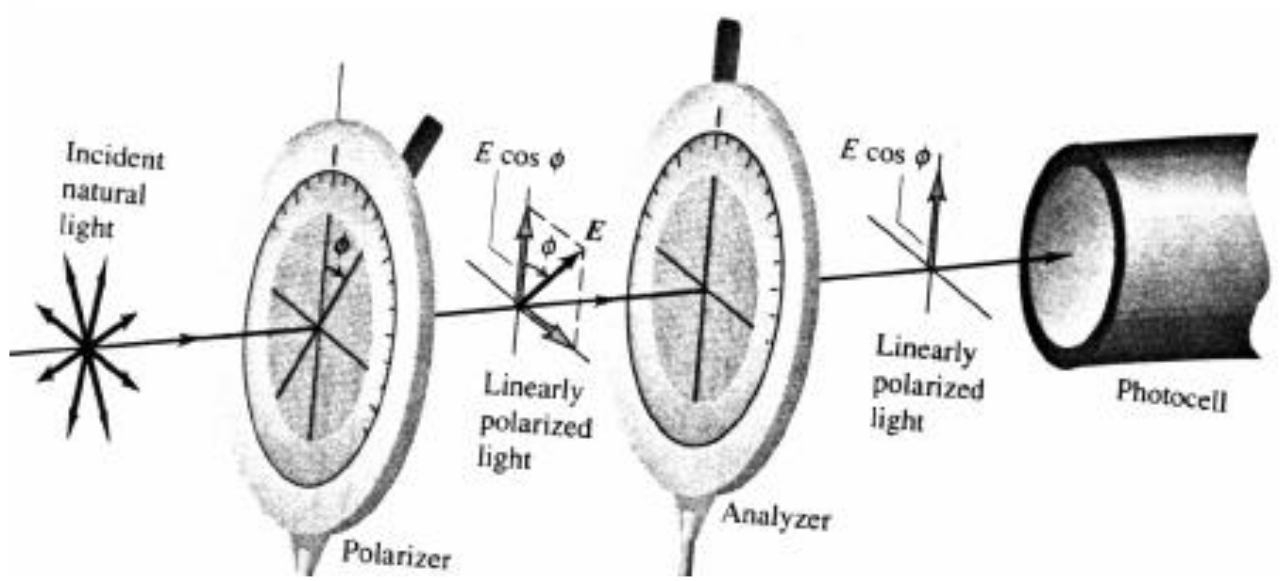
\includegraphics[width=0.8\textwidth]{./Exp7/pic/image7.png}
\caption{Creation and Detection of Polarized Light}
\label{fig:polarized}
\end{figure}

\subsection{Double Slit}
In this part of the experiment we use a laser instead of incandescent light source. Laser light shines onto a double slit, which produces an interference pattern of bright and dark lines on the wall or a piece of paper beyond the double slit. \myskip

We know that the angle, $\theta_{m}$, at which the $m^{\mathrm{th}}$ order bright spot appears is given by
\begin{equation}
  d\sin\theta_{m}=m\lambda
\end{equation}

For small $\theta_{m}$ (in radians), the approximation $\sin\theta \approx \tan\theta \approx \theta$ is valid\footnote{See for yourself by punching $\sin 0.1$ and $\tan 0.1$ into your calculator (using radiant measure)!}. So on a screen far away from the double slit, we observe maxima located close to the optical axis (where the $0^{\mathrm{th}}$ order maximum hits the screen) approximately given by
\begin{equation}
\sin\theta_{m}\approx\tan\theta_{m}=\frac{x_{m}}{L}
\end{equation}
where $x_m$ is the distance between the $m^{\mathrm{th}}$ order maximum and the $0^{\mathrm{th}}$ order maximum, and $L$ is the distance between the double slit and the screen. We then find
\begin{equation}
\frac{x_{m}}{L}=m\frac{\lambda}{d}
\end{equation}
or for adjacent maxima
\begin{equation}
  \frac{\Delta x}{L}=\frac{\lambda}{d}
\end{equation}
with $\Delta x$ equal to the distance between the maxima. Since $\Delta x$ and $L$ are easy to measure, we can straightforwardly determine $d$ (or $\lambda$ ) given $\lambda$ (or $d$).

\section{Specifics of the Experiment}
\underline{SAFETY NOTE:}

\emph{Although the laser is of low intensity for most situations, it can be dangerous in certain circumstances unless used carefully. In particular, \textbf{do not} use the laser in such a way that it can shine into any person's eye (The warning label on the laser states ``Do not stare into Beam!''). When you are not actually using the laser, turn it off or close the beam shutter at the front of the laser.}
\begin{figure}[h]
\centering
\includegraphics[width=0.8\textwidth]{./Exp7/pic/image8.png}
\caption{Equipment Components}
\label{fig:setup}
\end{figure}

\section{Equipment}
\indent\indent\underline{Linear Translator:}
A holder for the fiberoptic cable that can be moved transversely in small increments, allowing a positioning with better than $0.1\,\mathrm{mm}$ precision. \myskip

\underline{Fiberoptic Cable:}
Cable made from glass, quartz, plastic or a similar material, which carries light waves. The cable uses total internal reflection at the walls to provide very high efficiency (or low losses) between the cable ends.\myskip

\underline{Photometer:}
Device to measure the total power contained in light impinging on it. It uses the photoelectric effect to convert the photons to electrons and various electron amplification techniques to produce a measurable electric current.

\subsection{Polarization}
\begin{itemize}
\item Make sure only the dim incandescent ceiling lights in the room are on.

\item The linear translator should be placed at the far end of the track opposite the laser. Make sure that the linear translator is in the middle position (at $2.5\,\mathrm{cm}$).

\item Place the fiber-optic cable in the hole of the linear translator.

\item Place the incandescent light source about $10$-$20\,\mathrm{cm}$ from the linear translator such that the light shines towards the linear translator.

\item Place the polarizers (numbers 18 and 19) in the holders.

\item Rotate the polarizers such that the white mark on the holder aligns with the $0^{\circ}$ angle reading on the polarizer.

\item Place the two polarizers between the incandescent light source and the linear translator.

\item Put the photometer to the lowest sensitivity (the 1000 setting) and use the zero adjust knob to make sure that the pointer is at the 0 position when the incandescent light source is turned off.

\item Turn the incandescent light source back on and adjust the sensitivity of the photometer such that the needle is at the highest position without being at the maximum reading. The value of the sensitivity corresponds to the maximum value on the analog scale.

\item Record this measurement as the intensity for $0^{\circ}$ difference between the two polarizing axes.

\item Measure the intensity for angles between $0^{\circ}$ and $90^{\circ}$ in increments of 10 degrees. If the readings become too small you may have to switch the photometer to a setting with a higher sensitivity.

\item Plot the relative intensity ($I$ divided by $I_0$, the intensity at $0^{\circ}$) vs. the $\cos^2$ of the angle between the axes of the polarizers.

\item What is the general shape of your graph? What does this indicate? Did your line or curve pass through the origin?

\item What reading do you obtain when the polarizers are at an angle of $90^{\circ}$ relative to each other? (This is called the ``noise'' of your measuring device.) What reading would you expect if there was no noise?

\item What is the signal to noise ratio? (The ``signal'' is the reading at $0^{\circ}$.) What does this tell you?

\item If you had a lot of background light, how could you reduce the influence it would have on your results (by changing the setting or by changing your data analysis)?

\item If you had aligned the $90^{\circ}$ mark instead of the $0^{\circ}$ mark of both polarizers with the white mark on the holder would your results have been any different? What relative intensity would you expect if the angle between the two polarizers was $180^{\circ}$? $270^{\circ}$?

\item What are the main sources of error? Which do you think contributes most?
\end{itemize}

\subsection{Double Slit}
\begin{itemize}
\item Before you start this section, be sure you have read the laser safety note above.

\item Your TA will demonstrate the interference pattern by projecting it on the wall. Note down your observations!

\item Remove the incandescent light source, the polarizors, and the holders from the track, and the fiberoptic cable from the linear translator.

\item The laser should already be mounted on the laser holder at the far end of the track. Rotate the dial on the linear translator so that it is in the middle position.

\item Turn on the laser. It should propagate through the center of the hole in the linear translator, producing a bright red dot on the wall. If the laser is not properly aligned, alter the position of the laser by adjusting \emph{only the back legs} on the laser holder. Make sure you avoid lifting the laser and shining it in your classmates' eyes.

\item Place the red filter (number 32) onto the linear translator. Carefully slide the fiberoptic cable back into the hole in the linear translator so that the front of the cable sits right against the red filter.

\item Place the slide with the slits (number 13) in a holder and place the holder right in front of the laser.

\item Adjust the slide position in the holder so that the laser propagates through slit pattern A.

\item Note the interference pattern on the front of the linear translator.

\item Adjust the photomoter sensitivity to an appropriate setting.

\item Turn the knob on the linear translator. This should cause the intensity reading on the photometer to change.

\item Record the position and intensity for each maximum until the linear translator has moved as far as possible, starting from the 0 position of the linear translator. As you turn the knob on the linear translator take care not to shift the position of the linear translator on the bench.

\item Measure and record the distance $L$ from the slits to the tip of the fiberoptic cable. Where is the $0^{\mathrm{th}}$ order maximum located? Why might it be located somewhere other than the middle position of the linear translator?

\item Plot the position of the maxima $x_{m}$ vs. the order $m$. Determine the slope of your graph and use it to calculate the wavelength of the laser light. The slit separation for slit A is $0.250\, \mathrm{mm}$.

\item Construct a graph of the relative intensity, $I/I_{0}$, vs. $x_{m}$. Explain the shape of your graph.

\item Would the maxima be more spread out or closer together if the slit separation decreased?

\item Remove the slit slide and its holder from the track and the fiberoptic cable from the linear translator. Rotate the dial on the linear translator so that it is in the middle position.

\item Place the unknown slit apparatus on the track approximately $25\,\mathrm{cm}$ from the front of the laser so that the laser propagates through the slit pattern marked with a pink dot. You should see a horizontal interference pattern on the linear translator; the light in the center of the interference pattern should propagate through the hole in the linear translator. Note: If the laser does not propagate through the appropriate slit, slide the unknown slit apparatus towards and away from the laser until the laser strikes the slit pattern at the appropriate place. If the light from the pattern does not propagate through the center of the linear translator, alter the position of the laser by adjusting \emph{only the back legs} on the laser holder.

\item Again measure the distance between consecutive maxima as above. Also, measure the distance $L$ from the slits to the tip of the fiberoptic cable. Use this data and the wavelength of the laser you determined previously to determine the slit separation.

\item What is the purpose of using the red filter?

\item Give the main sources of error.
\end{itemize}

\section{Applications}
Some chemical molecules have a property called chirality. This means that the mirror image of the molecule is not identical to the original. For example, no matter how good you might be at 3D puzzles, you cannot arrange images of the molecule and of its mirror image to superimpose precisely. A famous example is the DNA double helix, a highly complex molecule, which carries all genetic information. The molecule always twists in one direction, while its mirror image always twists in the opposite direction. Many such chiral molecules are optically active, and rotate the polarization-axis of transmitted or reflected polarized light\footnote{For instance, the glucose dextrose turns the polarization axis to the right: ``dexeter'' is Latin for ``right''.}. If you shine polarized light into such a sample, you will see that the light leaving the sample has its polarization axis rotated a few degrees clockwise or counterclockwise, depending on the substance.\myskip

This effect can be used to determine the concentration of chiral molecules in a solution. For example, you can determine the glucose concentration in a blood specimen in a non-chemical way. The calculation of the concentration is particularly simple, since the change in angle of the polarization axis depends only on the concentration of the chiral substance in the solution, the distance the light travels through the sample, and a constant specific for the substance. Calculating the glucose concentration, therefore, requires only a measurement of the rotation in polarization vector and known constants -- a simple task for a rudimentary computer.

\newpage
\section{Lab Preparation Examples}
\underline{Polarization:}
\begin{enumerate}
\item You look at the sky through a polarizer and as you turn the polarizer you see that the sky appears darker or lighter, depending on the position of the polarizer. What does this observation tell you?

\item You look at a light source through a polarizer. As you turn the polarizer you see no change in intensity. Is the light emitted by this source polarized?

\item Unpolarized light passes through two polarizers whose polarization axes are aligned. You note down the observed intensity as $I_{0}$. Now you turn the polarization axis of one of the polarizers by $60^{\circ}$. What intensity do you observe now?

\item Now you add, after the second polarizer, a third polarizer. The third has a polarization axis of $30^{\circ}$ relative to the second polarizer. What intensity do you observe now?

\item Does the result depend on which of the two polarizers you rotate in question 3?

\item Would your answer to question 5 change if the light source produced polarized light? Explain!

\item You have two polarizers with an angle of $90^{\circ}$ between their polarization axes. Adding a third polarizer between these two polarizers will typically produce light after the final polarizer. At what angle (relative to the first polarizer's axis) would you observe the maximum intensity after the third polarizer?
\end{enumerate}

\underline{The Double-Slit:}

While performing a double slit experiment, with $L = 1.00\pm 0.01\,\mathrm{m}$, $d = 0.5\pm 0.1\, \mathrm{mm}$, you obtain the following locations for maxima:
\begin{table}[h]
  \centering
  \begin{tabular}{|c|c|c|c|c|c|c|c|c|c|}
    \hline
    order&-4&-3&-2&-1&0&1&2&3&4\\
    \hline
    Position (mm)&-4.1&-3.2&-2.0&-0.9&0.0&1.3&2.1&3.2&3.9\\
    \hline
  \end{tabular}
\end{table}
\begin{enumerate}\setcounter{enumi}{7}
\item Calculate x for all of the consecutive maxima and use the 2/3 estimate to determine the uncertainty of x. Now determine the wavelength of the light (including uncertainty).
\item Using the data above, determine x from a plot of position vs. order. Given the wavelength as $\lambda = 600\,\mathrm{nm}$ and $L = 1.00\pm 0.01\,\mathrm{m}$, what is the spacing between the two slits?
\end{enumerate}

\section{Appendix for Experts: How a Laser works (Not required!)}
Quantum mechanics tells us that light is produced when electrons in an atom make a transition from a higher to a lower state, or energy level. Whenever an electron makes a
transition between states, the difference in energy is emitted (or absorbed) as a discrete energy package called a photon\footnote{See the experiment on the Photoelectric Effect.}, which carries (with other photons) the electromagnetic wave. The transition from a higher to a lower state can happen in two different ways. First, it can happen randomly, i.e. the electron just falls down spontaneously. This is what happens when a candle produces light. Electrons that make such random transitions result in emitted photons which are incoherent, or out of phase with one another. \myskip
\begin{figure}[h]
\centering
\includegraphics[width=0.5\textwidth]{./Exp7/pic/image9.png}
\caption{Process of Stimulated Emission}
\label{fig:stimulatedemission}
\end{figure}

The second way this process can happen is called stimulated emission. If you already have a field of photons that are in phase and have the same frequency, and that frequency corresponds exactly to the transition energy, the emission is no longer random. When an electron falls to the lower energy level, a photon is emitted precisely in phase with the already existing photons, as shown in Figure {\ref{fig:stimulatedemission}}.\footnote{Photons are of a particle type called bosons. Such particles are highly ``social'' and like to be in exactly the same energy state and the same phase with their friends. This contrasts with another particle type, called fermions, which hate being in the same state as their associates (Pauli Exclusion Principle). Electrons are fermions, and this antisocial property accounts for the unique state of each electron in an atom. If electrons were bosons, all electrons in an atom would be in the ground state and we would not have chemistry!} In our analogy of soldiers marching on parade, new entrants to the parade are required to start walking in step with the others (or they would miss out on the parade).\myskip
\begin{figure}[h]
\centering
\includegraphics[width=0.5\textwidth]{./Exp7/pic/image10.png}
\caption{The basic three - level scheme for laser operation.}
\label{fig:transition}
\end{figure}

For stimulated emission to work, the upper atomic state must be full of electrons and the lower one must be almost empty. This is called an inversion, since atoms (at ordinary temperatures) tend to be in their lowest energy state. The inversion is actually achieved by pumping the electrons from the lower state into a third transient state, with an energy even higher than the second laser state, so that the electrons fall down to replenish the upper laser state. So real lasers use at least three energy levels; efficient lasers usually use even more\footnote{Semiconductor lasers (or laser diodes) work somewhat differently, but the underlying concepts of stimulated emission and inversion are the same.}.\myskip

Finally, the setup is placed in a cavity with a mirror at one end and a semi-transparent\footnote{These semi-transparent mirrors are still highly reflective. They reflect about 99$\%$ of incident light to keep most of the light inside the cavity.} mirror at the other end. This increases the efficiency of the laser by maintaining a high density of laser light within the cavity. The little leakage emitted from the semitransparent mirror is actually what we use as the laser beam.

\chapter{The Spectrum of the Hydrogen Atom}
\section{Introduction}
In this experiment we will observe the discrete light spectrum one observes from a gas discharge lamp. We will see that the spectrum consists of a collection of sharp, single colored lines. We will be able to measure the wavelength of the light emitted quite precisely, usually better than 1 part in a thousand. Therefore it is crucial to make all calculations to 5 significant figures.

\section{Theory}
\subsection{The Spectrum of the Hydrogen Atom}
According to the classical theory of electro magnetism, atoms should radiate continuously and the electrons should fall into the nuclei within a short timespan. Obviously this is not the case since we have stable atoms. Therefore the classical description seems to be wrong. \myskip

Niels Bohr suggested an alternative theory for atoms, suggesting that the electrons can only exist in certain energy states and can only jump between these discreet states discontinuously. This discontinuity explains why we see a collection of sharp lines in a gas discharge lamp, and not a continuous spectrum as in a usual light bulb. \myskip

Bohr was able to derive the following formula for the energy of the energy levels only using natural constants
\begin{equation}
  E_{n}=-\frac{2\pi^2 me^4k^{2}_{e}}{n^2h^2}=-\frac{me^4}{h^2}\bigg(\frac{1}{8\varepsilon^{2}_{0}}\bigg)\frac{1}{n^2}
\end{equation}
Therefore the energy one gets for a transition from an initial level $n_i$ to a final level $n_f$ is $\Delta E = E_{n_{i}} - E_{n_{f}}$.\myskip 

This energy is then set free in the form of light and one can relate it to the wavelength via
\begin{equation}
  \frac{1}{\lambda}=\frac{f}{c}=\frac{\Delta E}{hc}=\frac{E_{n_{i}}-E_{n_{f}}}{hc}=R\bigg(\frac{1}{n^2_{f}}-\frac{1}{n^2_{i}}\bigg)
\label{eq:lambda}
\end{equation}
where $R$ is called the Rydberg constant, which is given by
\begin{equation}
  R=\frac{2\pi^2me^4k^2_{e}}{h^3c}=1.0974\times 10^{7}\, \mathrm{m}^{-1}
\end{equation}

\subsection{Resolving a Light Spectrum with a Grating}
A grating is a collection of small parallel slits. In our case the slits are so fine that we cannot see them any more. A grating has the nice property that light of different wavelength gets diffracted in different directions. Therefore one can resolve a continuous light spectrum (containing light of various wavelengths) into its components. \myskip

How does a grating do this trick? To understand this it is sufficient if we look at only two slits with a distance $d$ between them. ($d$ is also called the lattice constant)\myskip

We look at two light rays coming from the two slits. If the two rays travel perpendicular to the two slits the two waves will always be in phase, since they travel the same distance. But if the two rays propagate at an angle $\theta$ to the normal the two rays will have to travel different distances to reach the eye. (we always assume that the two rays are parallel, which is a good approximation since the eye is almost infinitely far away compared to the distance between the two slits.)
\begin{figure}[h]
\centering
\includegraphics[width=0.3\textwidth]{./Exp9/pic/image1.png}
\caption{Geometry of the Double Slit}
\label{fig:slit}
\end{figure} 

As you may convince yourself by looking at the graph, the difference in path between the two rays is
\begin{equation}
  \Delta l =d\sin\theta
\end{equation}

As in the lab about standing waves we can have different possibilities how these two rays add up. They can add up to form a node or they can add up to form an anti node (or something in between). To form a node every mountain shall be made lower and every valley shall be made higher. Therefore each hill from one wave should meet a valley from the other ray and vice versa. To get an antinode and therefore a maximum in the total motion of the wave every hill should meet a hill and every valley should meet a valley.
\begin{figure}[h]
\centering
\includegraphics[width=0.8\textwidth]{./Exp9/pic/image2.png}
\caption{Young's Double Slit}
\end{figure} 

How do we now achieve maximum intensity (node)? We always get this if the two waves are in phase which means that there fits an exact number of wavelength $m$ in the difference between the two waves, i.e.
\begin{equation}
  \Delta l=m\lambda
\end{equation}
$m$ is also called the order. If we now put the two equations for $\Delta l$ together, we get
\begin{equation}
  d\sin\theta=m\lambda
  \label{eq:dsin}
\end{equation}
\begin{figure}[h]
\centering
\includegraphics[width=0.6\textwidth]{./Exp9/pic/image3.png}
\caption{Interference of Light Coming from Two Small Slits}
\end{figure} 

This tells us that given the order $m$ we can determine the wavelength of the light we see through the grating by reading off the angle. This also works the other way around. (We can also get m by count up the orders starting with 0 at an angle of 0 degrees, and then count how often a particular color repeats as you go to higher or lower angles.)

\subsection{How to read a Vernier Scale}
With a usual ruler you can read distances up to a mm resolution. But if you would like to have a measuring device to read with a $0.1\, \mathrm{mm}$ resolution you have a problem. In principle you can scratch such a fine scale in the ruler, but in practice you can easily imagine that due to the width of the marks themselves such a scale would be almost impossible to read. That is why we use a trick and introduce a Vernier scale.\myskip
A Vernier scale works in the following way:

\begin{enumerate}[a)]
\begin{figure}[h]
\centering
\includegraphics[width=0.5\textwidth]{./Exp9/pic/image4.png}
\end{figure} 
\item If the zero points of the vernier and main scales are aligned, the first vernier division is 1/10 of a main scale division short of a mark on the main scale; the \engordnumber{2} vernier division is 2/10 of a main scale division short of the next mark on the main scale, etc., and the \engordnumber{10} vernier mark coincides with a main scale mark.

\begin{figure}[h]
\centering
\includegraphics[width=0.5\textwidth]{./Exp9/pic/image5.png}
\end{figure} 
\item If the vernier scale is now moved to the right until the \engordnumber{4} vernier division is lined up with the nearest main scale division to its right, the distance the 0 point of the vernier scale has moved past the 0 point on the main scale is 4/10 of a main scale division. Thus the vernier scale gives the fraction of a main scale division that the zero point of the vernier has moved beyond any main scale mark.
\begin{figure}[h]
\centering
\includegraphics[width=0.5\textwidth]{./Exp9/pic/image6.png}
\end{figure} 

\item In this last example, the zero line of the vernier scale lies between $1.5\,\mathrm{cm}$ and $1.6\,\mathrm{cm}$ on the main scale. The fraction of a division from $1.5\,\mathrm{cm}$ to the zero line can be determined as follows: Line number 6 of the vernier scale coincides with a line on the main scale, so the zero line on the vernier has moved 6/10 of a main scale division away from the main scale line 1.5. Hence, the reading, to the nearest hundredth, is 1.56. The maximum uncertainty is now $\pm 0.01\,\mathrm{cm}$, corresponding to the smallest division on the vernier scale. The use of the vernier has reduced the maximum uncertainty of the caliper measurement from $\pm 0.1\,\mathrm{cm}$ (without the vernier) to $\pm 0.01\,\mathrm{cm}$.
\end{enumerate}

In this experiment we will not use a simple Vernier scale since we do not measure distances, but we will use an angular Vernier scale to measure sub-divisions of angles. If you look at the main scale you will see that the scale is divided in half-degree steps. (You have slightly longer marks for the full degrees and shorter marks for the half degrees.) For angles the next smaller unit is not 1/10 th of a degree but minutes, which is 1/60 th of a degree. But since we can already read the scale up to 1/2 degree we need not have a Vernier scale with 60 devisions but with 30 divisions.\myskip

So you first use the 0 mark on the Vernier scale to read off the angle in degrees and if you are in between 0 and 30 minutes or 30 and 60 minutes. Then you look which of the
markes on the Vernier scale exactly matches a mark on the other scale. So e.g. if the 0 mark on the Vernier scale is between 20.5 and 21 degrees and the \engordnumber{13} mark on the
Vernier scale matches a mark on the degree scale we would have a reading of $20 + 1/2+ 13/60$ degrees or 20 degrees and 43 minutes.

\section{Experiments}
\begin{figure}[h!]
\centering
\includegraphics[width=0.8\textwidth]{./Exp9/pic/image7.png}
\caption{Schematic of the Spectrometer}
\end{figure} 

\subsection{Adjusting the Spectrometer}
The first part of the experiment will basically include the procedure to set up the equipment. This should be done with as much care as possible. Only then we will be able to measure the wavelength on the limit of our apparatus. If you don't set up the spectrometer correctly you will get systematical errors, which screw up your data. 

\subsection{Obtaining the Lattice Constant}
 After adjusting the spectrometer we will measure the yellow line of a Helium discharge lamp. Since we know that the wavelength of this light is $\lambda = 5.8756\times 10^{-7}\,\mathrm{m}$, we can determine the lattice constant of the grating quite accurately. Even though the lattice has written on it 600 lines/mm (which is only an approximate value anyway), we want to get the lattice constant with 5 relevant digits and not just 3, and this means that we have to measure it!

\subsection{Measuring the Spectrum of Hydrogen Atoms}
With the lattice constant determined in the previous part we now measure the wavelength of the light emitted from the Hydrogen discharge lamp. 

\section{Step by Step List}
\subsection{Adjusting the Spectrometer}
\begin{itemize}
\item Take the grating out off the holder and close the green knob.

\item Rotate the yellow knob such that the slit is about half open.

\item Look trough the eyepiece and turn the purple focusing ring until you see a sharp image of the slit.

\item Loosen the red knob and move the telescope tube until the cross hair is in the middle of the slit. Tighten red knob.

\item Now open the green knob and turn the tabletop such that the 0 mark from the Vernier scale with the magnifying glass is lined with either the 180 or the 360 from the outer scale. (Always use only this Vernier scale and don't switch to the other one in between)

\item Close the green knob (and don't open it again for the rest of the experiment!).

\item Now you can fine adjust the relative position of the inner and outer scale by turning the blue knob. Make sure that the lineup between the 0 on the Vernier and the 180/360 is done as careful as possible. (For some of the spectrometers there is a small mark to the left of the 0 mark on the Vernier scale. Make sure that you line up the 0 mark and not this extra mark with the 180/360.)

\item Now put the grating in the holder such that it is perpendicular to the telescope tube-collimator tube line. Close the white screw to lock the grating.
\end{itemize}

\subsection{Obtaining the Lattice Constant}
\begin{itemize}
\item Switch on the Helium lamp and line the spectrometer up such that you can see the slit well illuminated by the lamp as you look through the spectrometer.

\item Put the black cardboard over the front end of your collimator tube and you can use the black piece of cloth over the spectrometer to block light from the surrounding. Also this part and most important the next one should be performed in the dark, therefore switch off the light and use the lamps provided (they are supposed to be that dim) to read the scale.

\item Open the red knob and move the telescope tube to the left until the crosshair is in the center of the yellow line. (You should first see a few blue and green lines, then the isolated yellow line and then red lines. The yellow line should be somewhere around 20 degrees)

\item Note down the angle in degrees and minutes at which you see the \engordnumber{1} order of the yellow line. Do the same on the right side and average these two numbers.

\item Use the average and plug it into the grating equation ($m=1$) to determine the lattice constant $d$ (at least 5 relevant figures).

\item How many lines per mm does this lattice constant correspond to?

\item Can you also see the \engordnumber{2} order and \engordnumber{3} order yellow lines on either side?
\end{itemize}

\subsection{Measuring the Spectrum of Hydrogen Atoms}
\begin{itemize}
\item Now switch off the helium lamp and set up the spectrometer for the hydrogen lamp.

\item The light purple line you see in the middle is the $0^{\mathrm{th}}$ order and not yet one of the lines we are going to measure.

\item There are 4 visible lines for the Hydrogen spectrum. One red (furthest out), one greenish blue, one purple blue and one dark purple. The dark purple line is very
faint and you may not be able to see it, so don't despair.

\item Measure the angles of the 4 lines on both sides and average the angles.

\item How many orders do you see on either side? (look e.g. for the red line and count how often it appears as you go further out)

\item Do the higher orders overlap? (i.e. does a new order start before the old one ended?)
\end{itemize}

\subsection{Analyzing the Data}
\begin{itemize}
\item Put together formulas ({\ref{eq:lambda}}) and ({\ref{eq:dsin}}) and solve the resulting formula for $n_i$. 
\item Use your data and the value for $R$ from above and $n_f=2$ to determine $n_i$.
\item $n_i$ should be an integer number labeling from which initial atomic shell the electrons in the hydrogen atoms fell to the \engordnumber{2} atomic shell.
\item Are the results integers (or close to them)?
\item Are the numbers (integers) the one they are supposed to be?
\item For which color did the electrons jump from the lowest shell? Explain why you could have predicted that anyway!
\item Within how many \% have you been able to measure the data? Compare that to other experiments you have performed in this course!
\item Discuss briefly the factors that determine the uncertainty in your measurements. Which of them are random, which systematic?
\end{itemize}

\newpage
\section{Lab Preparation Examples}
\underline{Hydrogen Spectrum:}
\begin{enumerate}
\item What is the wavelength of emitted if an electron in an hydrogen atom makes a transition from $n_i=3$ to $n_f=1$?

\item For a hydrogen atom give all the transitions that fall within the visible range of the light spectrum (i.e. between $\lambda_{\mathrm{min}}=400\,\mathrm{nm}$ and $\lambda_{\mathrm{max}}=800\,\mathrm{nm}$). Give the transitions in the following form:
A transition from energy level $n_i=3$ to $n_f=1:3 \rightarrow 1$.\myskip

Hint: It may be simplest to calculate the energies $\lambda_{\mathrm{min}}=400\,\mathrm{nm}$ and $\lambda_{\mathrm{max}}=800\,\mathrm{nm}$ correspond to. Then make a list of $E_{n}$ and choose the differences between the energy
level that fit in the calculated range.

\item What wavelengths do the transitions in the previous problem correspond to?
\item If you look at the light of an object at high temperature (e.g. a normal light bulb), you will find that it usually emits a continuous spectrum without any gaps or lines in it. (This is due to the effect that the atoms in a solid (or plasma) are so close together that they disturb each other so strongly that the initially sharp transition lines of the atoms get so broadened that they appear as a continuous spectrum.)\myskip

But if you now look at the spectrum of the sun (or another star), you will find a continuous spectrum that has a number of sharp black lines, so no (or almost no) light of that frequency reaches you; the light of that frequency is missing in the spectrum. These black lines are at exactly the same positions where you would see the colored lines in emission spectra (that is what we do in lab) of the elements present on the sun. For example since hydrogen is present on the sun we will find black lines at the
wavelength calculated in 3.\myskip

Can you give a short explanation of how we get these inverse spectra (compared to the ones we see in the lab from emission spectra) from the sun? 
\end{enumerate}

\noindent\underline{Spectrum with a Grating:}
\begin{enumerate}\setcounter{enumi}{4}
\item What is the lattice constant $d$ if the lattice has 400 lines per mm?
\item If you have a grating with 600 lines per mm at what angle would you observe the $m=1$ maximum for a wavelength of $600\,\mathrm{nm}$?
\item If you have $d = 10^{-1}\, \mathrm{m}$ and $\lambda = 1\,\mathrm{cm}$. at what angles will you see the maxima for $m=1, 2, 3$?
\end{enumerate}

\chapter{Absorption of Beta and Gamma Rays}

\section{Introduction}

In this lab, we will study the behavior of gamma and beta rays as they pass through solid matter. Specifically, we will use beta ray absorption to measure the range of beta particles from a specific source and from that determine the energy of beta decay in Thallium 204. Additionally, we will determine the absorption coefficient of gamma radiation in lead from a Cesium 137 source.\myskip

The radioactive sources used in this experiment are all extremely weak and therefore can be handled without any danger of overexposure to radiation. However, it is always prudent not to handle any radioactive source more than is necessary.

\section{Theory}
\subsection{Nuclear Decay}
All nuclei heavier than lead (and many isotopes of lighter nuclei) have a non-zero probability of decaying spontaneously into another nucleus plus one or more lighter particles. One of the decay products may be an alpha-particle (two protons and two neutrons--the stable nucleus of a helium atom). Alternatively, a nucleus with more neutrons than it can maintain in stability may decay by emission of a beta-particle (a fast-moving electron or positron) which corresponds to the conversion of a neutron to a proton. These beta electrons may emerge with a kinetic energy of up to several MeV.\myskip

\begin{figure}[h]
\centering
\includegraphics[width=0.5\textwidth]{./Exp10/pic/image1.png}
\caption{Typical Nuclear Energy Level Diagram.}
\label{fig:level}
\end{figure}

After alpha or beta decay, the residual nucleus may be left in an excited state. In this case, a transition to a state of lower energy of the same nucleus will occur almost immediately with the emission of a photon (also called a gamma ray). The spectrum of photons emitted from the various excited states of a nucleus will have discrete frequencies $f$, corresponding to transitions $\Delta E=hf$, between discrete energy levels of the nucleus. The spectrum from an excited nucleus is thus \textbf{analogous} to the line spectrum of visible radiation from an atom due to excited electrons, with the notable difference that the MeV energy changes of the nucleus are approximately $10^6$ times as large as energy changes in transitions between atomic states (where $\Delta E_{\mathrm{atomic}}\approx$ several eV). See Figure {\ref{fig:level}}.\myskip

\begin{figure}[h]
\centering
\includegraphics[width=0.5\textwidth]{./Exp10/pic/image2.png}
\caption{Beta Ray (Electron) Energy Spectrum}
\label{fig:betaray}
\end{figure}

In early experiments on beta-decay, it was observed that each decay was not a simple one in which an electron and the recoil nucleus came off with equal and opposite momentum. The electrons, in fact, were emitted with a continuous spectrum of energies (as in Figure {\ref{fig:betaray}}). It was subsequently suggested by Pauli and Fermi that in each decay, another particle of zero mass and charge, called the neutrino, was emitted. Experimental verification of the neutrino has been obtained by observation of its rare interaction with matter.

\subsection{Detection of Charged Particles (the Geiger Counter)}
When an energetic charged particle traverses matter, it will give electrostatic impulses to nearby electrons and thus ionize atoms of the material. Most methods for detecting nuclear particles rely on observing the results of this ionization. For example, in a photographic emulsion, a trail of ionized grains will show up when the film is developed; in a cloud or bubble chamber, a trail of droplets or bubbles forms along the wake of ionization left by a charged particle; and in a scintillation counter, ionized molecules will very rapidly radiate visible light. In the \textbf{Geiger counter}, which will be used as a detector in this experiment, the ionization produced by a charged particle causes a violent electrical discharge.
\begin{figure}[h]
\centering
\includegraphics[width=0.5\textwidth]{./Exp10/pic/image3.png}
\caption{The Geiger Counter.}
\label{fig:counter}
\end{figure}

As shown in Figure {\ref{fig:counter}}, a Geiger counter comprises a metal cylinder (cathode) with insulating ends supporting a fine axial wire (anode). When a charged particle ionizes the gas (e.g., argon) in the tube, the resulting free electrons will move toward the positively charged anode wire, accelerated more and more by the rapid increase in electric field near the wire. When an electron acquires kinetic energy greater than the ionization energy of the gas molecules, it can create by collision a new ion and electron, which in turn can accelerate and create another ion, etc., thus initiating an avalanche of charge. The process, called the \textbf{Townsend avalanche}, is possible only if the voltage maintained between anode and cathode is sufficiently high.\myskip

The basic counter circuit, shown in Figure {\ref{fig:geiger}}, supplies a positive high voltage of up to 900 volts to the center wire. When an avalanche occurs, current flows through resistor $R$, the counter side of $R$ drops in potential, and this negative pulse is fed through capacitor $C$ to a stage of amplification and then to a scaling device.\myskip
\begin{figure}[h]
\centering
\includegraphics[width=0.8\textwidth]{./Exp10/pic/image4.png}
\caption{Geiger Counter Circuit.}
\label{fig:geiger}
\end{figure}

For a large enough value of $R$, the voltage drop across R would be sufficient to stop the discharge after a count has been recorded. This method of quenching the discharge, however, has the disadvantage of creating a long time constant, $\tau = RC$, for reestablishing voltage across the counter, i.e., of creating a long ``dead time'' during which the passage of another particle cannot be detected. The quenching can be achieved for a lower value of $R$ by adding halogen vapor to the gas to help absorb ion pairs. Nevertheless, the resultant dead time is substantial and must be taken into account when the particle flux is high.

\subsection{Energy Loss and Range of Beta Particles}
An incident particle in matter will continually lose kinetic energy as it ionizes atoms in the material (Figure {\ref{fig:ionizing}}) until it eventually comes to rest. The distance a particle can travel through a material before losing all of its kinetic energy and stopping is called its \textbf{range}. \emph{For a particle of known charge and mass, there will be a unique range associated with each incident energy}. A formula can be theoretically deduced for the rate of energy loss--and hence the range--of a particle (of known mass, charge, and initial velocity) in a particular ``stopping'' material (of known electron density and ionization potential).
\begin{figure}[h]
\centering
\includegraphics[width=0.5\textwidth]{./Exp10/pic/image5.png}
\caption{Ionizing Action of Incident Electron.}
\label{fig:ionizing}
\end{figure}

In each interaction with atomic electrons, however, an incident electron may be scattered through small or relatively large angles, and as it traverses the material it may follow a rather tortuous, winding path (especially at low energies). Therefore, the actual path of the electron may be considerably longer than the observed distance that it penetrates into the material. For this reason, the incident electron range is not sharply determined, and the theoretical calculation is of limited usefulness for electrons of less than $1\, \mathrm{MeV}$ energy.\myskip

In this experiment, therefore, we will use an approximate empirical relationship between range and energy for low energy electrons:
\begin{equation}
  r=\frac{0.412\, \mathrm{g}/\mathrm{cm}^2}{\rho}E^{1.29}
\label{eq:re}
\end{equation}
where $r$ is in cm, $E$ is in MeV, and $\rho$ is the density of the stopping material in $\mathrm{g} / \mathrm{cm}^3$. Note that the density of Aluminum is $2.702\,\mathrm{g} /\mathrm{cm}^{3}$.\myskip

(This result is described in: L. Katz and A. S. Penfold, ``Range-Energy Relations for Electrons and the Determination of Beta-Ray End-Point Energies by Absorption,'' Revs.Modern Phys. \textbf{24}, 1 (1952).)

\subsection{Absorption of Gamma Rays}
Gamma rays, or high-energy photons, can interact with matter by three distinct processes:
\begin{enumerate}[1)]
\item Compton Scattering: This refers to a photon-electron collision in which the energy lost by the scattered photon is given to the recoil electron.
\item Photoelectric Effect: The photon is absorbed by the atom as a whole, releasing an electron with kinetic energy equal to $E_{\gamma} - E_{b}$ , where $E_{\gamma}$ is the photon energy and $E_{b}$ is the relatively small binding energy of the electron in the shell from which it is released.
\item Pair Production: If the photon has energy greater than $1.02\, \mathrm{MeV}$, it can create an electron-positron pair in the neighborhood of a nucleus. The radiative source used in this experiment does \textbf{not} emit photons with energy greater than $1\, \mathrm{MeV}$.
\end{enumerate}

The probability of each of the three processes taking place in a given thickness of material depends on the energy of the photon and the atomic structure of the material. The \emph{total} probability for interaction of photons in lead (i.e., the sum of the probabilities of the three processes) varies with photon energy as indicated in Figure {\ref{fig:linear}}. The coordinate plotted on the graph is $\mu$, the \textbf{total linear absorption coefficient} in units of $\mathrm{cm}^{-1}$. It is defined by the equation:
\begin{equation}
  \frac{d N}{d x}=\mu N
\end{equation}
where $N$ is the number of incident photons and $dN$ is the number removed from the beam (i.e., absorbed) in an absorber of thickness $dx$ (in cm). Note that $dN$ and $dx$ are the calculus equivalents of infinitesimally small values of $\Delta N$ and $\Delta x$, respectively. As in any process where the rate of decrease is proportional to the number present (such as the discharge of a capacitor), the solution of this differential equation is:
\begin{equation}
  N(x)=N_{0}e^{-\mu x}
\label{eq:nx}
\end{equation}
where $N(x)$ is the number of photons passing through $x\,\mathrm{cm}$ of absorber and $N_0=N(x)$ at $x = 0$ , and $e$ is the base of natural logarithms.
\begin{figure}[h]
\centering
\includegraphics[width=0.8\textwidth]{./Exp10/pic/image6.png}
\caption{Linear Absorption Coefficient μ for gamma rays in lead as a function of energy.}
\label{fig:linear}
\end{figure}

\section{Procedure}
\subsection{Adjustments and Measurement of Errors in Counting}
\subsubsection{High Voltage Variations}

Every Geiger tube that is in good working order has a plateau region in which its counting rate is relatively insensitive to changes in the high voltage supply. Follow these steps to find the optimal measurement voltage for your Geiger counter.
\begin{itemize}
  \item Place a source under the tube and increase the high voltage from its lowest value until the tube just begins to count.
  \item Take 30 second counts while raising the voltage in 50 volt steps.
  \item At some point, the curve of counting rate vs. voltage levels off. You will know you have hit the plateau if for a 100-volt increase, your count rate only goes up a very small amount (less than 10\%).
\end{itemize}
Do not raise the voltage further as this may damage the tube due to continuous breakdown. Set the high voltage to a value on this plateau for the remainder of the experiment. If this procedure is followed correctly, high voltage variations may be ignored as a source of error.

\subsubsection{Statistical Accuracy}

Particles decay randomly in time from a radioactive source (over a period short compared to the half-life). The probability distribution for measuring a given number of these counts in a given time interval is an almost bell shaped curve (a Poisson Distribution) centered on $N_0$, the most probable value. The distribution will have a standard deviation about the peak of $\pm \sqrt{N_{0}}$ . If $N$ counts are measured in an interval, the best estimate of the error is $\pm \sqrt{N}$ .\myskip

Note that the magnitude of the statistical error--your uncertainty in the measurement--increases significantly for trials involving a very small number of counts. For a high counting rate in a given interval, say, 900 counts in one minute, the estimated error will be 30 counts per minute or 3.3\% error. However, for a much lower counting rate in the same interval, say 25 counts, the error of $\pm$5 counts per minute amounts to a 20\% statistical error. In order to achieve the same precision as in the first case, it would be necessary to collect 900 counts--in other words, to take a 36-minute measurement. While such a long measurement is impractical for this lab, you should keep in mind the relationship between a small number of counts and higher errors, and do your best to minimize these errors by taking longer measurements when necessary.

\subsubsection{Measuring Background Radiation}

In order to make accurate counting measurements of the sources, it is necessary to know the counting rate due to natural background radiation (mostly cosmic rays coming through the earth's atmosphere). Additionally, there will be some excess counts due to the Cs-137 gamma sources nearby in the room, whose gamma rays can pass through the side of the detector. At a distance of $30\,\mathrm{cm}$, for example, the Cs-137 source contributes roughly as many counts as the natural background radiation (doubling the distance would reduce its contribution to one-fourth this level). It's best to try to minimize these secondary effects -- by keeping your detector far from others' sources, and by shielding your own Cesium source with the lead sheets when not in use), but it's even more important to try to keep these background effects \emph{constant}. If all of your data is shifted by roughly the same constant amount, then it is possible to isolate the results you're interested in by subtracting out this constant background.

\subsection{Range of Beta Particles}
\begin{figure}[h]
\centering
\includegraphics[width=0.4\textwidth]{./Exp10/pic/image7.png}
\caption{Beta Absorption Curve}
\label{fig:beta}
\end{figure}
Thallium 204 beta decays to Lead 204 with a half-life of 3.9 years. The range of the most energetic of the decay electrons can be determined by placing aluminum foil absorbers between the source and the Geiger counter.\myskip

A typical absorption curve is shown in Figure {\ref{fig:beta}}. The maximum range $r$ is the point where the absorption curve meets the background. You should start by making a careful measurement of background, and you should repeat this measurement after taking the absorption curve to check for constancy.\myskip

Place the Thallium source on the second shelf below the detector, as shown in Figure {\ref{fig:absorption}}, to maximize the number of counts while leaving enough room to stack aluminum absorbers. Each of your measurements should be for a time interval of at least 30 seconds or until you get enough counts for a reasonable error.
\begin{itemize}
  \item Begin taking measurements and adding aluminum foil absorbers until the recorded count rate has lowered to the background level. Record the number of counts for each aluminum foil sheet added. (\emph{Note that the thickness of the aluminum absorbers is marked on the foil in \textbf{mils}, or thousandths of an inch, not millimeters}.)
  \item Take another measurement of the background to verify that everything has remained constant.
  \item Make a table of the results, including the background level, and include estimates of the statistical error in each measurement. Note that you \emph{should not} subtract background from your data for this experiment.
  \item With Microsoft Excel, make a plot of the log of your count rate vs. aluminum thickness. This is your beta absorption curve!
  \item Determine the approximate value of the maximum range $r$ from your graph and use Equation ({\ref{eq:re}}) to compare your result with the value of $E = 0.765\ \mathrm{MeV}$ for the maximum beta energy for Thallium 204 as measured in a magnetic spectrometer.
\end{itemize}

\begin{figure}[h]
\centering
\includegraphics[width=0.25\textwidth]{./Exp10/pic/image8.png}
\caption{Beta Absorption}
\label{fig:absorption}
\end{figure}

\subsection{Absorption of Gamma Rays}
The source for this part of the experiment is Cesium 137, which decays with a half-life of 30 years to Barium 137 with the emission of a $0.52\, \mathrm{MeV}$ beta ray (Figure {\ref{fig:cesium}}). The resulting Barium is in an excited state and decays by emitting a $0.662\, \mathrm{MeV}$ gamma ray almost instantaneously. Lead absorbers are used for the gamma absorption study. They are thick enough(0.062 inches) so that one absorber will stop all the betas.\myskip
\begin{figure}[h]
\centering
\includegraphics[width=0.5\textwidth]{./Exp10/pic/image9.png}
\caption{Cesium 137 Decay Scheme}
\label{fig:cesium}
\end{figure}

The gamma rays are detected by means of the same Geiger counter used in the previous part. Note that the efficiency of the Geiger counter for detecting photons is much less than for detecting the beta-particles, since it depends on a collision of the photon with the gas or wall of the counter, resulting in the emission of an electron, which in turn initiates the discharge.\myskip
\begin{figure}[h]
\centering
\includegraphics[width=0.5\textwidth]{./Exp10/pic/image10.png}
\caption{Scattering Effects: In (A), the gamma ray on the left passes outside of the detector tube. In (B), it can be seen how increasing the area of lead absorber can cause the same gamma ray to scatter \emph{into} the detector.}
\label{fig:scattering}
\end{figure}

Figure {\ref{fig:scattering}} represents one of the effects of gamma ray scattering in the lead sheets. Increasing the \emph{area} of lead through which the gamma rays pass tends to \emph{increase}, rather than decrease, the number of counts one measures, since gamma rays which otherwise would not have entered the detector may now be scattered into it.\myskip
\begin{figure}[h]
\centering
\includegraphics[width=0.4\textwidth]{./Exp10/pic/image11.png}
\caption{Absorption of Gamma Rays Set-Up.}
\label{fig:gammarays}
\end{figure}

The arrangement shown in Figure {\ref{fig:gammarays}} is designed to reduce the effect of such scattering. By keeping the lead sheets high above the source, one reduces the excess area exposed to gamma rays, and one reduces the effective difference in area between the top and bottom sheets as well.\myskip

\begin{enumerate}
  \item Take a measurement of the background count rate.
  \item Measure the number of counts per lead sheet thickness for as many sheets as you can fit in the apparatus. For your first measurement (for zero lead thickness) make sure the aluminum shelf is still present.\\ \\
  Note that gamma ray absorption differs fundamentally from beta absorption in the following way: there is no maximum range for gamma rays passing through lead; rather, one expects to lose a fixed fraction of the remaining gamma rays passing through each successive layer of lead absorber.

  \item Take another measurement of the background count rate to check for consistency. Use the average of these two count rates as your background for analysis.
  \item Make a table of data with error due to counting.
  \item With Microsoft Excel, make a plot of the log of count rate vs lead thickness with \emph{the  background count rate subtracted}. This exponential decay curve should appear as a straight line. Be sure to include error bars on your plot.
  \item Draw a line of best fit and determine error in the slope and intercept using LINEST.
  \item From Your slope, determine the absorption coefficient $\mu$ with error found by propagating uncertainties. Use your calculated value of $\mu$ and Figure \ref{fig:linear} to estimate the energy of the gamma rays.
  \item Does your calculated gamma ray energy agree with the accepted value (from Figure \ref{fig:cesium})?
  \item Discuss the main sources of error in determining gamma ray energy.
\end{enumerate}




\end{document}
